\documentclass[a4paper,adobefonts,11pt,UTF8]{book}

%type chinese characters
\usepackage{ctex}

%Bibliography
\usepackage{chapterbib}
\usepackage[sectionbib,square,super,sort&compress]{natbib}


%generate index of book
\usepackage{makeidx}

%modify the headheight at least 13.5pt
\usepackage[headheight=13.6pt]{geometry}

%
\usepackage{fontspec}

%unicode
\usepackage{xunicode}

%
\usepackage{xltxtra}

%mathematics package
\usepackage{amsmath}

%mathematics symbols
\usepackage{amssymb}

%origin print package
\usepackage{verbatim}

%draw graphics use tikz and so on.
\usepackage{graphicx}

%set graphics path which used in the book.
\graphicspath{{../img/}}

%colorful table
\usepackage{colortbl}

%set color use origin name directly.
\usepackage[svgnames,table]{xcolor}

%
\usepackage[figuresright]{rotating}

% generate longtable which could across pages.
\usepackage{longtable}

%
\usepackage{multirow}

%
\usepackage{adjustbox}


%
\newcommand\mgape[1]{\gape{$\vcenter{\hbox{#1}}$}}

%
\usepackage{array}

%
\usepackage{makecell}

%
\usepackage{ulem}

%
\usepackage{color}

% draw graphics use tikz package
\usepackage{tikz}

%
\usepackage{listings}
\lstset{
  basicstyle=\ttfamily,
  showstringspaces=false,
  commentstyle=\color{red},
  keywordstyle=\color{blue},
  columns=flexible,
  backgroundcolor=\color{lightgray},
  extendedchars=true,
  basicstyle=\footnotesize\ttfamily,
  showstringspaces=false,
  showspaces=false,
  numbers=left,
  numberstyle=\footnotesize,
  numbersep=9pt,
  tabsize=2,
  breaklines=true,
  showtabs=false,
  captionpos=b
}

%
\usepackage{bashful}

%set book information including bookmarksnumbered,pdfencoding,
%pdfauthor,pdfpagelayout,breaklinks,colorlinks,linkcolor,
%urlcolor,and so on.
\usepackage[bookmarksnumbered,pdfencoding=auto,pdfauthor={穷屌丝联盟},pdfpagelayout=TwoPageRight,breaklinks,colorlinks,linkcolor=RoyalBlue,urlcolor=blue,colorlinks=true]{hyperref}

%add more list types.
\usepackage{paralist}

%set page styles
\usepackage{fancyhdr}

\pagestyle{fancy}
\fancyhf{}
\fancyhead[LE,RO]{\thepage}
\fancyhead[RE]{\leftmark}
\fancyhead[RO]{\rightmark}
\fancypagestyle{plain}{
  \fancyhf{}
  \renewcommand{\headrulewidth}{0pt}
}


%titlepage \titleGM
\newcommand*{\plogo}{\fbox{$\mathcal{PL}$}} % Generic publisher logo
%--------------------------------------------------------------------
% TITLE PAGE
%--------------------------------------------------------------------

\newcommand*{\titleGM}{\begingroup % Create the command for including the title page in the document
\hbox{ % Horizontal box
\hspace*{0.2\textwidth} % Whitespace to the left of the title page
\rule{1pt}{\textheight} % Vertical line
\hspace*{0.05\textwidth} % Whitespace between the vertical line and title page text
\parbox[b]{0.75\textwidth}{ % Paragraph box which restricts text to less than the width of the page
{\noindent\Huge\bfseries Notes Collection of \\[0.5\baselineskip] PHP}\\[2\baselineskip] % Title
{\large \textit{PHP}}\\[4\baselineskip] % Tagline or further description
{\Large \textsc{theqiong.com}} % Author name

\vspace{0.5\textheight} % Whitespace between the title block and the publisher
{\noindent 穷屌丝联盟}\\[\baselineskip] % Publisher and logo
}}
\endgroup}
%


%lstlisting[language=JavsScript]
% Taken from Lena Herrmann at 
% http://lenaherrmann.net/2010/05/20/javascript-syntax-highlighting-in-the-latex-listings-package
\definecolor{lightgray}{rgb}{.9,.9,.9}
\definecolor{darkgray}{rgb}{.4,.4,.4}
\definecolor{purple}{rgb}{0.65,0.12,0.82}

%lstlisting package -----------
% JavaScript
%------------------------------
\lstdefinelanguage{JavaScript}
{
  keywords={typeof,new,ture,false,catch,function,return,null,switch,var,if,in,while,do,else,case,break},
  keywordstyle=\color{blue}\bfseries,
  ndkeywords={class,export,boolean,throw,implements,import,this},
  ndkeywordstyle=\color{darkgray}\bfseries,
  identifierstyle=\color{black},
  sensitive=false,
  comment=[l]{//},
  morecomments[s]{/*}{*/},
  commentstyle=\color{purple}\ttfamily,
  stringstyle=\color{red}\ttfamily,
  morestring=[b]',
  morestring=[b]"
}

\lstdefinelanguage{Scheme}
{morekeywords={,lambda, cond, case, display, let, import, quote, quasiquote, unquote,
define, begin, newline, if, list, apply, null?, car, cdr, or, not, and, for-each, 
make-vector, vector-length, vector-ref, vector-set!, eqv?, eq?, equal?, else, set!, 
define-record-type, fields, mutable, immutable, assert, parent, with-exception-handler, }
sensitive=false,
morecomment=[l]{;},
morecomment=[s]{/*}{*/},
morestring=[b]",
}

\lstdefinelanguage{CSS}{
  morekeywords={accelerator,azimuth,background,background-attachment,
    background-color,background-image,background-position,
    background-position-x,background-position-y,background-repeat,
    behavior,border,border-bottom,border-bottom-color,
    border-bottom-style,border-bottom-width,border-collapse,
    border-color,border-left,border-left-color,border-left-style,
    border-left-width,border-right,border-right-color,
    border-right-style,border-right-width,border-spacing,
    border-style,border-top,border-top-color,border-top-style,
    border-top-width,border-width,bottom,caption-side,clear,
    clip,color,content,counter-increment,counter-reset,cue,
    cue-after,cue-before,cursor,direction,display,elevation,
    empty-cells,filter,float,font,font-family,font-size,
    font-size-adjust,font-stretch,font-style,font-variant,
    font-weight,height,ime-mode,include-source,
    layer-background-color,layer-background-image,layout-flow,
    layout-grid,layout-grid-char,layout-grid-char-spacing,
    layout-grid-line,layout-grid-mode,layout-grid-type,left,
    letter-spacing,line-break,line-height,list-style,
    list-style-image,list-style-position,list-style-type,margin,
    margin-bottom,margin-left,margin-right,margin-top,
    marker-offset,marks,max-height,max-width,min-height,
    min-width,-moz-binding,-moz-border-radius,
    -moz-border-radius-topleft,-moz-border-radius-topright,
    -moz-border-radius-bottomright,-moz-border-radius-bottomleft,
    -moz-border-top-colors,-moz-border-right-colors,
    -moz-border-bottom-colors,-moz-border-left-colors,-moz-opacity,
    -moz-outline,-moz-outline-color,-moz-outline-style,
    -moz-outline-width,-moz-user-focus,-moz-user-input,
    -moz-user-modify,-moz-user-select,orphans,outline,
    outline-color,outline-style,outline-width,overflow,
    overflow-X,overflow-Y,padding,padding-bottom,padding-left,
    padding-right,padding-top,page,page-break-after,
    page-break-before,page-break-inside,pause,pause-after,
    pause-before,pitch,pitch-range,play-during,position,quotes,
    -replace,richness,right,ruby-align,ruby-overhang,
    ruby-position,-set-link-source,size,speak,speak-header,
    speak-numeral,speak-punctuation,speech-rate,stress,
    scrollbar-arrow-color,scrollbar-base-color,
    scrollbar-dark-shadow-color,scrollbar-face-color,
    scrollbar-highlight-color,scrollbar-shadow-color,
    scrollbar-3d-light-color,scrollbar-track-color,table-layout,
    text-align,text-align-last,text-decoration,text-indent,
    text-justify,text-overflow,text-shadow,text-transform,
    text-autospace,text-kashida-space,text-underline-position,top,
    unicode-bidi,-use-link-source,vertical-align,visibility,
    voice-family,volume,white-space,widows,width,word-break,
    word-spacing,word-wrap,writing-mode,z-index,zoom},
  morestring=[s]{:}{;},
  sensitive,
  morecomment=[s]{/*}{*/}
}








\setmainfont[Mapping=tex-text]{Minion Pro}

\makeindex


\title{{\zihao{1}PHP Notes}}
\author{{\zihao{3}穷屌丝联盟}}
\date{\today}








\begin{document}

\begin{titlepage}
\addcontentsline{toc}{part}{Cover}

\pagestyle{empty} % Removes page numbers

\titleGM % This command includes the title page


\end{titlepage}

\maketitle
\tableofcontents
\listoffigures
\listoftables
\printindex

\part{Introduction}

PHP\cite{php_wiki} is a server-side scripting language designed for web development but also used as a general-purpose programming language. PHP is now installed on more than 244 million websites and 2.1 million web servers. Originally created by Rasmus Lerdorf in 1995, the reference implementation of PHP is now produced by The PHP Group. While PHP originally stood for Personal Home Page, it now stands for PHP: Hypertext Preprocessor, a recursive acronym.

PHP\footnote{PHP:Hypertext Preprocessor,递归命名。}(Hypertext Preprocessor,超文本预处理器)是一种开源的通用计算机脚本语言,尤其适用于网络开发并可嵌入HTML中使用,现在大多数的Web主机都提供 PHP 的支持,而且使用PHP完全是免费的。

PHP code is interpreted by a web server with a PHP processor module, which generates the resulting web page: PHP commands can be embedded directly into an HTML source document rather than calling an external file to process data. It has also evolved to include a command-line interface capability and can be used in standalone graphical applications.

对于大多数的服务器,PHP 提供了一个模块,而且PHP 支持 CGI 标准,因而使得 PHP 能够作为 CGI 处理器来工作。作为一种免费的,并且使用广泛的创建动态交互性站点的强有力的服务器端脚本语言,对于像微软 ASP 这样的竞争者来说,PHP 无疑是另一种高效率的选项。

PHP is free software released under the PHP License, which is incompatible with the GNU General Public License (GPL) due to restrictions on the usage of the term PHP. PHP can be deployed on most web servers and also as a standalone shell on almost every operating system and platform, free of charge.



PHP最初由勒多夫在1995年开始开发,现在PHP的标准由PHP Group和开放源代码社区维护。PHP以PHP License作为许可协议,不过因为这个协议限制了PHP名称的使用,所以和开放源代码许可协议GPL不兼容。

PHP 文件的文件后缀是``.php"、``.php3" 或 ``.phtml",其中``.php"是 PHP 的默认扩展名,所有以 .php 结尾的文件都将由 PHP 来处理。在支持PHP的服务器上,只需要建立 .php 文件,并把它们放置到Web目录中,服务器将自动解析这些文件,不用编译任何东西,也不用安装任何其它的工具,仅仅只需把这些使用了 PHP 的文件想象成简单的 HTML 文件,其中只不过多了一种新的标识符,在这里可以做各种各样的事情。

PHP的主要目标是允许网络开发人员快速编写动态页面,其语法借鉴了C、Java和Perl等流行计算机语言的特点,易于一般程序员学习。使用 PHP 的一大好处是它对于初学者来说极其简单,同时也给专业的程序员提供了各种高级的特性,而且尽管 PHP 的开发是以服务端脚本为目的,但事实上其功能远不局限与此,PHP也被用于其他很多领域。


\zihao{6}



\begin{longtable}{|m{16pt}|m{20pt}|m{35pt}|m{300pt}|}

%head
\multicolumn{4}{r}{}
\tabularnewline\hline
主要\newline 版本	&次要\newline 版本	&发布日期	&说明
\endhead
%endhead

%firsthead
\caption{PHP版本历程}\\
\hline
主要\newline 版本	&次要\newline 版本	&发布日期	&说明
\endfirsthead
%endfirsthead

%foot
\multicolumn{4}{r}{}
\endfoot
%

%lastfoot
\endlastfoot
%endlastfoot

\hline
1.0		&1.0.0	&1995-06-08	&正式名称为``Personal Home Page Tools (PHP Tools)",第一次使用了``PHP"的名字。\\
\hline
2.0		&2.0.0	&1996-04-16	&针对PHP 1.0的改进版,速度更快、体积更小,更容易产生动态网页。\\
\hline
3.0		&3.0.0	&1998-06-06	&开发方式改成多人共同参与。Zeev Suraski和Andi Gutmans为了这个版本重写了剖析引擎。\\
\hline
\multirow{7}{40pt}{4.0}		&4.0.0	&2000-05-22	&改成以Zend引擎作为语法分析器,具有两阶段剖析/标签剖析系统等先进功能。\\ \cline{2-4}

		&4.1.0	&2001-12-10	&加入``超全局变量"(superglobals)功能,包含了\$\_GET、\$\_POST、\$\_SESSION等。\\  \cline{2-4}

		&4.2.0	&2002-04-22	&默认取消register\_globals功能。从网络接收的数据将不会设置成全局变量,增加程序安全性。\\ \cline{2-4}

		&4.3.0	&2002-12-27	&加入命令行可执行文件,称为CLI。\\ \cline{2-4}

		&4.4.0	&2005-07-11	&Added man pages for phpize and php-config scripts.\\ \cline{2-4}

		&4.4.8	&2008-01-03	&一些安全性的增强。曾可能为PHP 4的最后版本。若有必要,提供安全性更新到2008-08-08。\\ \cline{2-4}

		&4.4.9	&2008-08-07	&更多安全性增强和问题修补。PHP 4.4系列的最后版本。\\ \cline{2-4}
\hline
\multirow{18}{40pt}{5.0}		&5.0.0	&2004-07-13	&Zend Engine II with a new object model.\\ \cline{2-4}

		&5.1.0	&2005-11-24	&Performance improvements with introduction of compiler variables in re-engineered PHP Engine.\\ \cline{2-4}

		&5.2.0	&2006-11-02	&默认打开``过滤"的扩展。\\ \cline{2-4}

		&5.2.8	&2008-12-08	&emergent bug fix。\\ \cline{2-4}

		&5.2.9	&2009-02-26	&解决了5.2.*的超过了50多个错误和多个安全问题,增加了稳定性。\\ \cline{2-4}

		&5.2.10&2009-06-18	&这个版本修正了大量的bug和安全漏洞,并升级了时区数据库。\\ \cline{2-4}

		&5.2.17&2011-01-06	&修正了一个浮点数转化的Bug。\\ \cline{2-4}

		&5.3.0	&2009-06-30	&支持命名空间;\newline 使用XMLReader和XMLWriter增强XML支持;\newline 支持SOAP,延迟静态绑定,跳转标签(有限的goto), 闭包,Native PHP archives。\\ \cline{2-4}

		&5.3.3	&2010-07-22	&使用命名空间的类中,与类同名的成员函数不再作为构造函数。\\ \cline{2-4}

		&5.3.6	&2011-03-17	&修正一系列Bug。\\ \cline{2-4}

		&5.3.10&2012-02-02	&修正了Stefan Esser报告的任意远程代码执行漏洞,CVE-2012-0830。\\ \cline{2-4}

		&5.4.0	&2012-03-01	&支持Trait、简短数组表达式。\newline 移除了register\_globals, safe\_mode, allow\_call\_time\_pass\_reference, session\_register(), session\_unregister(), magic\_quotes以及session\_is\_registered()。\newline 加入了内建的Web服务器。\newline 增强了性能,减小内存使用量。\\ \cline{2-4}
\hline
6.0		&6.0.0	&	&支持Unicode;移除ereg扩展;\newline 内置Alternative PHP Cache;\newline 移除mime\_magic和重写fileinfo()以更好地支持MIME。\newline 部分PHP 6特性已加入至PHP 5.3.0(命名空间,延迟静态绑定,lambda函数,闭包,goto)和5.4.0(traits,闭包重绑定)中。\\ 
\hline
\end{longtable}



\zihao{5}

PHP含有一个彩蛋: 在PHP网址的后面加上特殊的字符串\footnote{?=PHPE9568F36-D428-11d2-A769-00AA001ACF42}会出现PHP的标志,而且PHP版本的不同,标志也会不一样。

PHP类似 ASP,两者都是服务器端的脚本语言,但是PHP可以在多数的服务器和操作系统上运行,包括 Linux、Unix 的各种变种(HP-UX、Solaris 和 OpenBSD等)、Microsoft Windows、Mac OS X、RISC OS 等。今天,PHP已经支持了大多数的 Web服务器,包括 Apache、Microsoft Internet Information Server(IIS)、Personal Web Server(PWS)、Netscape 以及 iPlant server、Oreilly Website Pro Server、Caudium、Xitami、OmniHTTPd 等。



PHP的应用范围相当广泛,尤其是在网页程序的开发上,PHP 文件可包含文本、HTML 标签以及脚本,但是PHP的用途并不局限于输出 HTML。PHP 还能被用来动态输出图像、PDF 文件甚至 Flash 动画(使用 libswf 和 Ming)。PHP还能够非常简便的输出文本,例如 XHTML 以及任何其它形式的 XML 文件,PHP 能够自动生成这些文件,然后通过在服务端开辟出一块动态内容的缓存从而直接把它们打印出来,或者将它们存储到文件系统中。







PHP 具有极其有效的文本处理特性,包括 Perl 兼容正则表达式(PCRE)以及许多扩展和工具可用于解析和访问 XML 文档。PHP 将所有的 XML 功能标准化于坚实的 libxml2 扩展,并且还增加了 SimpleXML,XMLReader 以及 XMLWriter 支持以扩充其功能。另外,PHP还有很多其它有趣的扩展库,以及一些附加的 PECL 扩展。






使用 PHP,除了可以自由地选择操作系统和Web服务器之外,还可以在开发时选择使用过程和面向对象,或者两者混合的方式来开发。尽管 PHP 4 不支持 OOP 所有的标准,但很多代码仓库和大型的应用程序(包括 PEAR 库)仅使用 OOP 代码来开发。后来PHP 5 弥补了 PHP 4 的这一弱点,引入了完全的对象模型。

另外,PHP 最强大最显著的特性之一,是它支持很大范围的数据库,包括MySQL、Informix、Oracle、Sybase、Solid、PostgreSQL、Generic ODBC 等。使用任何针对某数据库的扩展(例如 mysql)编写数据库支持的网页非常简单,或者使用抽象层如 PDO,或者通过 ODBC 扩展连接到任何支持 ODBC 标准的数据库。其它一些数据库也可能会用 cURL 或者 sockets,例如 CouchDB。



PHP 还支持利用诸如 LDAP、IMAP、SNMP、NNTP、POP3、HTTP、COM(Windows 环境)等不计其数的协议的服务,还可以开放原始网络端口,使得任何其它的协议能够协同工作。PHP 支持和所有Web开发语言之间的 WDDX 复杂数据交换。关于相互连接,PHP 已经支持了对 Java 对象的即时连接,并且可以透明地将其用作 PHP 对象。









\chapter{History}


PHP development began in 1994 when the developer Rasmus Lerdorf wrote a series of Common Gateway Interface (CGI) Perl scripts, which he used to maintain his personal homepage. The tools performed tasks such as displaying his résumé and recording his web traffic. He rewrote these scripts in C for performance reasons, extending them to add the ability to work with web forms and to communicate with databases, and called this implementation "Personal Home Page/Forms Interpreter" or PHP/FI. PHP/FI could be used to build simple, dynamic web applications. Lerdorf initially announced the release of PHP/FI as "Personal Home Page Tools (PHP Tools) version 1.0" publicly to accelerate bug location and improve the code, on the comp.infosystems.www.authoring.cgi Usenet discussion group on June 8, 1995. This release already had the basic functionality that PHP has as of 2013. This included Perl-like variables, form handling, and the ability to embed HTML. The syntax resembled that of Perl but was simpler, more limited and less consistent. A development team began to form and, after months of work and beta testing, officially released PHP/FI 2 in November 1997.


Zeev Suraski and Andi Gutmans rewrote the parser in 1997 and formed the base of PHP 3, changing the language's name to the recursive acronym PHP: Hypertext Preprocessor. Afterwards, public testing of PHP 3 began, and the official launch came in June 1998. Suraski and Gutmans then started a new rewrite of PHP's core, producing the Zend Engine in 1999. They also founded Zend Technologies in Ramat Gan, Israel.

On May 22, 2000, PHP 4, powered by the Zend Engine 1.0, was released. As of August 2008 this branch reached version 4.4.9. PHP 4 is no longer under development nor will any security updates be released.

On July 13, 2004, PHP 5 was released, powered by the new Zend Engine II. PHP 5 included new features such as improved support for object-oriented programming, the PHP Data Objects (PDO) extension (which defines a lightweight and consistent interface for accessing databases), and numerous performance enhancements. In 2008 PHP 5 became the only stable version under development. Late static binding had been missing from PHP and was added in version 5.3.

\vspace{-10pt}

\zihao{6}

\begin{longtable}{|m{25pt}|m{40pt}|m{60pt}|m{240pt}|}
%head
\multicolumn{4}{r}{}
\tabularnewline\hline
Version	&Release date	&Supported until	&Notes
\endhead
%endhead

%firsthead
\caption{PHP Release history}\\
\hline
Version	&Release date	&Supported until	&Notes
\endfirsthead
%endfirsthead

%foot
\multicolumn{4}{r}{}
\endfoot
%

%lastfoot
\endlastfoot
%endlastfoot

\hline
1.0	&1995-06-08		&						&Officially called "Personal Home Page Tools (PHP Tools)". 
												\newline This is the first use of the name "PHP".\\
\hline
2.0	&1997-11-01		&						&																								\\
\hline		
3.0	&1998-06-06		&2000-10-20			&Development moves from one person to multiple developers. 
												\newline Zeev Suraski and Andi Gutmans rewrite the base for this version.\\
\hline
4.0	&2000-05-22		&2001-01-23			&Added more advanced two-stage parse/execute tag-parsing system called the Zend engine.\\
\hline
4.1	&2001-12-10		&2002-03-12			&Introduced 'superglobals' (\$\_GET, \$\_POST, \$\_SESSION, etc.)\\
\hline
4.2	&2002-04-22		&2002-09-06			&Disabled register\_globals by default. 
												\newline Data received over the network is not inserted directly into the global namespace anymore, closing possible security holes in applications.\\
\hline
4.3	&2002-12-27		&2005-03-31			&Introduced the command-line interface (CLI), to supplement the CGI.\\
\hline
4.4	&2005-07-11		&2008-08-07			&Added man pages for phpize and php-config scripts.\\
\hline
5.0	&2004-07-13		&2005-09-05			&Zend Engine II with a new object model.\\
\hline
5.1	&2005-11-24		&2006-08-24			&Performance improvements with introduction of compiler variables in re-engineered PHP Engine. 
												\newline Added PHP Data Objects (PDO) as a consistent interface for accessing databases.\\
\hline
5.2	&2006-11-02		&2011-01-06			&Enabled the filter extension by default. Native JSON support.\\
\hline
5.3	&2009-06-30		&2014-07				&Namespace support; 
												\newline Late static bindings, Jump label (limited goto), Native closures, Native PHP archives (phar), garbage collection for circular references, improved Windows support, sqlite3, mysqlnd as a replacement for libmysql as underlying library for the extensions that work with MySQL, fileinfo as a replacement for mime\_magic for better MIME support, the Internationalization extension, and deprecation of ereg extension.\\
\hline
5.4	&2012-03-01		&3 years after release	&Trait Support, short array syntax support. 
												\newline Removed items: register\_globals, safe\_mode, allow\_call\_time\_pass\_reference, session\_register(), session\_unregister() and session\_is\_registered(). 
												\newline Built-in web server.
												\newline Several improvements to existing features, performance and reduced memory requirements.\\
\hline
5.5	&2013-06-20		&3 years after release	&Support for generators, finally blocks for exceptions handling, Zend Optimizer+ bundled in official distribution.\\
\hline
5.6	&No date set		&No date set			&Internal operator overloading, GMP changes\\
\hline
6	&No date set		&No date set			&The development of PHP 6 has been delayed because the developers have decided the current approach to handling of instance Unicode is not a good one, and are considering alternate ways in the next version of PHP.
												\newline The updates that were intended for PHP 6 were added to PHP 5.3.0 (namespace support, late static bindings, lambda functions, closures, goto) and 5.4.0 (traits, closure rebinding) instead.\\
\hline

\end{longtable}

\vspace{-10pt}


Beginning on June 28, 2011, the PHP Group began following a timeline for when new versions of PHP will be released. Under this timeline, at least one release should occur every month. Once per year, a minor release should occur which can include new features. Every minor release should at least have 2 years of security and bug fixes, followed by at least 1 year of only security fixes, for a total of a 3 year release process for every minor release. No new features (unless small and self-contained) will be introduced into a minor release during the 3-year release process.


\zihao{5}


A new major version has been under development alongside PHP 5 for several years. This version was originally planned to be released as PHP 6 as a result of its significant changes, which included plans for full Unicode support. However, Unicode support took developers much longer to implement than originally thought, and the decision was made in March 2010 to move the project to a branch, with features still under development moved to trunk.

Changes in the new code include the removal of \texttt{register\_globals}, magic quotes, and safe mode. The reason for the removals was that \texttt{register\_globals} had opened security holes by intentionally allowing runtime data injection, and the use of magic quotes had an unpredictable nature. Instead, to escape characters, magic quotes may be replaced with the \texttt{addslashes()} function, or more appropriately an escape mechanism specific to the database vendor itself like \texttt{mysql\_real\_escape\_string()} for MySQL. Functions that will be removed in future versions and have been deprecated in PHP 5.3 will produce a warning if used.

PHP interpreters are available on the most of existing 32-bit and 64-bit operating systems, through building binaries from the PHP sources. For the PHP versions 5.3 and 5.4, the only available Microsoft Windows binary distributions were 32-bit x86 builds, requiring Windows 32-bit compatibility mode while using Internet Information Services (IIS) on a 64-bit Windows platform. PHP version 5.5 made the 64-bit x86-64 builds available for Microsoft Windows.

PHP最初是拉斯姆斯·勒多夫为了要维护个人网页,而用c语言开发的一些用以取代原先使用的Perl程序的CGI工具程序集。这些工具程序用来显示拉斯姆斯·勒多夫的个人履历以及统计网页流量。他将这些程序和一些窗体解释器集成起来,称为PHP/FI。PHP/FI可以和数据库连接,产生简单的动态网页程序。

拉斯姆斯·勒多夫在1995年6月8日将PHP/FI公开发布,希望可以通过社区来加速程序开发与查找错误。这个发布的版本命名为PHP 2,已经有今日PHP的一些雏型,像是类似Perl的变量命名方式、窗体处理功能、以及嵌入到HTML中运行的能力。程序语法上也类似Perl,有较多的限制,不过更简单、更有弹性。

1997年,Zeev Suraski和Andi Gutmans重写了PHP的语法分析器,这成为了PHP 3的基础,而PHP也在这个时候改称为PHP: Hypertext Preprocessor。开发团队在1997年11月发布了PHP/FI 2,随后就开始PHP 3的开放测试,1998年6月正式发布PHP 3。Zeev Suraski和Andi Gutmans在PHP 3发布后开始改写PHP的核心,这个在1999年发布的语法分析器称为Zend Engine,他们也在以色列的Ramat Gan成立了Zend Technologies来管理PHP的开发。

在2000年5月22日,以Zend Engine 1.0为基础的PHP 4正式发布,2004年7月13日发布了PHP 5,PHP 5使用了第二代的Zend Engine,而且PHP包含了许多新特色,比如强化的面向对象功能、引入PDO以及许多性能上的增强。从2008年开始,PHP 5成为了PHP唯一维护中的稳定版本,PHP 4已经不会继续更新,以鼓励用户转移到PHP 5。

PHP 6的开发也正在进行中,主要的改进有移除\texttt{register\_globals}、magic quotes和Safe mode的功能。


要查看当前PHP信息,可以通过网页或者命令行,其中通过网页可以直观的显示。

\begin{lstlisting}[language=PHP]
<?php
	phpinfo();
?>
\end{lstlisting}

或者在命令行中输入如下的命令:

\begin{lstlisting}[language=bash]
php -i
//or
php -r 'phpinfo();'
\end{lstlisting}

调用函数 \texttt{phpinfo()}可以得到很多有关当前系统的有用信息,例如预定义变量、已经加载的 PHP 模块和配置信息。为了移除敏感信息,比如AUTH\_USER和AUTH\_PASSWORD,可以修改代码如下:

\begin{lstlisting}[language=PHP]
<?php
  // start output buffering
  ob_start();
  
  // send phpinfo content
  phpinfo();
  
  // get phpinfo content
  $html = ob_get_contents();
  
  // flush the output buffer
  ob_end_clean();
  
  // remove auth data
  if(isset($_SERVER['AUTH_USER']))
    $html = str_replace($_SERVER['AUTH_USER'], '<i>no value</i>',$html);
  if(isset($_SERVER['AUTH_PASSWORD']))
    $html = str_replace($_SERVER['AUTH_PASSWORD'], '<i>no value</i>', $html);
  echo $html;
?>
\end{lstlisting}

为了比较上述两种方法的异同,可以在一个页面中同时运行这两个测试页面:

\begin{lstlisting}[language=HTML]
<html>
  <frameset cols="50%,50%">
    <frame src="phptest.php">
    <frame src="phpinfo.php">
  </frameset>
</html>
\end{lstlisting}



















\chapter{Compatibility}

现在,PHP 已经发展成为一种流行的脚本语言,可以在很多公共的资源里找到可以在自己的脚本中重新利用的代码。

PHP 语言的开发者为向下兼容性下了很多功夫,因此在新版本的 PHP 下,老版本的代码应该可以在不作任何改动的情况下(理想地)运行。不过实际上,还是必须对老的代码做一些改动。

有可能影响到老版本的代码的最重要的两点改动分别是:

\begin{compactitem}
\item 取消了旧的 \texttt{\$HTTP\_*\_VARS}数组(在函数或者方法中原本是全局变量)。

\end{compactitem}

PHP 4.1.0 版本引入了如下超全局数组变量:

\begin{compactitem}
\item \texttt{\$\_GET}
\item \texttt{\$\_POST}
\item \texttt{\$\_COOKIE}
\item \texttt{\$\_SERVER}
\item \texttt{\$\_FILES}
\item \texttt{\$\_ENV}
\item \texttt{\$\_REQUEST}
\item \texttt{\$\_SESSION}
\end{compactitem}

老的 \texttt{\$HTTP\_*\_VARS}数组,诸如 \texttt{\$HTTP\_POST\_VARS}等,从 PHP 3 就已经开始使用,它们仍然存在。


自 PHP 5.0.0 起, 用 \texttt{register\_long\_arrays}设置选项可禁用 长类型的 PHP 预定义变量数组。


\begin{compactitem}
\item 外部变量不再被默认注册为全局变量。也就是说,从 PHP 4.2.0 版开始,php.ini 中的设置选项 \texttt{register\_globals}默认值变成了\texttt{off}。

\end{compactitem}

建议用以上提到的超全局数组变量来访问这些值。但可能老的脚本、书籍以及教程都可能建立在该设置为\texttt{on} 的基础上。

如果该选项被设置为\texttt{on},则可以在 \url{http://www.example.com/foo.php?id=42}中直接使用变量 \texttt{\$id}。但不管被设置为 \texttt{on}还是\texttt{off},\texttt{\$\_GET['id']}一直有效。







\chapter{Syntax}


\section{Basic language constructs}


The PHP syntax and semantics are the format (syntax) and the related meanings (semantics) of the text and symbols in the PHP programming language. They form a set of rules that define how a PHP program can be written and interpreted. PHP is a procedural and object-oriented language for coding webpage markup text to be transformed into HTML format.


Each PHP statement is terminated by semicolon ("\texttt{;}"). The PHP markup can display text by using "\texttt{echo}" with variables named by dollar-prefix "\texttt{\$}" on case-sensitive names (\texttt{\$}xx, \texttt{\$}xX, \texttt{\$}NewX, etc.). The assignment operator is "\texttt{=}". The markup can be modularized into functions (or methods) defined with keyword "\textcolor{Blue}{\texttt{function}}" within optional classes named by "\texttt{class} xx". The control structures include: \texttt{if}, \texttt{while}, \texttt{for}, \texttt{foreach}, \texttt{switch}. Grouping of text can be specified by curly braces ("\texttt{\{...\}}"), but some control structures can use colon syntax with end keywords, such as in statement below:

\begin{lstlisting}[language=PHP]
if ($x==0) : 
  echo "zero"; 
endif;
\end{lstlisting}


The following Hello world program is written in PHP code embedded in an HTML document:

\begin{lstlisting}[language=PHP]
<!DOCTYPE html>
<html>
<meta charset="utf-8">
<head>
  <title>PHP Test</title>
</head>
<body>
	<?php
	 echo 'Hello World';
	?>
</body>
</html>
\end{lstlisting}




However as PHP does not need to be embedded in HTML, or used with a web server, the simplest version of a Hello World program can be written like this:

\begin{lstlisting}[language=PHP]
<?='Hello world.'; ?>
\end{lstlisting}

\section{Delimiters}



The PHP interpreter only executes PHP code within its delimiters(the trigger symbols). Anything outside its delimiters is not processed by PHP (although non-PHP text is still subject to control structures described in PHP code) . The most common delimiters are \texttt{<?php} to open and \texttt{?>} to close PHP sections.  Other delimiters, \texttt{<script language="php">} and \texttt{</script>} delimiters are also available, as are the shortened forms \texttt{<?} or \texttt{<?=} (which is used to echo back a string or variable) and \texttt{?>} as well as ASP-style short forms \texttt{<\%} or \texttt{<\%=} and \texttt{\%>}, so these two forms are the most portable. While short delimiters are used, they make script files less portable as support for them can be disabled in the PHP configuration, and so they are discouraged. The purpose of all these delimiters is to separate PHP code from non-PHP code, including HTML.



The first form of delimiters, \texttt{<?php} and \texttt{?>}, in XHTML and other XML documents, creates correctly formed XML "processing instructions". This means that the resulting mixture of PHP code and other markup in the server-side file is itself well-formed XML.

Therefore, in either of these two cases, the resulting mixture of PHP and other markup is well-formed, and so probably valid, as XML and XHTML on the server before PHP processing. This may be helpful if the source code documents ever need to be processed in other ways during the life of the software.

The purpose of these delimiters is to separate PHP code from non-PHP code (notably HTML). Everything outside the delimiters is ignored by the PHP parser and is passed through as output.



\section{Variables and comments}





Variables are prefixed with a dollar symbol(\texttt{\$}), and a type does not need to be specified in advance. Unlike function and class names, variable names are case sensitive. Both double-quoted (\texttt{""}) and heredoc strings provide the ability to interpolate a variable's value into the string. PHP treats newlines as whitespace in the manner of a free-form language (except when inside string quotes), and statements are terminated by a semicolon. PHP has three types of comment syntax: \texttt{/* */} marks block and inline comments; \texttt{//} as well as \texttt{\#} are used for one-line comments. The \texttt{echo} statement is one of several facilities PHP provides to output text, e.g., to a web browser.



Many examples use the \texttt{print} function instead of the \texttt{echo} function. Both functions are nearly identical; the major difference being that \texttt{print} is slower than \texttt{echo} because the former will return a status indicating if it was successful or not in addition to text to output, whereas the latter does not return a status and only returns the text for output.



Instead of using \texttt{<?} and the \texttt{echo} statement, an optional "shortcut" is the use of \texttt{<?=} instead of \texttt{<?} which implicitly echoes data. For example, to show the \texttt{page\_title}:


\begin{lstlisting}[language=PHP]
<!DOCTYPE html PUBLIC "-//W3C//DTD HTML 4.01//EN"
 "http://www.w3.org/TR/html4/strict.dtd">
<html>
 <head>
   <title><?=$page_title;?></title>
 </head>
 <body>
   <p>Hello World!</p>
 </body>
</html>
\end{lstlisting}

The above example also illustrates that text not contained within enclosing PHP tags will be directly output. So the simplest form of Hello World in PHP is a plain text file containing "Hello World".


\section{Alternative syntax for control structures}




In terms of keywords and language syntax, PHP is similar to most high level languages that follow the C style syntax. PHP offers an alternative syntax using colons rather than the standard curly-brace syntax (of "\texttt{\{...\}}"). This syntax affects the following control structures: \texttt{\textcolor{Blue}{if}} conditions, \texttt{\textcolor{Blue}{for}} and \texttt{\textcolor{Blue}{while}} loops, and function returns are similar in syntax to languages such as \texttt{C}, \texttt{C++}, \texttt{C\#}, \texttt{Java} and \texttt{Perl}.

The syntax varies only slightly from the curly-brace syntax. In each case the opening brace (\texttt{\{}) is replaced with a colon (\texttt{:}) and the close brace is replaced with \texttt{endif;}, \texttt{endwhile;}, \texttt{endfor;}, \texttt{endforeach;}, or \texttt{endswitch;}, respectively. Mixing syntax styles within the same control block is not supported. An example of the syntax for an \texttt{if/elseif} statement is as follows:

\begin{lstlisting}[language=PHP]
if (condition) :
     // code here
elseif (condition) :
     // code here
else :
     // code here
endif;
\end{lstlisting}






PHP的语法参考了Perl、C语言,而且可以集成在HTML之中,以下是一个简单的Hello World代码:

\begin{lstlisting}[language=PHP]
<!DOCTYPE html>
<meta charset="utf-8">
<html>
<head>
  <title>PHP Test</title>
</head>
<body>
	<?php
	 echo 'Hello World';
	?>
</body>
</html>
\end{lstlisting}

PHP剖析引擎只剖析<?php到?>之间的代码,而不包含在<?php到?>之间的内容则会直接提交,所以可以用以下的方式来将PHP代码嵌入在HTML之中:

\begin{lstlisting}[language=PHP]
 <?php
   //-PHP代码
 ?>
 html内容
 <?php
   //-PHP代码
 ?>
\end{lstlisting}

在HTML中嵌入PHP时,比如需要单独输出某个变量,除了正常采用echo语句外,可以直接采用\verb|<?=$title ?>|

但是在判断语句中的HTML代码并不会被直接提交:


\begin{lstlisting}[language=PHP]
<?php
  if (false) {
 ?>
 HTML Code
 <?php
  }
?>
\end{lstlisting}

PHP可以用三种注解的形式:C与C++所使用的“/*...*/”与“//”,和Perl的“\#”。




\chapter{Data types}

PHP stores whole numbers in a platform-dependent range, This range is typically that of 32-bit signed integers, either a 64-bit or 32-bit signed integer equivalent to the C-language long type. Unsigned integers are converted to signed values in certain situations; this behavior is different from other programming languages. Integer variables can be assigned using decimal (positive and negative), octal, hexadecimal, and binary notations. Floating point numbers are also stored in a platform-specific range. They can be specified using floating point notation, or two forms of scientific notation. 

PHP has a native Boolean type  named "boolean", that is similar to the native Boolean types in Java and C++. Using the Boolean type conversion rules, non-zero values are interpreted as true and zero as false, as in Perl and C++. The \texttt{null} data type represents a variable that has no value. The only value in the \texttt{null} data type is \texttt{NULL}. 

Variables of the "\texttt{resource}" type represent references to resources from external sources. These are typically created by functions from a particular extension, and can only be processed by functions from the same extension; examples include file, image, and database resources. 

Arrays can contain elements of any type that PHP can handle, including resources, objects, and even other arrays. Order is preserved in lists of values and in hashes with both keys and values, and the two can be intermingled. Objects can syntactically be used as Arrays.

PHP also supports strings, which can be used with single quotes, double quotes, nowdoc or heredoc syntax.

The Standard PHP Library (SPL) attempts to solve standard problems and implements efficient data access interfaces and classes.


PHP主要有以下四种标量类型:

\begin{compactitem}
\item 整型(integer)
\item 浮点型(float)
\item 布尔型(boolean)
\item 字符串(string)
\end{compactitem}

两种复合类型:

\begin{compactitem}
\item 数组(array)
\item 对象(object)
\end{compactitem}

两种特殊类型:


\begin{compactitem}
\item NULL
\item 资源(resource)
\end{compactitem}


PHP中,变量以“\$”后接变量名称来表示,而且变量名称区分大小写。

有效的变量名称应以字母或下划线开头,后可以接任意数目的字母、数字或下划线,PHP也支持使用多字节文字作为变量名。




\chapter{Functions}

PHP has hundreds of base functions and thousands more via extensions. These functions are well documented on the PHP site; however, the built-in library has a wide variety of naming conventions and inconsistencies. PHP currently has no functions for thread programming, although it does support multi process programming on POSIX systems.

Additional functions can be defined by a developer:


\begin{lstlisting}[language=PHP]
function myFunction() { // declares a function, this is named myFunction
 return 'John Doe'; // returns the value 'John Doe'
}
 
echo 'My name is ' . myFunction() . '!'; //outputs the text concatenated with the return value of myFunction.
// myFunction is called as a result of this syntax.
// The result of the output will be 'My name is John Doe!'
\end{lstlisting}

In PHP 5.2 and earlier, functions are not first-class functions and can only be referenced by their name, directly or dynamically by a variable containing the name of the function. User-defined functions can be created at any time without being prototyped. 

Functions can be defined inside code blocks, permitting a run-time decision as to whether or not a function should be defined. Function calls must use parentheses, with the exception of zero argument class constructor functions called with the PHP \textcolor{Blue}{\texttt{new}} operator, where parentheses are optional. 

An example function definition is the following:

\begin{lstlisting}[language=PHP]
<?php
function hello(){
  echo "Hello World!\n";
}
 
hello();
?>
\end{lstlisting}

Prior to version 5.3, PHP supports quasi-anonymous functions through the \textcolor{Blue}{\texttt{create\_function()}} function, although they are not true anonymous functions because anonymous functions are nameless, but functions can only be referenced by name, or indirectly through a variable \textcolor{Blue}{\texttt{\$function\_name();}}, in PHP. As of version 5.3, PHP supports true anonymous functions.


Function calls may be made via variables, where the value of a variable contains the name of the function to call. This is illustrated in the following example:

\begin{lstlisting}[language=PHP]
<?php
function hello(){
  return 'Hello';
}
function world(){
  return "World!";
}
 
$function1 = 'hello';
$function2 = 'world';
 
echo $function1() . ' ' . $function2();
?>
\end{lstlisting}

PHP does not support named parameters or parameter skipping. Some core PHP developers have publicly expressed disappointment with this decision. Others have suggested workarounds for this limitation.

PHP gained support for closures in PHP 5.3. True anonymous functions are supported using the following syntax:


\begin{lstlisting}[language=PHP]
function getAdder($x) {
 return function($y) use ($x) {
  return $x + $y;
 };
}
 
$adder = getAdder(8);
echo $adder(2); // prints "10"
\end{lstlisting}


Here, the  \textcolor{Blue}{\texttt{getAdder()}} function creates a closure using the parameter  \textcolor{Blue}{\texttt{\$x}} (the keyword use imports a variable from the lexical context), which takes an additional argument  \textcolor{Blue}{\texttt{\$y}} and returns it to the caller. Such a function is a first class object, meaning that it can be stored in a variable, passed as a parameter to other functions, etc. For more details see \href{http://wiki.php.net/rfc/closures}{Lambda functions and closures RFC}.


The goto flow control statement is used as follows:

\begin{lstlisting}[language=PHP]
function lock() {
 $file = fopen('file.txt', 'r+');
 retry:
 if (!flock($file, LOCK_EX | LOCK_NB)) {
  goto retry;
 }
 fwrite($file, 'Success!');
 fclose($file);
}
\end{lstlisting}


When \textcolor{Blue}{\texttt{flock()}} is called, PHP opens a file and tries to lock it. The target label \textcolor{Blue}{\texttt{retry:}} defines the point to which execution should return if \textcolor{Blue}{\texttt{flock()}} is unsuccessful and goto retry; is called. The \textcolor{Blue}{\texttt{goto}} statement is restricted and requires that the target label be in the same file and context.

The goto statement has been supported since PHP 5.3.


\chapter{Objects}


Basic object-oriented programming functionality was added in PHP 3 and improved in PHP 4. Object handling was completely rewritten for PHP 5, expanding the feature set and enhancing performance. 

In previous versions of PHP, objects were handled like value types(or primitive types). The drawback of this method was that the whole object was copied when a variable was assigned or passed as a parameter to a method. In the new approach, objects are referenced by handle, and not by value. 

PHP 5 introduced private and protected member variables and methods, along with \texttt{abstract classes}, \texttt{final classes}, \texttt{abstract methods}, and \texttt{final methods}. It also introduced a standard way of declaring \texttt{constructors} and \texttt{destructors}, similar to that of other object-oriented languages such as C++, and a standard exception handling model. 

Furthermore, PHP 5 added interfaces and allowed for multiple interfaces to be implemented. There are special interfaces that allow objects to interact with the runtime system. Objects implementing ArrayAccess can be used with array syntax and objects implementing Iterator or IteratorAggregate can be used with the \textcolor{Blue}{\texttt{foreach}} language construct. 

The static method and class variable features in Zend Engine 2 do not work the way some would expect. There is no virtual table feature in the engine, so static variables are bound with a name instead of a reference at compile time.


This example shows how to define a class, \texttt{foo}, that inherits from class \texttt{bar}. The function \texttt{mystaticfunc} is a public static function that can be called with \texttt{foo::mystaticfunc();}.


\begin{lstlisting}[language=PHP]
class foo extends bar{
  function __construct(){
   $doo = "wah dee dee";
  }
  public static function mystaticfunc(){
   $dee = "dee dee dum";
  }
}
\end{lstlisting}


If the developer creates a copy of an object using the reserved word \textcolor{Blue}{\texttt{clone}}, the Zend engine will check if a \textcolor{Blue}{\texttt{\_\_clone()}} method has been defined or not. If not, it will call a default \textcolor{Blue}{\texttt{\_\_clone()}} which will copy the object's properties. If a \textcolor{Blue}{\texttt{\_\_clone()}} method is defined, then it will be responsible for setting the necessary properties in the created object. For convenience, the engine will supply a function that imports the properties of the source object, so that the programmer can start with a by-value replica of the source object and only override properties that need to be changed.

The following is a basic example of object-oriented programming in PHP:

\begin{lstlisting}[language=PHP]
<!DOCTYPE html>
<html>
  <head>
    <title>testobject</title>
  </head>
  <body>
    <?php
      class Person{
        public $firstName;
        public $lastName;
        
        public function __construct($firstName,$lastName= ''){
          $this->firstName = $firstName;
          $this->lastName = $lastName;
        }
        
        public function greet(){
          return "Hello, my name is " . $this->firstName . " " . $this->lastName . ".";
        }
        
        public static function staticGreet($firstName,$lastName){
          return "Hello, my name is " . $firstName . " " . $lastName . "."; 
        }
      }
      
      $he = new Person('Jim','Green');
      $she = new Person('Meimei','Han');
      $other = new Person('LiPing');

      echo $he->greet();
      echo '<br />';
      echo $she->greet();
      echo '<br />';
      echo $other->greet();
      echo '<br />';
      echo Person::staticGreet('LiPing');
    ?>
  </body>
</html>
\end{lstlisting}

The visibility of PHP properties and methods is defined using the keywords \textcolor{Blue}{\texttt{public}}, \textcolor{Blue}{\texttt{private}}, and \textcolor{Blue}{\texttt{protected}}. The default is public, if only \textcolor{Blue}{\texttt{var}} is used; \textcolor{Blue}{\texttt{var}} is a synonym for public. Items declared \textcolor{Blue}{\texttt{public}} can be accessed everywhere. \textcolor{Blue}{\texttt{protected}} limits access to inherited classes (and to the class that defines the item). \textcolor{Blue}{\texttt{private}} limits visibility only to the class that defines the item. Objects of the same type have access to each other's private and protected members even though they are not the same instance. PHP's member visibility features have sometimes been described as "highly useful." However, they have also sometimes been described as "at best irrelevant and at worst positively harmful."


PHP从PHP 3开始有了基本的面向对象(Object Oriented)的特性,但直到PHP 5将面向对象部分重新改写之后,PHP的面向对象功能才比较完善。现在PHP可以说是一个有完整面向对象功能的语言。

\chapter{Implementations}


The PHP language was originally implemented as an interpreter, and this is still the most popular implementation. Several compilers have been developed which decouple the PHP language from the interpreter. Advantages of compilation include better execution speed, static analysis, and improved interoperability with code written in other languages.


\section{Accelerator}

A PHP accelerator\cite{php_accelerator} is a PHP extension designed to improve the performance of software applications written in the PHP programming language.



Most PHP accelerators work by caching the compiled opcode/bytecode of PHP representation of php files to avoid the overhead of parsing and compiling source code on each request (some or even most of which may never be executed). To further improve performance, the cached code is stored in shared memory and directly executed from there, minimizing the amount of slow disk reads and memory copying at runtime.

PHP accelerators substantially increase the speed of PHP applications. Improvements of web page generation throughput by factors of 2 to 7 have been observed.

The effect on application performance of opcode caching varies widely, depending on factors such as the inherent execution time of the PHP application and the percentage of source code actually executed on a given request, and whether additional optimization steps are performed. While a code optimizer may even slow down overall performance when used in isolation, it can provide an additional performance boost when coupled with a bytecode cache, as the optimization effort is performed just once.

PHP源代码是可以直接读取的,即使放到服务器上运行也是一样。虽然让PHP多了弹性,但相对的会造成安全危机和性能下降的问题。

通过PHP编码器,可以保护PHP的源代码不被读取(对商业软件来说特别有需求),也可以提升运行的性能。有许多公司或团体开发PHP的编码器,将PHP程序编译成字节码(byte code),再通过服务器上安装对应的程序来运行PHP脚本。

PHP加速软件是一种将PHP程式码编译之后所产生的bytecode暂存在共享内存内供重复使用,以提升执行效率的插件软件。

除了通过编码器加速之外,PHP还可以通过动态的高速缓存机制来提升速度,加速工具有商业版的,例如Zend Platform,也有开放源代码的加速软件如eAccelerator、APC、XCache。










\section{Template engine}

Smarty is a web template system written in PHP. Smarty is primarily promoted as a tool for separation of concerns. Smarty is intended to simplify compartmentalization, allowing the front-end of a web page to change separately from its back-end. Ideally, this lowers costs and minimizes the efforts associated with software maintenance.

Smarty generates web content through the placement of special Smarty tags within a document. These tags are processed and substituted with other code. Tags are directives for Smarty that are enclosed by template delimiters. These directives can be variables, denoted by a dollar sign (\$), functions, logical or loop statements. Smarty allows PHP programmers to define custom functions that can be accessed using Smarty tags.

模板引擎让PHP应用程序可以做逻辑和使用界面上的分离,让程序开发更容易进行,目前比较受欢迎的模板引擎是PHP官方开发的Smarty\cite{smarty}。

不过模板引擎存在性能方面的争议,因为PHP本身就是一个模板引擎,使用模板引擎反而变成“重新发明了轮子”(reinventing the wheel)。模板引擎最主要的好处就是让不懂PHP代码的人也可以参与使用界面的开发,因为模板引擎的语言远比PHP简单。例如非常经典的MVC结构(模型-视图-控制)即是对模板引擎的最好应用,让PHP编程人员可以和HTML前端程序员分工合作。

\section{Compiler}


PHP compilers of note include Phalanger, which compiles PHP into Common Intermediate Language (CIL) bytecode, and HipHop, developed at Facebook and now available as open source, which transforms the PHP Script into C++, then compiles it, reducing server load up to 50\% .

Facebook在2010年推出HipHop编译器,HipHop以自由软件授权协议发布。HipHop把PHP源代码编译成C++来提高速度。根据Facebook的内部测试,HipHop的性能比本来的PHP版本高,而CPU负载减少50\%。

PHP source code is compiled on-the-fly to an internal format that can be executed by the PHP engine. In order to speed up execution time and not have to compile the PHP source code every time the web page is accessed, PHP scripts can also be deployed in executable format using a PHP compiler.


Code optimizers aim to enhance the performance of the compiled code by reducing its size, merging redundant instructions and making other changes that can reduce the execution time. With PHP, there are often opportunities for code optimization. An example of a code optimizer is the eAccelerator PHP extension.

Another approach for reducing compilation overhead for PHP servers is using an opcode cache. Opcode caches work by caching the compiled form of a PHP script (opcodes) in shared memory to avoid the overhead of parsing and compiling the code every time the script runs. An opcode cache, Zend Opcache, is built into PHP since version 5.5. Another example of a widely used opcode cache is the Alternative PHP Cache (APC), which is available as a PECL extension.





\chapter{Licensing}

PHP is free software released under the PHP License, which stipulates that:

Products derived from this software may not be called "PHP", nor may "PHP" appear in their name, without prior written permission from group@php.net. You may indicate that your software works in conjunction with PHP by saying "Foo for PHP" instead of calling it "PHP Foo" or "phpfoo".


This restriction on use of the name PHP makes it incompatible with the GNU General Public License (GPL).





\chapter{Development and community}

PHP includes free and open source libraries with the core build. PHP is a fundamentally Internet-aware system with modules built in for accessing File Transfer Protocol (FTP) servers, many database servers, embedded SQL libraries such as embedded PostgreSQL, MySQL, Microsoft SQL Server and SQLite, LDAP servers, and others. Many functions familiar to C programmers such as those in the \textcolor{Blue}{\texttt{stdio}} family are available in the standard PHP build.


PHP allows developers to write extensions in C to add functionality to the PHP language. These can then be compiled into PHP or loaded dynamically at runtime. Extensions have been written to add support for the Windows API, process management on Unix-like operating systems, multibyte strings (Unicode), cURL, and several popular compression formats. Other features include integration with IRC, dynamic generation of images and Adobe Flash content, and even speech synthesis. The language's core functions such as those dealing with strings and arrays are also implemented as an extension. The PHP Extension Community Library (PECL) project is a repository for extensions to the PHP language. PDO - (PHP Data Objects) is an interface for accessing databases.

Zend Technologies provides a certification exam for programmers to become certified PHP developers.

PHP6的目标包括:

\begin{compactitem}
\item 支持Unicode
\item 移除ereg扩展、`\textcolor{Blue}{\texttt{register\_globals}}'、`\textcolor{Blue}{\texttt{magic\_quotes}}'和`\textcolor{Blue}{\texttt{safe\_mode}}':内置Alternative PHP Cache;
\item 移除\textcolor{Blue}{\texttt{mime\_magic}}和重写\textcolor{Blue}{\texttt{fileinfo()}}以更好地支持MIME support
\item \textcolor{Blue}{\texttt{var}}成为\textcolor{Blue}{\texttt{public}}的别名,在类中的\textcolor{Blue}{\texttt{var}}声明变成了\textcolor{Blue}{\texttt{public}}。
\item 去除了\textcolor{Blue}{\texttt{register\_long\_array}},PHP5默认是关闭的,PHP6则完全移除。
\item 其它改进
\end{compactitem}


\section{PEAR}

The PHP Extension and Application Repository, or PEAR\cite{PEAR}, is a repository of PHP software code. Stig S. Bakken founded the PEAR project in 1999 to promote the re-use of code that performs common functions. The project seeks to provide a structured library of code, maintain a system for distributing code and for managing code packages, and promote a standard coding style. Though community-driven, the PEAR project has a PEAR Group which serves as the governing body and takes care of administrative tasks. Each PEAR code package comprises an independent project under the PEAR umbrella. It has its own development team, versioning-control and documentation.


A PEAR package is distributed as a gzipped tar file. Each archive consists of source code written in PHP, usually in an object-oriented style. Many PEAR packages can readily be used by developers as ordinary third party code via simple include statements in PHP. More elegantly, the PEAR package manager which comes with PHP by default may be used to install PEAR packages so that the extra functionality provided by the package appears as an integrated part of the PHP installation. Unlike the Comprehensive Perl Archive Network (CPAN) archives, which PEAR took as its model, PEAR packages do not have implicit dependencies so that a package's placement in the PEAR package tree does not relate to code dependencies. Rather, PEAR packages must explicitly declare all dependencies on other PEAR packages.

The PEAR base classes contain code for simulating object-oriented destructors and consistent error-handling. Packages exist for many basic PHP functions including authentication, caching, database access, encryption, configuration, HTML, web services and XML.

The PEAR package manager provides an easy way to install, uninstall, or upgrade with new PEAR packages or PECL extensions. Before installing a package it can also be instructed to take care of package dependencies so all the extra needed packages are installed too.

The PEAR package manager is run from the command line using the pear command. Usually it is therefore only the server administrator who can alter the installed base of PEAR and PECL extensions. On PHP installations running on Linux, the PEAR package manager is ready for usage by default, but on Windows the PEAR package manager is only available after running a batch file called \texttt{go-pear.bat}.

PEAR(PHP Extension and Application Repository)由Stig S. Bakken于2000年在PHP开发者会议(PHP Developers' Meeting, PDM)上提出,目的是实做可以重复使用的库来提供PHP社区使用。

PEAR计划的目标为:

\begin{compactitem}
\item 提供有架构的代码。
\item 提供社区可重复使用的库。
\item 创建PHP编码风格标准。
\end{compactitem}

PEAR库包括:

\begin{table}[!ht]
\centering
\caption{PEAR计划}
\label{php_pear}
\rowcolors{1}{White}{Lavender}
\begin{tabular}{llll}
Authentication	&File Formats		&Mail			&Semantic Web\\
Benchmarking	&File System		&Math			&Streams\\
Caching			&Gtk Components	&Networking	&Structures\\
Configuration	&Gtk2 Components	&Numbers		&System\\
Console			&HTML				&Payment		&Text\\
Database		&HTTP				&PEAR			&Tools and Utilities\\
Date \& Time	&Images			&PHP			&Validate\\
Encryption		&Internationalization&Processing	&Web Services\\
Event			&Logging			&Science		&XML\\
\end{tabular}
\end{table}



\section{PECL}


PECL (PHP Extension Community Library, pronounced 'pickle')\cite{PECL} is conceptually very similar to PEAR, and indeed PECL modules are installed with the PEAR Package Manager. PECL contains C extensions for compiling into PHP. As C programs, PECL extensions run more efficiently than PEAR packages. PECL includes modules for XML-parsing, access to additional databases, mail-parsing, embedding Perl or Python in PHP scripts and for compiling PHP scripts. PECL spun off from the PEAR Project in October 2003. Originally it was called the PEAR Extension Code Library, but it now operates independently of PEAR.

PECL extensions are documented alongside standard extensions within the PHP Manual, so there is no special manual for PECL extensions. Also, several extensions began their development cycle in PECL and ended up in core (the distributed PHP source) and in many of these cases the PECL versions become unmaintained.



\chapter{Installation and configration}

There are two primary ways for adding support for PHP to a web server. For many web servers PHP has a direct module interface called Server Application Programming Interface (SAPI). These web servers include Apache HTTP Server, Microsoft IIS, Netscape (now defunct) and iPlanet. Some other web servers support the Internet Server Application Programming Interface (ISAPI), Microsoft's web server module interface (OmniHTTPd for example). If PHP has no module support for a web server, it can always be used as a Common Gateway Interface (CGI) or FastCGI processor. That way, web server is configured to use the CGI executable of PHP to process all requests to PHP files.


PHP-FPM (FastCGI Process Manager) is an alternative FastCGI implementation for PHP, bundled with the official PHP distribution since version 5.3.3. When compared to the older FastCGI implementation, it contains some additional features, mostly useful for heavily loaded web servers.

When using PHP for command-line scripting, a PHP command-line interface (CLI) executable is needed. PHP supports a CLI SAPI as of PHP 4.3.0. The main focus of this SAPI is developing shell applications using PHP. There are quite a few differences between the CLI SAPI and other SAPIs, although they do share many of the same behaviors.

PHP can also be used for writing desktop graphical user interface (GUI) applications, by using the PHP-GTK extension. PHP-GTK is not included in the official PHP distribution, and as an extension it can be used only with PHP versions 5.1.0 and newer. The most common way of installing PHP-GTK is compiling it from the source code.


When PHP is installed and used in cloud environments, software development kits (SDKs) are provided for using cloud-specific features. For example:


\begin{compactitem}
\item Amazon Web Services provides the AWS SDK for PHP
\item Windows Azure can be used with the Windows Azure SDK for PHP.
\end{compactitem}

Numerous configuration options are supported, affecting both core PHP features and extensions. Configuration file php.ini is searched for in different locations, depending on the way PHP is used. Configuration file is split into various sections, while some of the configuration options can be also set within the web server configuration.


在任何操作系统下建立有 PHP 支持的 Web 服务器都十分简单,包括 MacOSX、Linux 和 Windiws。安装PHP前,首先需要知道想用 PHP 来做什么,如果需要自己配置服务器和 PHP,一般有两个方法可以将 PHP 连接到服务器上。

对于很多服务器,PHP 均有一个直接的模块接口(也叫做 SAPI)。这些服务器包括 Apache、IIS等服务器。其它很多服务器支持 ISAPI,即微软的模块接口(OmniHTTPd 就是个例子)。

如果 PHP 不能作为模块支持 Web 服务器,总是可以将其作为 CGI 或 FastCGI 处理器来使用。这意味着可以使用 PHP 的 CGI 可执行程序来处理所有服务器上的 PHP 文件请求。

如果需要通过PHP 命令行脚本完成诸如在离线状态下,根据传递给脚本的参数,自动生成一些图片,或处理一些文本文件等的工作,那一定需要命令行可执行程序(CLI)。如果是这种情况,不需要服务器和浏览器。


\section{UNIX}

在 Unix 平台下安装 PHP 有几种方法,可以使用配置和编译过程,或是使用各种预编译的包。很多 Unix 类系统都有包安装系统,可以用它来设置一个有着标准配置的 PHP。但是若需要与标准配置不同的功能(例如安全服务器,或者不同的数据库驱动扩展模块),可能需要编译 PHP 和/或Web服务器,这就要求具备:

\begin{compactitem}
\item 基础的 Unix 技能(“make”和C语言编译器)
\item ANSI C 语言编译器
\item Web服务器
\item 任何模块特需的组件(例如 GD 和 PDF 库等)
\end{compactitem}

直接从 Git 源文件或者自己修改过的包编译时可能需要:

\begin{compactitem}
\item autoconf:2.13+(PHP < 5.4.0),2.59+(PHP >= 5.4.0)
\item automake:1.4+
\item libtool:1.4.x+(除了 1.4.2)
\item re2c:版本 0.13.4 或更高
\item flex:版本 2.5.4(PHP <= 5.2)
\item bison:版本 1.28(建议),1.35 或 1.75
\end{compactitem}

PHP 初始的配置和安装过程被 configure 脚本中一系列命令行选项控制,可以通过 \texttt{./configure --help}命令了解 PHP 所有可用的编译选项及简短解释。

配置好 PHP 后,便可以开始编译模块和/或可执行文件,make 命令用来做这一工作。


\subsection{Unix 系统下的 Apache 1.3.x}


\subsection{Unix 系统下的 Apache 2.x}


\subsection{Unix 平台的 Lighttpd 1.4}


\subsection{Sun Solaris 上的 Sun、iPlanet 和 Netscape 服务器}


\subsection{CGI 和命令行设置}


\subsection{针对 HP-UX 平台的安装提示}


\subsection{在 OpenBSD 系统下的安装}


\subsection{针对 Solaris 的安装提示}


\subsection{Debian GNU/Linux 安装说明}





\section{Mac OSX}

Mac OS X有内建支持的 PHP,编译安装类似于 Unix 系统下的安装。

Mac OS X 下有几个预编译和打包的 PHP 版本,可以通过它使用标准的配置的 PHP,但是若需要不同的功能集(比如安全服务器,或者不同的数据库驱动程序),可能需要自己编译 PHP 和/或Web服务器。

从 OS X 10.0.0 版本开始,PHP 作为 Mac 机的标准配置被提供。在默认的Web服务器中启用 PHP,只需将 Apache 配置文件 \texttt{httpd.conf}中的几行配置指令最前面的注释符号去掉,而 CGI 或 CLI 默认都可使用(可以很容易的被终端程序使用)。

按照以下的使用说明,可以快速的建立一个本地 PHP 开发环境。强烈建议将 PHP 升级到最新的版本。在大多数活跃的软件中, 新的版本会修复错误和添加新的功能,PHP 也是如此。

以下的说明以初学者的角度来详细描述如何操作来得到一个缺省的运行环境,标准的安装类型为 mod\_php,在 Mac OS X 的 Apache Web服务器(默认Web服务器,可以从系统设置中访问)中启用 PHP 包含以下的步骤:

\begin{compactenum}
\item 找到并打开Apache的配置文件。

默认情况下,这个配置文件的位置\footnote{在Mac OS X 10.5之前的版本中捆绑的是旧版本的 PHP 和 Apache。因此在旧的计算机中 Apache 配置文件的位置可能是 \texttt{/etc/httpd/httpd.conf}。}是: \texttt{/private/etc/apache2/httpd.conf}。 使用 Finder 或者 Spotlight 来找到这个文件可能不是很容易的事情,因为在默认情况下它一般是 root 用户拥有所有权的私有文件。

\item 使用文本的编辑器取消注释。

\begin{lstlisting}[language=bash]
# LoadModule php5_module libexec/httpd/libphp5.so
...
# AddModule mod_php5.c
\end{lstlisting}

注意位置/路径。如果在以后重新编译了 PHP,以上文件应被更换或者注释掉。

\item 确保将所需要的文件扩展名解析为 PHP。

确保将所需要的文件扩展名解析为 PHP(例如:.php .html 以及 .inc),否则不能正常运行。

由于以下的配置\footnote{在 OS X 10.5(Leopard)以前版本中,捆绑的是 PHP 4 而不是 PHP 5,因此上面的配置指令稍有不同,需要将 5 更改为 4。}已经写入 httpd.conf(自 Mac Panther 版起),一旦 PHP 被启用则 .php 文件会被自动解析为 PHP 脚本。

\begin{lstlisting}[language=bash]
<IfModule mod_php5.c>
    # If php is turned on, we respect .php and .phps files.
    AddType application/x-httpd-php .php
    AddType application/x-httpd-php-source .phps

    # Since most users will want index.php to work we
    # also automatically enable index.php
    <IfModule mod_dir.c>
        DirectoryIndex index.html index.php
    </IfModule>
</IfModule>
\end{lstlisting}

\item 确保 DirectoryIndex 加载了所需的默认索引文件。

这个也是在 httpd.conf 中设置的。 通常情况下使用 index.php 和 index.html 。默认情况下 index.php 会被启用,因为在我们上面的配置指令中写明了。根据实际情况可以做相应的调整。

\item 设置 php.ini 的位置或者使用默认的位置。

Mac OS X 上通常默认的位置是 \texttt{/usr/local/php/php.ini},调用 \texttt{phpinfo()}也可以得到此信息。如果没有使用 php.ini,PHP 将使用所有的默认值。

\item 定位或者设置 DocumentRoot。

这是网站所有文件的根目录,此目录中的文件由 web 服务器提供服务,从而使得 PHP 文件将在输出到浏览器之前解析为 PHP 脚本。通常情况下默认的路径是 /Library/WebServer/Documents,但是可以根据需要在 httpd.conf中设置为任何其他目录。另外,用户自己的缺省 DocumentRoot 是 /Users/yourusername/Sites。

\item 创建\texttt{phpinfo()}文件。

phpinfo() 将会显示PHP的相关系统信息。可以在 DocumentRoot 下创建一个 PHP 文件,其代码如下:

\indent \indent \verb|<?php phpinfo(); ?>|

\item 重启 Apache,然后从浏览器访问phpinfo文件。

要重启Apache,可以在 shell 中执行 \texttt{sudo apachectl graceful},也可以停止/启动 OS X 系统首选项中的“Personal Web Server”选项。

默认情况下,从浏览器访问本地文件的 URL 一般类似于:\texttt{http://localhost/info.php},或者使用:\verb|http://localhost/~yourusername/info.php|来访问用户自己 DocumentRoot 中的文件。


\end{compactenum}

CLI(或者旧版本中的 CGI)一般文件名为 php ,其路径可能是 /usr/bin/php。打开一个终端,然后执行 \texttt{php -v} 可以检查当前运行的 PHP 的版本。调用 phpinfo()时也会显示相关的信息。



\section{Windows}

PHP 不能在 16 位平台例如 Windows 3.1 下运行。有时把支持 PHP 的 Windows 平台称为 Win32。自 PHP 4.3.0 开始不再支持 Windows 95,自 PHP 5.3.0 起不再支持 Windows 98/ME/NT4。

首先,在系统中安装自己选择的 HTTP(Web)服务器,并确认它正常工作,接下来有两种方法在 Windows 下安装 PHP:手工安装或者使用安装程序安装。如果有开发环境例如 Microsoft Visual Studio,也可以编译 PHP 的源程序。在 Windows 系统下安装好 PHP 之后,可能需要加载各种扩展库以实现更多的功能。

虽然互联网上还有一些多合一的安装程序,但是它们没有一个是被 PHP.net 认可的,因为我们相信,从\url{http://www.php.net/downloads.php}下载官方 Windows 安装包是系统安全和优化的最好选择,它会为 IIS、PWS 和 Xitami 安装 CGI 版本的 PHP,并配置好Web服务器。

运行PHP官方安装程序,按照向导说明一步步来安装PHP,它支持两种安装类型:标准,将使用合理的默认配置进行安装;高级,会在配置中询问几个问题。在这个过程中,安装向导会收集足够的信息来设置 php.ini 文件,并配置好Web浏览器以使用 PHP。安装完成后,安装程序会提示重新启动系统,重启服务器,或直接开始使用 PHP。

虽然 Windows 安装程序是让 PHP 工作的最容易的方法,但是它有很多限制。例如,它不支持自动安装 PHP 扩展,因此使用安装程序安装 PHP 不是最佳方式,而且PHP官方安装程序不包含任何外部的 PHP 扩展(PHP\_*.dll)。如果需要,可以在 Windows ZIP 包和 PECL中找到。

由于旧版本的PHP 安装程序不能自动配置 Apache,因此需要手动进行配置,而且上述这种安装方式安装的 PHP 不是安全的。如果需要一个安全的 PHP 设置,最好使用手动方式安装,并手动设置好每个选项。该自动安装程序能够让用户立即使用 PHP,但并不是设计用于在线的服务器中。

新版本 PHP 的 Windows 安装程序是用 Wix 工具包(\url{http://wix.sourceforge.net/})基于 MSI 建立的,使用这种方式安装PHP时,首先会提示选择要配置的Web服务器,以及所需的任何配置细节,然后它将安装并配置 PHP 和所有内置以及 PECL 扩展库,并且配置许多流行的Web服务器,例如 IIS,Apache,以及 Xitami。

接着会提示要安装并激活那些特性和扩展。在每个项目的下拉菜单中选择“Will be installed on local hard drive”可以激活安装该单个项目。选择“Entire feature will be installed on local hard drive”,则会安装所有该项目的子项(例如对“PDO”选择了此选项,则会安装所有的 PDO 驱动)\footnote{不推荐安装所有的扩展库,因为其中许多库还需要 PHP 之外的支持才能正常工作。在安装好之后,从控制面板的程序和功能里可以调出更改模式来激活或关闭某扩展和功能。}。

安装程序接下来设定 Windows 使用的 PHP 和 php.ini 文件,并配置特定的Web服务器使用 PHP。目前安装程序可以配置 IIS,Apache,Xitami 和 Sambar 服务器。如果使用其它 web 服务器,则需要手工配置。


新版本PHP的安装程序支持无声模式,有助于系统管理员更容易发布 PHP。要使用无声模式:

\begin{lstlisting}[language=bash]
msiexec.exe /i php-VERSION-win32-install.msi /q
\end{lstlisting}

可以将安装目录作为命令行参数传递给安装程序,例如要安装到 c:{\textbackslash}php:

\begin{lstlisting}[language=bash]
msiexec.exe /i php-VERSION-win32-install.msi /q INSTALLDIR=c:\php
\end{lstlisting}



可以用同样的语法指定 Apache 配置目录(APACHEDIR),Sambar 服务器目录(SAMBARDIR)以及 Xitami 服务器目录(XITAMIDIR),而且还可以指定安装哪些特性。例如要安装 mysqli 扩展和 CGI 可执行程序:

\begin{lstlisting}[language=bash]
msiexec.exe /i php-VERSION-win32-install.msi /q ADDLOCAL=cgi,ext_php_mysqli
\end{lstlisting}


目前可安装的特性列表如下:

\begin{compactitem}
\item MainExecutable - php.exe 可执行文件(自 PHP 5.2.10/5.3.0 起不再可用;默认已包含)
\item ScriptExecutable - php-win.exe 可执行文件
\item ext\_php\_* - 各个扩展库(例如:MySQL 是 ext\_php\_mysql)
\item apache13 - Apache 1.3 模块
\item apache20 - Apache 2.0 模块
\item apache22 - Apache 2.2 模块
\item apacheCGI - Apache CGI 可执行文件
\item iis4ISAPI - IIS ISAPI 模块
\item iis4CGI - IIS CGI 可执行文件
\item iis4FastCGI - IIS CGI 可执行文件
\item NSAPI - Sun/iPlanet/Netscape 服务器模块
\item netserve - NetServe Web 服务器之 CGI 可执行文件
\item Xitami - Xitami CGI 可执行文件
\item Sambar - Sambar 服务器 ISAPI 模块
\item CGI - php-cgi.exe 可执行文件
\item PEAR - PEAR 安装程序
\item Manual - CHM 格式的 PHP 手册
\end{compactitem}

要升级 PHP,正常用图形模式或者从命令行运行安装程序。安装程序会读取当前安装的选项,移除旧的安装,并用同样选项重新安装 PHP,建议用此方式更新 PHP 而不是手工替换安装目录下的文件。

在 Windows 下安装完 PHP 和 web 服务器之后,可能想要安装一些扩展库来获得更多功能。PHP 扩展库的 DLL 文件都具有 \texttt{php\_} 前缀,可以通过修改 php.ini 来选择当 PHP 启动时加载哪些扩展库,也可以在脚本中通过使用\texttt{dl()}来动态加载。



很多扩展库都内置于 Windows 版的 PHP 之中。这意味着要加载这些扩展库,额外的 DLL 文件和 extension 配置指令都不需要。

Windows 下的 PHP 扩展库列表列出了需要或曾经需要额外 PHP DLL 文件的扩展库,下面是内置的扩展库列表:

\begin{compactitem}
\item PHP 4 中(截止到 PHP 4.3.11):BCMath,Caledar,COM,Ctype,FTP,MySQL,ODBC,Overload,PCRE,Session,Tokenizer,WDDX,XML 和 Zlib。
\item PHP 5 中(截止到 5.0.4)新增内置:DOM,LibXML,Iconv,SimpleXML,SPL 和 SQLite。
\item 以下不再内置:MySQL 和 Overload。
\end{compactitem}

PHP 搜索扩展库的默认位置在 PHP 4 中是 drive:{\textbackslash}php4{\textbackslash}extensions,在 PHP 5 中是 drive:{\textbackslash}php5。要修改此项以符合用户自己的 PHP 设置,需要编辑 php.ini 文件\footnote{如果运行服务器模块版的 PHP,在修改了 php.ini 之后别忘了重新启动 web 服务器以使其改动生效。}:


\begin{compactitem}
\item 需要修改 extension\_dir 设置以指向用户放置扩展库的目录或者说放置 php\_*.dll 文件的位置。例如:

\begin{lstlisting}[language=bash]
extension_dir = drive:\php\extensions
\end{lstlisting}

\item 要在 php.ini 中启用某扩展库,需要去掉该行\texttt{extension=php\_*.dll}前的注释符号,将想要加载的扩展库前的分号(;)删除即可。

例如,启用 Bzip2扩展库的语法如下:

\begin{lstlisting}[language=bash]
// 将这一行
;extension=php_bz2.dll

// 改成这样
extension=php_bz2.dll
\end{lstlisting}



\item 有些扩展库需要额外的 DLL 才能工作。

其中一部分包括在发行包里,PHP 4 中在 drive:{\textbackslash}php{\textbackslash}dlls\ 目录下,PHP 5 中在主目录下,但还有一些,例如 Oracle(php\_oci8.dll)所需要的 DLL 没有绑定在发行包里。如果安装 PHP 4,将绑定的 DLL 从 drive:{\textbackslash}php{\textbackslash}dlls 拷贝到主目录 drive:{\textbackslash}php 中。别忘了将 drive:{\textbackslash}php 放到系统路径 PATH 中去。

\item 某些 DLL 没有绑定在 PHP 发行包中,详情见每个扩展库的文档页。

在 PECL 中有日益增加数目巨大的 PHP 扩展库,这些扩展库需要单独下载。

\end{compactitem}

下表说明了哪些扩展库需要额外的 DLL。

\zihao{6}

\begin{longtable}{|m{60pt}|m{130pt}|m{200pt}|}
%head
\multicolumn{3}{r}{}
\tabularnewline\hline
扩展库	&说明	&注解
\endhead
%endhead

%firsthead
\caption{PHP 扩展库}\\
\hline
扩展库	&说明	&注解
\endfirsthead
%endfirsthead

%foot
\multicolumn{3}{r}{}
\endfoot
%endfoot

%lastfoot
\endlastfoot
%endlastfoot
\hline
php\_bz2.dll				&bzip2 压缩函数		&无\\
\hline
php\_calendar.dll		&Calendar 日历转换函数	&自 PHP 4.0.3 起内置\\
\hline
php\_crack.dll			&Crack 密码破解函数	&无\\
\hline
php\_ctype.dll			&ctype 家族函数		&自 PHP 4.3.0 起内置\\
\hline
php\_curl.dll				&CURL,客户端 URL 库函数	&需要:libeay32.dll,ssleay32.dll(已附带)\\
\hline
php\_dba.dll				&DBA:数据库(dbm 风格)抽象层函数	&无\\
\hline
php\_dbase.dll			&dBase 函数	&无\\
\hline
php\_dbx.dll				&dbx 函数	 	&\\
\hline
php\_domxml.dll			&PHP 4 DOM XML 函数	&PHP <= 4.2.0 需要:libxml2.dll(已附带),PHP >= 4.3.0 需要:iconv.dll(已附带)\\
\hline
php\_dotnet.dll			&.NET 函数	&PHP <= 4.1.1\\
\hline
php\_exif.dll				&EXIF 函数	&需要 php\_mbstring.dll。并且在 php.ini 中,php\_exif.dll 必须在 php\_mbstring.dll 之后加载\\
\hline
php\_fbsql.dll			&FrontBase 函数	&PHP <= 4.2.0\\
\hline
php\_fdf.dll				&FDF:表单数据格式化函数	&需要:fdftk.dll(已附带)\\
\hline
php\_filepro.dll			&filePro 函数	&只读访问\\
\hline
php\_ftp.dll				&FTP 函数	&自 PHP 4.0.3 起内置\\
\hline
php\_gd.dll				&GD 库图像函数	&在 PHP 4.3.2 中移除。此外注意在 GD1 中不能用真彩色函数,用 php\_gd2.dll替代。\\
\hline
php\_gd2.dll				&GD 库图像函数	&GD2\\
\hline
php\_gettext.dll			&Gettext 函数	&PHP <= 4.2.0 需要 gnu\_gettext.dll(已附带),PHP >= 4.2.3 需要 libintl-1.dll, iconv.dll(已附带)\\
\hline
php\_hyperwave.dll		&HyperWave 函数	&无\\
\hline
php\_iconv.dll			&ICONV 字符集转换	&需要:iconv-1.3.dll(已附带),PHP >=4.2.1 需要 iconv.dll\\
\hline
php\_ifx.dll				&Informix 函数	&需要:Informix 库\\
\hline
php\_iisfunc.dll			&IIS 管理函数库	&无\\
\hline
php\_imap.dll			&IMAP,POP3 和 NNTP 函数	&无\\
\hline
php\_ingres.dll			&Ingres II 函数	&需要:Ingres II 库\\
\hline
php\_interbase.dll		&InterBase 函数	&需要:gds32.dll(已附带)\\
\hline
php\_java.dll				&Java 函数	&PHP <= 4.0.6 需要:jvm.dll(已附带)\\
\hline
php\_ldap.dll			&LDAP 函数	&PHP <= 4.2.0 需要 libsasl.dll(已附带),PHP >= 4.3.0 需要 libeay32.dll,ssleay32.dll(已附带)\\
\hline
php\_mbstring.dll		& Multi-Byte String 多字节字符串函数	&无\\
\hline
php\_mcrypt.dll			& Mcrypt 加密函数	&需要:libmcrypt.dll\\
\hline
php\_mhash.dll			& Mhash 函数	&PHP >= 4.3.0 需要:libmhash.dll(已附带)\\
\hline
php\_mime\_magic.dll		& Mimetype 函数	&需要:magic.mime(已附带)\\
\hline
php\_ming.dll			& Ming 函数(Flash)	&无\\
\hline
php\_msql.dll			&mSQL 函数	&需要:msql.dll(已附带)\\
\hline
php\_mssql.dll			& MSSQL 函数	&需要:ntwdblib.dll(已附带)\\
\hline
php\_mysql.dll			& MySQL 函数	&PHP >= 5.0.0 需要 libmysql.dll(已附带)\\
\hline
php\_mysqli.dll			& MySQLi 函数	&PHP >= 5.0.0 需要 libmysql.dll(PHP <= 5.0.2 中是 libmysqli.dll)(已附带)\\
\hline
php\_oci8.dll			&Oracle 8 函数	&需要:Oracle 8.1+ 客户端库\\
\hline
php\_openssl.dll			&OpenSSL 函数	&需要:libeay32.dll(已附带)\\
\hline
php\_overload.dll		&PHP 4 对象过载函数	&自 PHP 4.3.0 起内置,自 PHP 5.0.0 起移除\\
\hline
php\_pdf.dll				&PDF 函数	&无\\
\hline
php\_pgsql.dll			&PostgreSQL 函数	&无\\
\hline
php\_printer.dll			&Printer 打印机函数	&无\\
\hline
php\_shmop.dll			&Shared Memory 共享内存函数	&无\\
\hline
php\_snmp.dll			&SNMP 函数	&仅用于 Windows NT!\\
\hline
php\_soap.dll			&SOAP 函数	&PHP >= 5.0.0\\
\hline
php\_sockets.dll			&Socket 函数	&无\\
\hline
php\_sybase\_ct.dll		&Sybase 函数	&需要:Sybase 客户端库\\
\hline
php\_tidy.dll				&Tidy 函数	&PHP >= 5.0.0\\
\hline
php\_tokenizer.dll		&Tokenizer 函数	&自 PHP 4.3.0 起内置\\
\hline
php\_w32api.dll			&W32api 函数	&无\\
\hline
php\_xmlrpc.dll			&XML-RPC 函数	&PHP >= 4.2.1 需要 iconv.dll(已附带)\\
\hline
php\_xslt.dll				&XSLT 函数	&PHP <= 4.2.0 需要 sablot.dll,expat.dll(已附带)。PHP >= 4.2.1 需要 sablot.dll,expat.dll,iconv.dll(已附带)。\\
\hline
php\_yaz.dll				&YAZ 函数	&需要:yaz.dll(已附带)\\
\hline
php\_zip.dll				&Zip 文件函数	&只读访问\\
\hline
php\_zlib.dll				&ZLib 压缩函数	&自 PHP 4.3.0 起内置\\
\hline
\end{longtable}

\zihao{5}

\section{Cloud Computing System}

目前支持PHP的云计算平台包括:

\begin{compactitem}
\item \href{https://developers.google.com/appengine/}{Google App Engine}
\item \href{http://aws.amazon.com/sdkforphp/}{Amazon EC2}
\item \href{http://www.interoperabilitybridges.com/projects/php-sdk-for-windows-azure.aspx}{Microsoft Azure}
\end{compactitem}



\section{FPM}

FPM(FastCGI 进程管理器)用于替换 PHP FastCGI 的大部分附加功能,对于高负载网站是非常有用的。FPM的功能包括:

\begin{compactitem}
\item 支持平滑停止/启动的高级进程管理功能;

\item 可以工作于不同的 uid/gid/chroot 环境下,并监听不同的端口和使用不同的 php.ini 配置文件(可取代 safe\_mode 的设置);

\item stdout 和 stderr 日志记录;

\item 在发生意外情况的时候能够重新启动并缓存被破坏的 opcode;

\item 文件上传优化支持;

\item ``慢日志" - 记录脚本(不仅记录文件名,还记录 PHP backtrace 信息,可以使用 ptrace或者类似工具读取和分析远程进程的运行数据)运行所导致的异常缓慢;

\item \texttt{fastcgi\_finish\_request()} - 特殊功能:用于在请求完成和刷新数据后,继续在后台执行耗时的工作(录入视频转换、统计处理等);

\item 动态/静态子进程产生;

\item 基本 SAPI 运行状态信息(类似Apache的 mod\_status);

\item 基于 php.ini 的配置文件。

\end{compactitem}

编译 PHP 时需要 \texttt{--enable-fpm} 配置选项来激活 FPM 支持。以下为 FPM 编译的具体配置参数(全部为可选参数):

\begin{compactitem}
\item \texttt{--with-fpm-user} - 设置 FPM 运行的用户身份(默认 - nobody)

\item \texttt{--with-fpm-group} - 设置 FPM 运行时的用户组(默认 - nobody)

\end{compactitem}

FPM 配置文件为 php-fpm.conf,其语法类似 php.ini 。


\begin{compactitem}
\item php-fpm.conf 全局配置段

\begin{compactitem}
\item \texttt{pid string}

PID文件的位置。默认为空。

\item \texttt{error\_log string}

错误日志的位置。默认:安装路径 \texttt{\#INSTALL\_PREFIX\#/log/php-fpm.log}。

\item \texttt{log\_level string}

错误级别。可用级别为:\texttt{alert}(必须立即处理),\texttt{error}(错误情况),\texttt{warning}(警告情况),\texttt{notice}(一般重要信息),\texttt{debug}(调试信息)。默认:\texttt{notice}。

\item \texttt{emergency\_restart\_threshold int}

如果子进程在 \texttt{emergency\_restart\_interval} 设定的时间内收到该参数设定次数的 \texttt{SIGSEGV} 或者 \texttt{SIGBUS}退出信息号,则FPM会重新启动。0 表示“关闭该功能”。默认值:0(关闭)。

\item \texttt{emergency\_restart\_interval mixed}

\texttt{emergency\_restart\_interval}用于设定平滑重启的间隔时间。这么做有助于解决加速器中共享内存的使用问题。可用单位:s(秒),m(分),h(小时)或者 d(天)。默认单位:s(秒)。默认值:0(关闭)。

\item \texttt{process\_control\_timeout mixed}

设置子进程接受主进程复用信号的超时时间。可用单位:s(秒),m(分),h(小时)或者 d(天)。默认单位:s(秒)。默认值:0(关闭)。

\item \texttt{daemonize boolean}

设置 FPM 在后台运行。设置“no”将 FPM 保持在前台运行用于调试。默认值:yes。

\end{compactitem}

\item 运行配置区段

在FPM中,可以使用不同的设置来运行多个进程池。 这些设置可以针对每个进程池单独设置。

\begin{compactitem}
\item \texttt{listen string}

设置接受 FastCGI 请求的地址。可用格式为:\texttt{'ip:port'},\texttt{'port'},\texttt{'/path/to/unix/socket'}。每个进程池都需要设置。

\item \texttt{listen.backlog int}
设置 \texttt{listen(2)}的半连接队列长度。“-1”表示无限制。默认值:-1。

\item \texttt{listen.allowed\_clients string}

设置允许连接到 FastCGI 的服务器 IPV4 地址。等同于 PHP FastCGI (5.2.2+) 中的 \texttt{FCGI\_WEB\_SERVER\_ADDRS}环境变量。仅对 TCP 监听起作用。每个地址是用逗号分隔,如果没有设置或者为空,则允许任何服务器请求连接。默认值:\texttt{any}。

\item \texttt{listen.owner string}

如果使用,表示设置 Unix 套接字的权限。在Linux中,读写权限必须设置,以便用于 WEB 服务器连接。在很多 BSD 派生的系统中可以忽略权限允许自由连接。默认值:运行所使用的用户和组,权限为 0666。

\item \texttt{listen.group string}

参见 \texttt{listen.owner}。

\item \texttt{listen.mode string}

参见 \texttt{listen.owner}。

\item \texttt{user string}

FPM 进程运行的Unix用户。必须设置。

\item \texttt{group string}

FPM 进程运行的 Unix 用户组。如果没有设置,则默认用户的组被使用。

\item \texttt{pm string}

设置进程管理器如何管理子进程。可用值:\texttt{static},\texttt{ondemand},\texttt{dynamic}。必须设置。

\begin{compactitem}
\item \texttt{static} - 子进程的数量是固定的(\texttt{pm.max\_children})。
\item \texttt{ondemand} - 进程在有需求时才产生(当请求时,与 \texttt{dynamic}相反,\texttt{pm.start\_servers}在服务启动时即启动。
\item \texttt{dynamic} - 子进程的数量在下面配置的基础上动态设置:\texttt{pm.max\_children},\texttt{pm.start\_servers},\texttt{pm.min\_spare\_servers},\texttt{pm.max\_spare\_servers}。
\end{compactitem}


\item \texttt{pm.max\_children int}

\texttt{pm}设置为\texttt{static}时表示创建的子进程的数量,\texttt{pm}设置为\texttt{dynamic}时表示最大可创建的子进程的数量。必须设置。

该选项设置可以同时提供服务的请求数限制。类似 Apache 的 \texttt{mpm\_prefork}中 \texttt{MaxClients}的设置和普通PHP FastCGI中的 \texttt{PHP\_FCGI\_CHILDREN}环境变量。

\item \texttt{pm.start\_servers in}

设置启动时创建的子进程数目。仅在\texttt{pm}设置为\texttt{dynamic}时使用。默认值:\texttt{min\_spare\_servers + (max\_spare\_servers - min\_spare\_servers) / 2}。

\item \texttt{pm.min\_spare\_servers int}

设置空闲服务进程的最低数目。仅在\texttt{pm}设置为\texttt{dynamic}时使用。必须设置。

\item \texttt{pm.max\_spare\_servers int}

设置空闲服务进程的最大数目。仅在\texttt{pm}设置为\texttt{dynamic}时使用。必须设置。

\item \texttt{pm.max\_requests int}

设置每个子进程重生之前服务的请求数。对于可能存在内存泄漏的第三方模块来说是非常有用的。如果设置为 '0' 则一直接受请求,等同于 \texttt{PHP\_FCGI\_MAX\_REQUESTS}环境变量。默认值:0。

\item \texttt{pm.status\_path string}

FPM 状态页面的网址。如果没有设置,则无法访问状态页面,默认值:无。

\item \texttt{ping.path string}

FPM 监控页面的 ping 网址。如果没有设置,则无法访问 ping 页面。该页面用于外部检测 FPM 是否存活并且可以响应请求。请注意必须以斜线开头(/)。

\item \texttt{ping.response string}

用于定义 ping 请求的返回响应。返回为 HTTP 200 的 text/plain 格式文本。默认值:\texttt{pong}。

\item \texttt{request\_terminate\_timeout mixed}

设置单个请求的超时中止时间。该选项可能会对 php.ini 设置中的 \texttt{'max\_execution\_time'}因为某些特殊原因没有中止运行的脚本有用。设置为 \texttt{'0'} 表示 \texttt{'Off'}。可用单位:s(秒),m(分),h(小时)或者 d(天)。默认单位:s(秒)。默认值:0(关闭)。

\item \texttt{request\_slowlog\_timeout mixed}

当一个请求该设置的超时时间后,就会将对应的 PHP 调用堆栈信息完整写入到慢日志中。设置为 \texttt{'0'}表示 \texttt{'Off'}。可用单位:s(秒),m(分),h(小时)或者 d(天)。默认单位:s(秒)。默认值:0(关闭)。

\item \texttt{slowlog string}

慢请求的记录日志。默认值:\texttt{\#INSTALL\_PREFIX\#/log/php-fpm.log.slow}。

\item \texttt{rlimit\_files int}

设置文件打开描述符的 rlimit 限制。默认值:系统定义值。

\item \texttt{rlimit\_core int}

设置核心 \texttt{rlimit}最大限制值。可用值:\texttt{'unlimited'},0 或者正整数。默认值:系统定义值。

\item \texttt{chroot string}

启动时的 Chroot 目录。所定义的目录需要是绝对路径。如果没有设置,则 chroot 不被使用。

\item \texttt{chdir string}

设置启动目录,启动时会自动 Chdir 到该目录。所定义的目录需要是绝对路径。默认值:当前目录,或者根目录(chroot时)。

\item \texttt{catch\_workers\_output boolean}

重定向运行过程中的 \texttt{stdout}和\texttt{stderr}到主要的错误日志文件中。如果没有设置,\texttt{stdout}和\texttt{stderr}将会根据 FastCGI 的规则被重定向到\texttt{/dev/null}。默认值:无。

\end{compactitem}

\end{compactitem}

还可以在为一个运行池传递附加的环境变量,或者更新 PHP 的配置值。可以在 php-fpm.conf 中如下面的配置参数来做到:

\begin{lstlisting}[language=bash]
env[HOSTNAME] = $HOSTNAME
       env[PATH] = /usr/local/bin:/usr/bin:/bin
       env[TMP] = /tmp
       env[TMPDIR] = /tmp
       env[TEMP] = /tmp

       php_admin_value[sendmail_path] = /usr/sbin/sendmail -t -i -f www@my.domain.com
       php_flag[display_errors] = off
       php_admin_value[error_log] = /var/log/fpm-php.www.log
       php_admin_flag[log_errors] = on
       php_admin_value[memory_limit] = 32M
\end{lstlisting}

PHP配置值通过 \texttt{php\_value}或者\texttt{php\_flag}设置,并且会覆盖以前的值。注意\texttt{disable\_functions}或者\texttt{disable\_classes}在 php.ini 之中定义的值不会被覆盖掉,但是会将新的设置附加在原有值的后面。

使用 \texttt{php\_admin\_value}或者\texttt{php\_admin\_flag}定义的值,不能被 PHP 代码中的 \texttt{ini\_set()}覆盖。

自PHP 5.3.3 起,也可以通过Web服务器设置 PHP 的设定。在 nginx.conf 中设定 PHP的示例如下:

\begin{lstlisting}[language=bash]
set $php_value "pcre.backtrack_limit=424242";
set $php_value "$php_value \n pcre.recursion_limit=99999";
fastcgi_param  PHP_VALUE $php_value;

fastcgi_param  PHP_ADMIN_VALUE "open_basedir=/var/www/htdocs";
\end{lstlisting}

由于这些设定是以 FastCGI 标头传递给 php-fpm,php-fpm 不应绑定到外部网可以访问的地址上,否则任何人都能修改 PHP 的配置选项了。

\section{PECL}

PHP 扩展库通常称为“php\_*.dll”(其中星号代表具体某扩展的名字),PHP 发行包中包括了大多数开发者最常用到的扩展库,这些被称为“核心”扩展库。不过呢,如果用户所需要的功能并没有被任何核心扩展提供,那还是有可能在 PECL 中找到。PHP Extension Community Library(PECL,PHP 扩展社区库)是个 PHP 扩展的储存室,提供了对于所有已知扩展的下载及开发途径的指南。

PECL是通过PEAR 打包系统来的 PHP 扩展库仓库,要使用共享扩展库,必须经过编译,安装,然后加载。注意,当编译 PHP 模块时,拥有各种工具(autoconf,automake,libtool 等)很重要。

如果用户开发了一个自己使用的扩展,可以考虑将其发布到 PECL 中以便于其他有相同需求的用户使用。一个很好的副作用是可以得到其他用户的反馈,感谢,错误报告甚至修正/更新。不过在向 PECL 发布扩展之前先了解\url{http://pecl.php.net/package-new.php}。



以下指南中假定 /your/phpsrcdir/ 是 PHP 源程序的路径,extname 是 PECL 扩展库的名字。自己根据实际情况调整。此外还假定用户熟悉pear 命令,PEAR 手册里 pear 命令的信息同样适用于 pecl。

以下说明的方法提供了怎样编译和安装扩展库的各种指导,但并不会自动加载它们。可以通过将其包括在 php.ini 中用 \texttt{extension PHP}指令加载,或者用\texttt{dl()}函数。

下载 PECL 扩展库有几种方法,如:

\begin{compactitem}
\item \texttt{pecl download extname}

PECL 网站中列出的 PECL 扩展库的发行版本可以用 pear 命令来下载和安装,也可以指明具体的修正版。



\item \texttt{pecl install extname}

PECL 使建立共享 PHP 扩展库更容易。用pecl命令会自动下载扩展代码, 所以在这种情况下不需要再次下载。

\begin{lstlisting}[language=bash]
$ pecl install extname
\end{lstlisting}

这将下载 extname 的源代码,编译之,并将 \texttt{extname.so}安装到 extension\_dir 中。然后 \texttt{extname.so}就可以通过 php.ini 加载\footnote{在 php.ini 中激活扩展之后,需要重新启动 web 服务以使更改生效。}。

默认情况下,pecl 命令不会安装标记为 alpha 或 beta 状态的包。如果没有 stable 包可用,也可以用以下命令安装一个 beta 包:

\begin{lstlisting}[language=bash]
$ pecl install extname-beta
\end{lstlisting}

也可以用此命令安装一个指定的版本:

\begin{lstlisting}[language=bash]
$ pecl install extname-0.1
\end{lstlisting}

有时候不能用 pecl 安装命令。这可能是因为在防火墙后面,或者是因为想要安装的扩展库还没有 PECL 兼容的包,例如 SVN 中尚未发布的扩展库。如果要编译这种扩展库,可以用更底层的编译工具来手工进行编译。

phpize 命令是用来准备 PHP 扩展库的编译环境的。下面例子中,扩展库的源程序位于 extname 目录中:

\begin{lstlisting}[language=bash]
$ cd extname
$ phpize
$ ./configure
$ make
# make install
\end{lstlisting}

成功的安装将创建\texttt{extname.so}并放置于 PHP 的扩展库目录中。需要调整 php.ini,加入\texttt{extension=extname.so}这一行之后才能使用此扩展库。

如果系统中没有 phpize 命令并且使用了预编译的包(例如 RPM),那要安装 PHP 包相应的开发版本,此版本通常包含了 phpize 命令以及相应的用于编译 PHP 及其扩展库的头文件,通过\texttt{phpize --help}命令可以显示此命令用法。

php-config 是一个简单的命令行脚本用于获取所安装的 PHP 配置的信息。在编译扩展时,如果安装有多个 PHP 版本,可以在配置时用 \texttt{--with-php-config}选项来指定使用哪一个版本编译,该选项指定了相对应的 php-config 脚本的路径。

php-config 脚本在命令行所能使用的选项可以通过 \texttt{-h} 选项来显示:

\begin{lstlisting}[language=bash]
Usage: /usr/local/bin/php-config [OPTION]
Options:
  --prefix            [...]
  --includes          [...]
  --ldflags           [...]
  --libs              [...]
  --extension-dir     [...]
  --include-dir       [...]
  --php-binary        [...]
  --php-sapis         [...]
  --configure-options [...]
  --version           [...]
  --vernum            [...]
\end{lstlisting}

\begin{table}[htbp]
\centering
\caption{php-config 脚本命令行选项}
\label{PHP_commandline}
\rowcolors{1}{White}{Lavender}
\begin{tabular}{ll}
\hline
选项					&说明\\
\texttt{--prefix}			&PHP 所安装的路径前缀,例如 \texttt{/usr/local}\\
\texttt{--includes}		&列出用 \texttt{-I} 选项包含的所有文件\\
\texttt{--ldflags}		&PHP 编译时所使用的 \texttt{LD} 标志\\
\texttt{--libs}			&PHP 编译时所附加的库\\
\texttt{--extension-dir}	&扩展库的默认路径\\
\texttt{--include-dir}	&头文件的默认路径前缀\\
\texttt{--php-binary}	&PHP CLI 或者 CGI 可执行文件的完整路径\\
\texttt{--php-sapis}		&列出所有可用的 SAPI 模块\\
\texttt{--configure-options}	&重现当前 PHP 在编译时的配置选项\\
\texttt{--version}		&PHP 版本号\\
\texttt{--vernum}		&PHP 版本号,以整数表示\\
\end{tabular}
\end{table}

\item PECL

\href{http://pecl.php.net/}{PECL}网站包括有 PHP 开发组提供的不同扩展库的信息,包括:新记录,版本说明,需求,以及其它信息。



\item SVN

大多数 PECL 扩展库也在 SVN 中,见\url{http://svn.php.net/viewvc/pecl/}。要直接从 SVN 中下载,用以下命令:

\begin{lstlisting}[language=bash]
$ svn checkout http://svn.php.net/repository/pecl/extname/trunk extname
\end{lstlisting}

\item Windows 下载

在Windows系统下,PECL 扩展库位于“PHP{\textbackslash}ext”目录中(在 PHP 4 中位于“PHP{\textbackslash}extensions”目录中)。目前 PHP 项目没有为 Windows 下 PECL 扩展编译二进制文件,所有扩展都由 PHP 小组定期自动编译。如果在 PHP 发行包和 PCEL 中都没有某 DLL 文件,那可能需要自己编译之后才能使用该扩展。

在 Windows 上有两种加载 PHP 扩展的方式:把扩展编译进 PHP,或者加载 DLL,其中加载预编译的扩展是更简单更被推荐的方式。最常见的方式是在 php.ini 配置文件里包含一个 PHP 扩展,其实很多扩展已经在 php.ini 里了,仅需要移除分号来激活它们。

\begin{lstlisting}[language=bash]
;extension=php_extname.dll
extension=php_extname.dll
\end{lstlisting}

要加载某扩展时,需要在系统中有其相对应的“.dll”文件,但是用户常常会发现每个 DLL 都有好几个版本:

\begin{compactitem}
\item 不同的版本号(至少前两个数字要一致)
\item 不同的线程安全性设定
\item 不同的处理器体系(x86,x64,...)
\item 不同的排错设定
\item 其它
\end{compactitem}

用户的扩展设定应该与所使用的 PHP 可执行文件的设定都保持一致,有些Web服务器就会搞混,因为其并不一定使用和 PHP 可执行文件处于同一目录下的 php.ini 文件。要搞清楚具体使用了哪一个 php.ini 文件,在 phpinfo() 的输出中查看:


\begin{lstlisting}[language=bash]
Configuration File (php.ini) Path  C:\WINDOWS
Loaded Configuration File   C:\Program Files\PHP\5.2\php.ini
\end{lstlisting}

激活一个扩展后,保存 php.ini 文件并重启动 web 服务器,然后用 phpinfo() 再次查看确定,此时新的扩展应该有其自己的一节。

或者在命令行运行:

\begin{lstlisting}[language=bash]
drive:\\path\to\php\executable\php.exe -i
\end{lstlisting}

如果某扩展并未在 phpinfo() 中显示,应该查看日志以确定问题出在哪里。

\begin{compactitem}
\item 如果是在命令行使用 PHP(CLI),扩展加载出错信息会直接在屏幕显示。
\item 如果在Web服务器中使用 PHP,则日志文件的位置与格式各不相同。
\end{compactitem}

最常见的问题是 DLL 文件的位置,php.ini 中“extension\_dir”设定的值,以及编译时的设置不匹配。如果问题出在编译时设置不匹配,那可能所下载的 DLL 文件不对。可以尝试重新下载一个设置匹配的扩展。

阅读所使用的Web服务器之文档以确定日志文件的位置,这与 PHP 本身并无关系。此外, phpinfo() 可以起到很大帮助。



\end{compactitem}


有时可能需要将扩展库静态编译到 PHP 中。这需要将扩展库源程序放入 \texttt{php-src/ext/} 目录中去并告诉 PHP 编译系统来生成其配置脚本。


\begin{lstlisting}[language=bash]
$ cd /your/phpsrcdir/ext
$ pecl download extname
$ gzip -d < extname.tgz | tar -xvf -
$ mv extname-x.x.x extname
\end{lstlisting}

这将产生以下目录:

\begin{lstlisting}[language=bash]
/your/phpsrcdir/ext/extname
\end{lstlisting}

此时强制 PHP 重新生成配置脚本\footnote{要运行“buildconf”脚本,需要 autoconf 2.13 和 automake 1.4+(更新版本的 autoconf 也许能工作,但不被支持)。},然后正常编译 PHP:

\begin{lstlisting}[language=bash]
$ cd /your/phpsrcdir 
$ rm configure
$ ./buildconf --force
$ ./configure --help
$ ./configure --with-extname --enable-someotherext --with-foobar
$ make
$ make install
\end{lstlisting}


是否用 \texttt{--enable-extname}或 \texttt{--with-extname}取决于扩展库。通常不需要外部库文件的扩展库使用\texttt{--enable}。要确认的话,在 \texttt{buildconf} 之后运行:

\begin{lstlisting}[language=bash]
$ ./configure --help | grep extname
\end{lstlisting}

\section{Runtime}

配置文件(php.ini)在 PHP 启动时被读取。对于服务器模块版本的 PHP,仅在Web服务器启动时读取一次\footnote{Apache web 服务器在启动时会把目录转到根目录,这将导致 PHP 尝试在根目录下读取 php.ini,如果存在的话。},在 php.ini 中可以使用环境变量。对于 CGI 和 CLI 版本,每次调用都会读取。


php.ini 的搜索路径如下(按顺序):

\begin{compactitem}
\item SAPI 模块所指定的位置(Apache 2 中的 PHPIniDir 指令,CGI 和 CLI 中的 \texttt{-c} 命令行选项,NSAPI 中的 \texttt{php\_ini}参数,THTTPD 中的 \texttt{PHP\_INI\_PATH}环境变量)。
\item PHPRC 环境变量。在 PHP 5.2.0 之前,其顺序在以下提及的注册表键值之后。
\item 自 PHP 5.2.0 起,可以为不同版本的 PHP 指定不同的 php.ini 文件位置。将以下面的顺序检查注册表目录:\texttt{[HKEY\_LOCAL\_MACHINE{\textbackslash}SOFTWARE{\textbackslash}PHP{\textbackslash}x.y.z]},\texttt{[HKEY\_LOCAL\_MACHINE{\textbackslash}SOFTWARE{\textbackslash}PHP{\textbackslash}x.y]} 和 \texttt{[HKEY\_LOCAL\_MACHINE{\textbackslash}SOFTWARE{\textbackslash}PHP{\textbackslash}x]},其中的 x,y 和 z 指的是 PHP 主版本号,次版本号和发行批次。如果在其中任何目录下的 IniFilePath 有键值,则第一个值将被用作 php.ini 的位置(仅适用于Windows)。
\item \texttt{[HKEY\_LOCAL\_MACHINE{\textbackslash}SOFTWARE{\textbackslash}PHP]} 内 IniFilePath 的值(Windows 注册表位置)。
\item 当前工作目录(对于 CLI)。
\item Web服务器目录(对于 SAPI 模块)或 PHP 所在目录(Windows 下其它情况)。
\item Windows 目录(\texttt{C:{\textbackslash}Windows}或 \texttt{C:{\textbackslash}Winnt}),或 \texttt{--with-config-file-path}编译时选项指定的位置。
\end{compactitem}

如果存在 php-SAPI.ini(SAPI 是当前所用的 SAPI 名称,因此实际文件名为 php-cli.ini 或 php-apache.ini 等),则会用它替代 php.ini。SAPI 的名称可以用 \texttt{php\_sapi\_name()}来测定。


由扩展库处理的 php.ini 指令,其文档分别在各扩展库的页面,不过也许不是所有的 PHP 指令都在手册中有文档说明。

要得到自己的 PHP 版本中的配置指令完整列表,阅读 php.ini 文件,其中都有注释。此外,也许从 Git 得到的最新版 php.ini 也有帮助。

\begin{lstlisting}[language=bash]
; any text on a line after an unquoted semicolon (;) is ignored
[php] ; section markers (text within square brackets) are also ignored
; Boolean values can be set to either:
;    true, on, yes
; or false, off, no, none
register_globals = off
track_errors = yes

; you can enclose strings in double-quotes
include_path = ".:/usr/local/lib/php"

; backslashes are treated the same as any other character
include_path = ".;c:\php\lib"
\end{lstlisting}

自 PHP 5.1.0 起,有可能在 .ini 文件内引用已存在的 .ini 变量。例如:\texttt{open\_basedir = \$\{open\_basedir\} ":/new/dir"}。


自 PHP 5.3.0 起,PHP 支持基于每个目录的 .htaccess 风格的 INI 文件,此类文件仅被 CGI/FastCGI SAPI 处理。此功能使得 PECL 的 htscanner 扩展作废,如果使用 Apache,则用 .htaccess 文件有同样效果。

除了主 php.ini 之外,PHP 还会在每个目录下扫描 INI 文件,从被执行的 PHP 文件所在目录开始一直上升到Web根目录(\texttt{\$\_SERVER['DOCUMENT\_ROOT']} 所指定的)。如果被执行的 PHP 文件在Web根目录之外,则只扫描该目录。

在 .user.ini 风格的 INI 文件中只有具有 \texttt{PHP\_INI\_PERDIR}和 \texttt{PHP\_INI\_USER}模式的 INI 设置可被识别。

两个新的 INI 指令,\texttt{user\_ini.filename} 和 \texttt{user\_ini.cache\_ttl} 控制着用户 INI 文件的使用。

\begin{compactitem}
\item \texttt{user\_ini.filename}设定了 PHP 会在每个目录下搜寻的文件名;如果设定为空字符串则 PHP 不会搜寻。默认值是 .user.ini。

\item \texttt{user\_ini.cache\_ttl}控制着重新读取用户 INI 文件的间隔时间。默认是 300 秒(5 分钟)。

\end{compactitem}

这些模式决定着一个 PHP 的指令在何时何地,是否能够被设定。手册中的每个指令都有其所属的模式,有些指令可以在 PHP 脚本中用 \texttt{ini\_set()} 来设定,而有些则只能在 php.ini 或 httpd.conf 中,例如 \texttt{output\_buffering}指令是属于 \texttt{PHP\_INI\_PERDIR},因而就不能用 \texttt{ini\_set()}来设定。但是 \texttt{display\_errors}指令是属于 \texttt{PHP\_INI\_ALL}因而就可以在任何地方被设定,包括 \texttt{ini\_set()}。



\begin{table}[htbp]
\centering
\caption{PHP\_INI\_* 模式的定义}
\label{php_ini_*}
\rowcolors{1}{White}{Lavender}
\begin{tabular}{m{80pt}m{280pt}}
\hline
模式							&含义\\
\texttt{PHP\_INI\_USER}	 &可在用户脚本(例如 \texttt{ini\_set()})或 Windows 注册表(自 PHP 5.3 起)以及 .user.ini 中设定\\
\texttt{PHP\_INI\_PERDIR}	&可在 php.ini,.htaccess 或 httpd.conf 中设定\\
\texttt{PHP\_INI\_SYSTEM}	&可在 php.ini 或 httpd.conf 中设定\\
\texttt{PHP\_INI\_ALL}		&可在任何地方设定\\
\end{tabular}
\end{table}


\begin{compactitem}
\item PHP 运行于 Apache 模块方式

当使用 PHP 作为 Apache 模块时,也可以用 Apache 的配置文件(例如 httpd.conf)和 .htaccess 文件中的指令来修改 PHP 的配置设定,需要有“\texttt{AllowOverride Options}”或“\texttt{AllowOverride All}”权限才可以。

有几个 Apache 指令可以使用户在 Apache 配置文件内部修改 PHP 的配置,至于哪些指令属于\texttt{PHP\_INI\_ALL},\texttt{PHP\_INI\_PERDIR}或 \texttt{PHP\_INI\_SYSTEM}中的哪一个,需要参考附录中的 php.ini 配置选项列表。

\begin{compactitem}
\item \texttt{php\_value name value}

设定指定的值。只能用于 \texttt{PHP\_INI\_ALL}或 \texttt{PHP\_INI\_PERDIR}类型的指令。要清除先前设定的值,把 value 设为 none。不要用 \texttt{php\_value}设定布尔值,应该用 \texttt{php\_flag}。

\item \texttt{php\_flag name on|off}

用来设定布尔值的配置指令。仅能用于 \texttt{PHP\_INI\_ALL}和 \texttt{PHP\_INI\_PERDIR}类型的指令。

\item \texttt{php\_admin\_value name value}

设定指定的指令的值。不能用于 .htaccess 文件。任何用 \texttt{php\_admin\_value}设定的指令都不能被 .htaccess 或 virtualhost 中的指令覆盖。要清除先前设定的值,把 value 设为 none。

\item \texttt{php\_admin\_flag name on|off}

用来设定布尔值的配置指令。不能用于 .htaccess 文件。任何用 \texttt{php\_admin\_flag}设定的指令都不能被 .htaccess 或 virtualhost 中的指令覆盖。





\end{compactitem}

\begin{lstlisting}[language=bash]
<IfModule mod_php5.c>
  php_value include_path ".:/usr/local/lib/php"
  php_admin_flag engine on
</IfModule>
<IfModule mod_php4.c>
  php_value include_path ".:/usr/local/lib/php"
  php_admin_flag engine on
</IfModule>
\end{lstlisting}

PHP 常量不存在于 PHP 之外。例如在 httpd.conf 中不能使用 PHP 常量如 \texttt{E\_ALL}或 \texttt{E\_NOTICE}来设定 \texttt{error\_reporting}指令,因为其无意义,实际等于 0。应该用相应的掩码值来替代。这些常量可以在 php.ini 中使用。

\item 通过 Windows 注册表修改 PHP 配置 

在 Windows 下运行 PHP 时,可以用 Windows 注册表以目录为单位来修改配置。配置值存放于注册表项 \texttt{HKLM{\textbackslash}SOFTWARE{\textbackslash}PHP{\textbackslash}Per Directory Values} 下面,子项对应于路径名。例如对于目录 \texttt{c:{\textbackslash}inetpub{\textbackslash}wwwroot} 的配置值会存放于 \texttt{HKLM{\textbackslash}SOFTWARE{\textbackslash}PHP{\textbackslash}Per Directory Values{\textbackslash}c{\textbackslash}inetpub{\textbackslash}wwwroot} 项下面。其中的设定对于任何位于此目录及其任何子目录的脚本都有效。项中的值的名称是 PHP 配置指令的名字,值的数据是字符串格式的指令值。值中的 PHP 常量不被解析。不过只有可修改范围是 \texttt{PHP\_INI\_USER}的配置值可以用此方法设定,\texttt{PHP\_INI\_PERDIR} 的值就不行。

\item 其它接口下的 PHP

无论怎样运行 PHP,都可以在脚本中通过 \texttt{ini\_set()} 而在运行时修改某个值。如果对自己系统中的配置设定及其当前值的完整列表感兴趣,可以运行 \texttt{phpinfo()} 函数并查看其结果的页面。也可以在运行时用\texttt{ini\_get()}或 \texttt{get\_cfg\_var()}取得个别配置指令的值。

\end{compactitem}





\chapter{Use}


PHP is a general-purpose scripting language that is especially suited to server-side web development where PHP generally runs on a web server. Any PHP code in a requested file is executed by the PHP runtime, usually to create dynamic web page content or dynamic images used on websites or elsewhere. It can also be used for command-line scripting and client-side graphical user interface (GUI) applications. PHP can be deployed on most web servers, many operating systems and platforms, and can be used with many relational database management systems (RDBMS). Most web hosting providers support PHP for use by their clients. It is available free of charge, and the PHP Group provides the complete source code for users to build, customize and extend for their own use.


PHP acts primarily as a filter, taking input from a file or stream containing text and/or PHP instructions and outputting another stream of data; most commonly the output will be HTML, although it could be JSON, XML or image data, among others useful in web development. Since PHP 4, the PHP parser compiles input to produce bytecode for processing by the Zend Engine, giving improved performance over its interpreter predecessor.

Originally designed to create dynamic web pages, PHP now focuses mainly on server-side scripting, and it is similar to other server-side scripting languages that provide dynamic content from a web server to a client, such as Microsoft's ASP.NET, Sun Microsystems' JavaServer Pages, and \textcolor{Blue}{\texttt{mod\_perl}}. PHP has also attracted the development of many software frameworks that provide building blocks and a design structure to promote rapid application development (RAD). Some of these include PRADO, CakePHP, Symfony, CodeIgniter, Laravel, Yii Framework, and Zend Framework, offering features similar to other web application frameworks.

The LAMP architecture has become popular in the web industry as a way of deploying web applications. PHP is commonly used as the P in this bundle alongside Linux, Apache and MySQL, although the P may also refer to Python, Perl, or some mix of the three. Similar packages are also available for Windows and OS X, then called WAMP and MAMP, with the first letter standing for the respective operating system. Although both PHP and Apache are provided as part of the Mac OS X base install, users of these packages seek a simpler installation mechanism that can be more easily kept up to date.

\begin{figure}[!h]
\centering
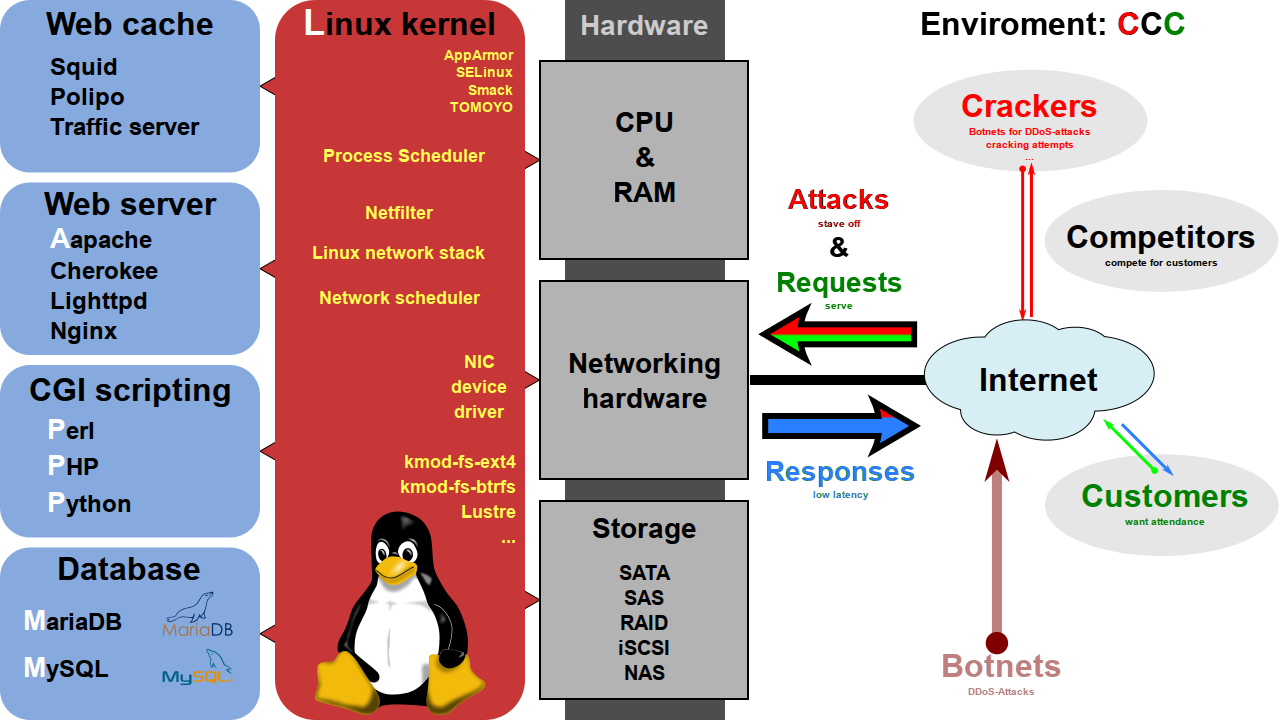
\includegraphics[scale=0.3]{LAMP_software_bundle.png}
\caption{The LAMP Architecture}
\label{LAMP_software_bundle}
\end{figure}

Broad overview of the LAMP software bundle, displayed here together with Squid. A high-performance and high-availability web server solution providing security in a hostile environment.

As of April 2007, over 20 million Internet domains had web services hosted on servers with PHP installed and \textcolor{Blue}{\texttt{mod\_php}} was recorded as the most popular Apache HTTP Server module.[94] PHP is used as the server-side programming language on 75\% of all websites whose server-side programming language is known, and PHP is the most-used open source software within enterprises. Web content management systems written in PHP include MediaWiki, Joomla, eZ Publish, SilverStripe, WordPress, Drupal, Moodle, the user-facing portion of Facebook, and Digg.

For specific and more advanced usage scenarios, PHP offers a well defined and documented way for writing custom extensions in C or C++. Besides extending the language itself in form of additional libraries, extensions are providing a way for improving execution speed where it is critical and there is room for improvements by using a true compiled language. PHP also offers well defined ways for embedding itself into other software projects. That way PHP can be easily used as an internal scripting language for another project, also providing tight interfacing with the project's specific internal data structures.

PHP是一个应用范围很广的语言,特别是在网络程序开发方面。一般来说PHP大多在服务器端运行,通过运行PHP的代码来产生网页提供浏览器读取,此外也可以用来开发命令行脚本程序和用户端的GUI应用程序。

PHP可以在许多的不同种的服务器、操作系统、平台上运行,也可以和许多数据库系统结合。使用PHP不需要任何费用,官方组织PHP Group提供了完整的程序源代码,允许用户修改、编译、扩充来使用。




\section{Frameworks}

PHP官方的框架为Zend framework,2005年开始开发至今已经步入成熟期,尽管对于PHP框架的方向业界还有争议,但在实际生产中框架的使用已非常普遍。

另一些常用的PHP框架有:Yii、CodeIgniter、CakePHP、Symfony、QeePHP/FleaPHP、ThinkPHP等,使用这些框架,可以使项目得到更快更简单的部署和更加敏捷的开发效率,但在另一方面,学习这些框架的使用需要付出额外的学习成本。





\section{Libraries}



内置多样化的函数是PHP主要的特点之一,这些开放代码的函数提供了各种不同的功能,例如文件处理、FTP、字符串处理、等等。这些函数的使用方法和C语言相近(例如printf),这也是PHP广为流行的原因之一。

除了内置的函数之外,PHP也提供了很多扩展库(extension),像是各种数据库连接函数、数据压缩函数、图形处理等等。有些延伸库需要从PECL(PHP Extension Community Library)取得。

以下是PHP编程语言提供的库列表。



\begin{table}
\centering
\caption{PHP Libraries}
\label{php_libraries}
\rowcolors{1}{White}{Lavender}
\begin{tabular}{m{65pt}m{135pt}m{90pt}m{80pt}}
Apache			&Gettext						&mSQL			&SESAM\\
BCMath			&GD Graphics Library			&MySQL		&Session Handling\\
Bzip2			&GNU Multi-Precision Library	&Mowhawk		&Shared memory\\
Calendars		&Hyperwave					&muscat		&SMTP\\
CCVS			&iconv							&Ncurses		&SNMP\\
COM			&IMAP,POP3 and NNTP		&ODBC			&Sockets\\
ClibPDF			&Informix						&Oracle		&SimpleXML\\
cURL			&Ingres II						&OpenSSL		&SQLite\\
Cybercash		&InterBase						&Ovrimos SQL	&Streams\\
DB2			&IRC							&PDF			&Sybase\\
dBase			&LDAP							&PayFlow Pro	&Token\\
DBM			&Lotus Notes					&PDO			&vpopmail\\
dbx				&mailparse						&POSIX			&WDDX\\
DB++			& MCAL							&PostgreSQL	&Win32 API\\
DOM XML		&Mcrypt						&Printer		&XML(Xpath)\\
.NET			&MCVE							&Pspell			&XML-RPC\\
FileMaker Pro	&Mhash							&GNU Readline	&XSLT\\
FrontBase		&MIME Functions				&GNU Recode	&YAZ\\
filePro			& MS-SQL						&Regular expressions&Yellow Pages/NIS\\
FriBiDi			&Ming							&QT-Dom		&ZIP\\
FTP				&mnoGoSearch					&Semaphores	&Zlib\\


\end{tabular}
\end{table}




\chapter{Security}


About 30\% of all vulnerabilities listed on the National Vulnerability Database are linked to PHP. These vulnerabilities are caused mostly by not following best-practice programming rules. Technical security flaws of the language itself or of its core libraries are not frequent (23 in 2008, about 1\% of the total). Recognizing that programmers make mistakes, some languages include taint checking to automatically detect the lack of input validation which induces many issues. Such a feature is being developed for PHP, but its inclusion in a release has been rejected several times in the past.

There are advanced protection patches such as Suhosin and Hardening-Patch, especially designed for web hosting environments.

Some of the vulnerabilities are induced by improper PHP's runtime configuration. For example, failing to disable PHP execution for the directory where uploaded images are stored, can result in execution of malicious PHP code embedded within uploaded images. Another well known example is leaving enabled the dynamic loading of PHP extensions, in a shared hosting environment.

据National Vulnerability Database数据显示,与PHP有关的数据库攻击比例为:20\% 2004, 28\% 2005, 43\% 2006, 36\% 2007, 35\% 2008 and 32\% 2009。其中很多的漏洞都可以通过远程操作完成,黑客可以通过网络连接攻击服务器,达到盗取或毁坏数据,发送垃圾邮件或进行分布式拒绝服务攻击。但是随着更多的关注,PHP也变得越来越安全了。


2010年12月17日,PHP代码“贡献者名单”中被加入“Wolegequ Gelivable”字样(中文含义“我勒个去 给力”),约半小时后被删除。2011年3月19日,PHP官方发布声明指出,黑客可能是通过wiki.php.net作为入口攻击了代码系统。并且,官方已经检查过自版本5.3.5以来发布的代码,并没有发现恶意内容。但官方同时表示,尚未完全掌握黑客发动本次攻击的具体细节。


\section{Thread Safe}

Windows版的PHP从版本5.2.1开始有Thread Safe(线程安全)和None Thread Safe(NTS,非线程安全)之分,这两者不同在于何处\cite{thread_safe}?到底应该用哪种?这里做一个简单的介绍。

从2000年10月20日发布的第一 个Windows版的PHP3.0.17开始的都是线程安全的版本。与Linux/Unix系统是采用多进程的工作方式不同的是,Windows系统的是多线程的工作方式。如果在IIS下以CGI方式运行PHP会非常慢,这是由于CGI模式是建立在多进程的基础之上的,而非多线程。

一般我们会把PHP配置成以ISAPI的方式来运行,ISAPI是多线程的方式,这样就快多了。但存在一个问题,很多常用的PHP扩展是以Linux/Unix的多进程思想来开发的,这些扩展在ISAPI的方式运行时就会出错搞垮IIS,因此在IIS下CGI模式才是PHP运行的最安全方式,但CGI模式对于每个HTTP请求都需要重新加载和卸载整个PHP环境,其消耗是巨大的。

为了兼顾IIS下PHP的效率和安全,微软给出了FastCGI的解决方案。FastCGI可以让PHP的进程重复利用而不是每一个新的请求就重开一个进程,同时FastCGI也可以允许几个进程同时执行。这样既解决了CGI进程模式消耗太大的问题,又利用上了CGI进程模式不存在线程安全问题的优势。

因此,如果是使用ISAPI的方式来运行PHP就必须用Thread Safe(线程安全)的版本;而用FastCGI模式运行PHP的话就没有必要用线程安全检查了,用None Thread Safe(NTS,非线程安全)的版本能够更好的提高效率。

\section{Version}

If you are using PHP with Apache 1 or Apache2 from apache.org you need to use the VC6 versions of PHP

If you are using PHP with IIS you should use the VC9 versions of PHP

VC6 Versions are compiled with the legacy Visual Studio 6 compiler

VC9 Versions are compiled with the Visual Studio 2008 compiler and have improvements in performance and stability. The VC9 versions require you to have the Microsoft 2008 C++ Runtime (x86) or the Microsoft 2008 C++ Runtime (x64) installed

Do NOT use VC9 version with apache.org binaries

VC9 versions of Apache can be fetched at Apache Lounge. We use their binaries to build the Apache SAPIs.







\chapter{Criticism}




PHP has been criticized for its heavy cluttering of main distribution with many functions, case-insensitive function names, among other specific details.


PHP has also been criticized heavily for the security vulnerabilities that can be created by certain language features, induced by some of the historically default values for their associated runtime settings. Among these, magic quotes and \textcolor{Blue}{\texttt{register\_globals}} are the best known. The latter made any URL parameters become variables, which while making programming easier, could create serious security vulnerabilities as it allowed an attacker to set the value of any variable and interfere with script execution.

It is felt PHP interferes with productivity because the lack of language design introduces unpredictable behavior, inconsistent function naming and parameter usage, dependency on new constructs to work around lower level language quirks, introduction of new constructs with flaky behavior, and missing or inconsistent error handling features.


It also lacks features such as native Unicode support and multithreading at the PHP core level, though using threads is made possible by the pthreads PECL extension.



\bibliographystyle{plainnat}
\bibliography{phpnotes}
\setcitestyle{numbers}

















































































\part{Foundation}

{\CTEXnoindent\textbf{版权信息}}


Copyright © 1997 - 2013,PHP 文档组版权所有。发行本资料必须服从 Creative Commons Attribution 3.0 或更新版许可中阐明的条款及条件。\href{http://www.php.net/manual/zh/cc.license.php}{Creative Commons Attribution 3.0 license} 的副本已随本手册发行。其最新版本位于 »~\url{http://creativecommons.org/licenses/by/3.0/}。

如有兴趣再发行或再版此文档的全部或部分内容,不论修改过与否,或有任何问题,请联系版权所有者 » \href{doc-license@lists.php.net}{doc-license@lists.php.net}。注意,本地址映射到一个公开归档的邮件列表。

{\CTEXnoindent\textbf{作者与贡献者}}

在手册的首页上仅突出了目前最活跃的人员,但还有更多的贡献者正在帮助我们工作或在过去给项目提供过巨大的帮助。有许多不知名的人帮助在手册中写下用户评论,并不断地包含在参考中,也很感谢他们的努力。下面所提供的列表均以字母顺序排序。

{\CTEXnoindent\textbf{作者与编辑}}

下列人员曾经或者目前正在为本手册添砖加瓦: Bill Abt, Jouni Ahto, Alexander Aulbach, Daniel Beckham, Stig Bakken, Nilgün Belma Bugüner, Jesus M. Castagnetto, Ron Chmara, Sean Coates, John Coggeshall, Simone Cortesi, Peter Cowburn, Daniel Egeberg, Markus Fischer, Wez Furlong, Sara Golemon, Rui Hirokawa, Brad House, Pierre-Alain Joye, Etienne Kneuss, Moriyoshi Koizumi, Rasmus Lerdorf, Andrew Lindeman, Stanislav Malyshev, Justin Martin, Rafael Martinez, Rick McGuire, Moacir de Oliveira Miranda Júnior, Kalle Sommer Nielsen, Yasuo Ohgaki, Richard Quadling, Derick Rethans, Rob Richards, Sander Roobol, Egon Schmid, Thomas Schoefbeck, Sascha Schumann, Dan Scott, Masahiro Takagi, Yannick Torres, Michael Wallner, Lars Torben Wilson, Jim Winstead, Jeroen van Wolffelaar 和 Andrei Zmievski.

下列人员对本手册做了相当数量的编辑工作: Stig Bakken, Gabor Hojtsy, Hartmut Holzgraefe 和 Egon Schmid.


{\CTEXnoindent\textbf{用户评论维护者}}

目前最活跃的维护者是: Daniel Brown, Nuno Lopes, Felipe Pena, Thiago Pojda 和 Maciek Sokolewicz.

下列人员为维护用户评论作出了巨大的努力: Mehdi Achour, Daniel Beckham, Friedhelm Betz, Victor Boivie, Jesus M. Castagnetto, Nicolas Chaillan, Ron Chmara, Sean Coates, James Cox, Vincent Gevers, Sara Golemon, Zak Greant, Szabolcs Heilig, Oliver Hinckel, Hartmut Holzgraefe, Etienne Kneuss, Rasmus Lerdorf, Matthew Li, Andrew Lindeman, Aidan Lister, Hannes Magnusson, Maxim Maletsky, Bobby Matthis, James Moore, Philip Olson, Sebastian Picklum, Derick Rethans, Sander Roobol, Damien Seguy, Jason Sheets, Tom Sommer, Jani Taskinen, Yasuo Ohgaki, Jakub Vrana, Lars Torben Wilson, Jim Winstead, Jared Wyles 和 Jeroen van Wolffelaar.

{\CTEXnoindent\textbf{中文翻译外部支持团队}}

PHP手册中文翻译工作是一项长期而又艰巨的工作,为了让这个工作得以持久进行下去,我们组织了 » \href{http://code.google.com/p/phpdoc-zh/}{PHP 手册中文翻译补完计划}。下列人员目前正在参与该计划:codingall.com(赵磊)、cuimuxi(崔玉松)、cztviztor、gaojian1226、HaoHappy(陈浩)、HonestQiao(乔楚)、kendotom、lgg860911、loosen.copen、miusun01(李鼎峰)、ping3608、r.anerg(罗翀)、suppersoft(paris.wang)、fising(王祥中)、wind.golden(陈金)。

\chapter{PHP Syntax}

\vspace{-20pt}


使用了 PHP 的Web页面将被和通常的 HTML 页面一样处理,可以用通常建立 HTML 页面的方法来建立和编辑它们,但是用户无法在浏览器中通过查看源文档的方式来查看 PHP 的源代码 - 而是只能看到 PHP 文件的输出~——即纯粹的 HTML。这是因为在结果返回浏览器之前,脚本就已经在服务器执行了。




PHP 的脚本块\footnote{用 \texttt{<?php} 来表示 PHP 标识符的起始,然后放入 PHP 语句并通过加上一个终止标识符 \texttt{?>} 来退出 PHP 模式,可以根据需要在 HTML 文件中开启或关闭 PHP 模式。}以 \texttt{<?php} 开始,以 \texttt{?>} 结束,可以把 PHP 的脚本块放置在文档中的任何位置。当然,在支持简写的服务器上,可以使用 \texttt{<?} 和 \texttt{?>} 来开始和结束脚本块。不过,为了达到最好的兼容性,推荐使用标准形式 (\texttt{<?php}),而不是简写形式。

\begin{lstlisting}[language=PHP]
<?php
  ...
?>
\end{lstlisting}

PHP 文件通常会包含 HTML 标签,就像一个 HTML 文件,以及一些 PHP 脚本代码。

在Web服务器根目录(DOCUMENT\_ROOT)下建立一个文件名为 hello.php,然后完成如下内容,它可以向浏览器输出文本 "Hello World":

\begin{lstlisting}[language=HTML]
<!DOCTYPE html>
<html>
<head>
  <title>PHP Example</title>
</head>
<body>
<?php
  echo "Hello World";
?>
</body>
</html>
\end{lstlisting}

在浏览器的地址栏里输入 web 服务器的 URL 访问这个文件,在结尾加上“/hello.php”。如果本地开发,那么这个 URL 一般是 http://localhost/hello.php 或者 http://127.0.0.1/hello.php,当然这取决于 web 服务器的设置。如果所有的设置都正确,那么这个文件将被 PHP 解析,浏览器中将会输出如下结果:

\begin{lstlisting}[language=HTML]
<!DOCTYPE html>
<html>
 <head>
  <title>PHP Example</title>
 </head>
 <body>
 <p>Hello World</p>
 </body>
</html>
\end{lstlisting}

该程序非常的简单,它仅仅只是利用了 PHP 的 echo 语句显示了 Hello World。注意,这个范例和其它用 C 或 Perl 语言写的脚本之间的区别~——与用大量的命令来编写程序以输出 HTML 不同的是,PHP 页面就是 HTML,只不过在其中嵌入了一些代码来做一些事情,PHP文件无需被执行或以任何方式指定。服务器会找到该文件并提供给 PHP 进行解释,因为使用了“.php”的扩展名,服务器已被配置成自动传递有着“.php”扩展名的文件给 PHP。

{\CTEXnoindent\textbf{PHP结束符}}

PHP 中的每个代码行都必须以分号\footnote{分号是一种分隔符,用于把指令集区分开来。}结束。



有两种通过 PHP 来输出文本的基础指令:echo 和 print。在上面的例子中就是使用echo 语句来输出文本 "Hello World"。

下面建立一个最著名的 PHP 脚本,调用函数 \texttt{phpinfo()},将会看到很多有关自己系统的有用信息,例如预定义变量、已经加载的 PHP 模块和配置信息。

\begin{lstlisting}[language=HTML]
<!DOCTYPE html>
<html>
<head>
  <title>PHP Example</title>
</head>
<body>
<?php
  phpinfo();
?>
</body>
</html>
\end{lstlisting}

尽管换行在 HTML 中的实际意义不是很大,但适当地使用换行可以使 HTML 代码易读且美观。PHP 会在输出时自动删除其结束符 \texttt{?>} 后的一个换行。该功能主要是针对在一个页面中嵌入多段 PHP 代码或者包含了无实质性输出的 PHP 文件而设计,与此同时也造成了一些疑惑。如果需要在 PHP 结束符 \texttt{?>}之后输出换行的话,可以在其后加一个空格,或者在最后的一个 echo/print 语句中加入一个换行。



{\CTEXnoindent\textbf{PHP注释}}

与C/C++/C\#/Java 等语言一样,PHP使用 \texttt{//} 来编写单行注释,或者使用 \texttt{/*} 和 \texttt{*/} 来编写大的注释块。


\begin{lstlisting}[language=HTML]
<!DOCTYPE html>
<html>
<head>
<title></title>
</head>
<body>

<?php

//This is a comment

/*
This is
a comment
block
*/

?>

</body>
</html>
\end{lstlisting}

和客户端的 JavaScript 不同的是,PHP 代码是运行在服务端的。如果在服务器上建立了如上例类似的代码,则在运行该脚本后,客户端就能接收到其结果,但他们无法得知其背后的代码是如何运作的。甚至可以将 web 服务器设置成让 PHP 来处理所有的 HTML 文件,这么一来,用户就无法得知服务端到底做了什么。

如果希望用文本编辑工具\footnote{如果使用 Windows 记事本来编写 PHP 脚本,需要注意在保存文件时,文件的后缀名应该为 .php(记事本将自动在文件名后面加上 .txt 后缀,除非采取以下措施之一来避免这种情况)。当保存文件时,系统会提示指定文件的文件名,这时需要将文件名加上引号(例如 ``hello.php")。或者,也可以点击“另存为”对话框中的“保存类型”下拉菜单,并将设置改为“所有文件”。这样在输入文件名的时候就不用加引号了。}来处理PHP脚本,必须保证将结果存成了纯文本格式,否则 PHP 将无法读取并运行这些脚本。



\chapter{PHP Variable}






PHP 中的所有变量都是以 \texttt{\$} 符号开始的,变量用于存储值,比如数字、字符串或函数的结果,这样我们就可以在脚本中多次使用它们了。与C++等不同的是,不需要在变量使用前确定该变量的类型,而是由所赋的值所决定。


在决定了一个变量的类型后,不要轻易改动,以免发生错误,下面是在 PHP 中设置变量的语法:

\begin{lstlisting}[language=PHP]
$var_name = value;
\end{lstlisting}



如果忘记在变量的前面的 \texttt{\$} 符号的话,变量将是无效的。下面将创建一个存有字符串的变量,和一个存有数值的变量:


\begin{lstlisting}[language=PHP]
<?php
$txt = "Hello World!";
$number = 16;
?>
\end{lstlisting}


PHP 是一门松散类型的语言(Loosely Typed Language),不需要在设置变量之前声明该变量,也不必向 PHP 声明该变量的数据类型,根据变量被设置的方式,PHP 会自动地把变量转换为正确的数据类型。

在强类型的编程语言中,必须在使用前声明变量的类型和名称,而在 PHP 中,变量会在使用时被自动声明。

PHP中变量的命名规则如下:

\begin{compactitem}
\item 变量名必须以字母或下划线 "\_" 开头。
\item 变量名只能包含字母数字字符以及下划线。
\item 变量名不能包含空格。如果变量名由多个单词组成,那么应该使用下划线进行分隔(比如 \texttt{\$my\_string}),或者以大写字母开头(比如 \texttt{\$myString})。
\end{compactitem}


\chapter{PHP String}


PHP中的字符串变量用于包含字符串的值,存储并处理文本片段。同时,PHP提供了很多的字符串函数供用户对字符串进行操作,从而更加灵活的处理字符串,而且PHP字符串函数是 PHP 核心的组成部分,无需安装即可使用这些函数。


在创建字符串之后就可以对它进行操作了,可以直接在函数中使用字符串,或者把它存储在变量中,比如在下面的例子中,PHP 脚本把字符串 "Hello World" 赋值给名为 \texttt{\$txt} 的字符串变量:


\begin{lstlisting}[language=PHP]
<?php
$txt="Hello World";
echo $txt;
?>
\end{lstlisting}


以上代码的输出:\verb|Hello World|


\section{Concatenation Operator}



在 PHP 中,只有一个字符串运算符,称为并置运算符 (\texttt{.}),用于把两个字符串值连接起来。

要把两个变量连接在一起,可以使用这个点运算符 (.) :

\begin{lstlisting}[language=PHP]
<?php
  $txt1="Hello World";
  $txt2="1234";
  echo $txt1 . " " . $txt2;
?>
\end{lstlisting}


以上代码的输出:\verb|Hello World 1234|


在上面的例子中使用了两次并置运算符,这是由于我们需要插入第三个字符串。为了分隔这两个变量,我们在 \$txt1 与 \$txt2 之间插入了一个空格。


\section{strlen()}


strlen() 函数用于计算字符串的长度,下面的示例中使用strlen()来计算出字符串 "Hello world!" 的长度:

\begin{lstlisting}[language=PHP]
<?php
  echo strlen("Hello world!");
?>
\end{lstlisting}


以上代码的输出:\verb|12|

字符串的长度信息常常用在循环或其他函数中,因为那时确定字符串何时结束是很重要的(例如,在循环中,我们需要在字符串中的最后一个字符之后结束循环)。

\section{strpos()}

strpos() 函数用于在字符串内检索一段字符串或一个字符。如果在字符串中找到匹配,该函数会返回第一个匹配的位置。如果未找到匹配,则返回 FALSE。

下面的示例演示如何在字符串中找到子字符串 "world":



\begin{lstlisting}[language=PHP]
<?php
  echo strpos("Hello world!", "world");
?>
\end{lstlisting}

以上代码的输出是:\verb|6|

在字符串"Hello world!"中,字符串 "world" 的位置是 6,至于返回 6 而不是 7,是由于字符串中的首个位置是 0,而不是 1。


\section{PHP String Functions}



\begin{longtable}{|m{120pt}|m{250pt}|m{20pt}|}
%head
\multicolumn{3}{r}{}
\tabularnewline\hline
函数	&描述	&PHP
\endhead
%endhead

%firsthead
\caption{PHP String 函数}\\
\hline
函数	&描述	&PHP
\endfirsthead
%endfirsthead

%foot
\multicolumn{3}{r}{}
\endfoot
%endfoot

%lastfoot
\endlastfoot
%endlastfoot

\hline
addcslashes()				&在指定的字符前添加反斜杠。	&4\\
\hline
addslashes()				&在指定的预定义字符前添加反斜杠。&	3\\
\hline
bin2hex()					&把 ASCII 字符的字符串转换为十六进制值。&	3\\
\hline
chop()						&rtrim() 的别名。	&3\\
\hline
chr()						&从指定的 ASCII 值返回字符。&	3\\
\hline
chunk\_split()				&把字符串分割为一连串更小的部分。&	3\\
\hline
convert\_cyr\_string()		&把字符由一种 Cyrillic 字符转换成另一种。&	3\\
\hline
convert\_uudecode()			&对 uuencode 编码的字符串进行解码。	&5\\
\hline
convert\_uuencode()			&使用 uuencode 算法对字符串进行编码。&	5\\
\hline
count\_chars()				&返回字符串所用字符的信息。	&4\\
\hline
crc32()						&计算一个字符串的 32-bit CRC。&	4\\
\hline
crypt()						&单向的字符串加密法 (hashing)。&	3\\
\hline
echo()						&输出字符串。	&3\\
\hline
explode()					&把字符串打散为数组。&	3\\
\hline
fprintf()						&把格式化的字符串写到指定的输出流。&	5\\
\hline
get\_html\_translation\_table()&返回翻译表。	&4\\
\hline
hebrev()					&把希伯来文本从右至左的流转换为左至右的流。	&3\\
\hline
hebrevc()					&同上,同时把({\textbackslash}n) 转为	<br />。	&3\\
\hline
html\_entity\_decode()		&把 HTML 实体转换为字符。	&4\\
\hline
htmlentities()				&把字符转换为 HTML 实体。&	3\\
\hline
htmlspecialchars\_decode()	&把一些预定义的 HTML 实体转换为字符。&	5\\
\hline
htmlspecialchars()			&把一些预定义的字符转换为 HTML 实体。&	3\\
\hline
implode()					&把数组元素组合为一个字符串。	&3\\
\hline
join()						&implode() 的别名。	&3\\
\hline
levenshtein()				&返回两个字符串之间的 Levenshtein 距离。&	3\\
\hline
localeconv()					&返回包含本地数字及货币信息格式的数组。&	4\\
\hline
ltrim()						&从字符串左侧删除空格或其他预定义字符。&	3\\
\hline
md5()						&计算字符串的 MD5 散列。	&3\\
\hline
md5\_file()					&计算文件的 MD5 散列。	&4\\
\hline
metaphone()				&计算字符串的 metaphone 键。&	4\\
\hline
money\_format()				&把字符串格式化为货币字符串。&	4\\
\hline
nl\_langinfo()				&返回指定的本地信息。	&4\\
\hline
nl2br()						&在字符串中的每个新行之前插入 HTML 换行符。	&3\\
\hline
number\_format()			&通过千位分组来格式化数字。	&3\\
\hline
ord()						&返回字符串第一个字符的 ASCII 值。&	3\\
\hline
parse\_str()					&把查询字符串解析到变量中。	&3\\
\hline
print()						&输出一个或多个字符串。	&3\\
\hline
printf()						&输出格式化的字符串。	&3\\
\hline
quoted\_printable\_decode()	&解码 quoted-printable 字符串。&	3\\
\hline
quotemeta()				&在字符串中某些预定义的字符前添加反斜杠。	&3\\
\hline
rtrim()						&从字符串的末端开始删除空白字符或其他预定义字符。	&3\\
\hline
setlocale()					&设置地区信息(地域信息)。	&3\\
\hline
sha1()						&计算字符串的 SHA-1 散列。	&4\\
\hline
sha1\_file()					&计算文件的 SHA-1 散列。	&4\\
\hline
similar\_text()				&计算两个字符串的匹配字符的数目。	&3\\
\hline
soundex()					&计算字符串的 soundex 键。	&3\\
\hline
sprintf()					&把格式化的字符串写写入一个变量中。	&3\\
\hline
sscanf()						&根据指定的格式解析来自一个字符串的输入。	&4\\
\hline
str\_ireplace()				&替换字符串中的一些字符。\newline(对大小写不敏感)	&5\\
\hline
str\_pad()					&把字符串填充为新的长度。	&4\\
\hline
str\_repeat()				&把字符串重复指定的次数。	&4\\
\hline
str\_replace()				&替换字符串中的一些字符。\newline(对大小写敏感)	&3\\
\hline
str\_rot13()					&对字符串执行 ROT13 编码。	&4\\
\hline
str\_shuffle()				&随机地打乱字符串中的所有字符。&	4\\
\hline
str\_split()					&把字符串分割到数组中。	&5\\
\hline
str\_word\_count()			&计算字符串中的单词数。&	4\\
\hline
strcasecmp()				&比较两个字符串。\newline(对大小写不敏感)&	3\\
\hline
strchr()						&搜索字符串在另一字符串中的第一次出现。\newline strstr() 的别名	&3\\
\hline
strcmp()					&比较两个字符串。\newline(对大小写敏感)	&3\\
\hline
strcoll()						&比较两个字符串(根据本地设置)。	&4\\
\hline
strcspn()					&返回在找到任何指定的字符之前,在字符串查找的字符数。&	3\\
\hline
strip\_tags()					&剥去 HTML、XML 以及 PHP 的标签。	&3\\
\hline
stripcslashes()				&删除由 addcslashes() 函数添加的反斜杠。&	4\\
\hline
stripslashes()				&删除由 addslashes() 函数添加的反斜杠。&	3\\
\hline
stripos()					&返回字符串在另一字符串中第一次出现的位置。\newline (大小写不敏感)	&5\\
\hline
stristr()						&查找字符串在另一字符串中第一次出现的位置。\newline (大小写不敏感)	&3\\
\hline
strlen()						&返回字符串的长度。	&3\\
\hline
strnatcasecmp()				&使用一种“自然”算法来比较两个字符串。\newline(对大小写不敏感)&	4\\
\hline
strnatcmp()					&使用一种“自然”算法来比较两个字符串。\newline(对大小写敏感)	&4\\
\hline
strncasecmp()				&前 n 个字符的字符串比较。\newline(对大小写不敏感)。	&4\\
\hline
strncmp()					&前 n 个字符的字符串比较。\newline(对大小写敏感)。&	4\\
\hline
strpbrk()					&在字符串中搜索指定字符中的任意一个。	&5\\
\hline
strpos()					&返回字符串在另一字符串中首次出现的位置。\newline(对大小写敏感)&	3\\
\hline
strrchr()					&查找字符串在另一个字符串中最后一次出现的位置。	&3\\
\hline
strrev()						&反转字符串。	&3\\
\hline
strripos()					&查找字符串在另一字符串中最后出现的位置。\newline (对大小写不敏感)	&5\\
\hline
strrpos()					&查找字符串在另一字符串中最后出现的位置。\newline (对大小写敏感)	&3\\
\hline
strspn()						&返回在字符串中包含的特定字符的数目。	&3\\
\hline
strstr()						&搜索字符串在另一字符串中的首次出现。\newline(对大小写敏感)	&3\\
\hline
strtok()						&把字符串分割为更小的字符串。	&3\\
\hline
strtolower()				&把字符串转换为小写。	&3\\
\hline
strtoupper()				&把字符串转换为大写。&	3\\
\hline
strtr()						&转换字符串中特定的字符。&	3\\
\hline
substr()						&返回字符串的一部分。	&3\\
\hline
substr\_compare()			&从指定的开始长度比较两个字符串。	&5\\
\hline
substr\_count()				&计算子串在字符串中出现的次数。	&4\\
\hline
substr\_replace()			&把字符串的一部分替换为另一个字符串。&	4\\
\hline
trim()						&从字符串的两端删除空白字符和其他预定义字符。&	3\\
\hline
ucfirst()						&把字符串中的首字符转换为大写。	&3\\
\hline
ucwords()					&把字符串中每个单词的首字符转换为大写。&	3\\
\hline
vfprintf()					&把格式化的字符串写到指定的输出流。	&5\\
\hline
vprintf()					&输出格式化的字符串。	&4\\
\hline
vsprintf()					&把格式化字符串写入变量中。&	4\\
\hline
wordwrap()					&按照指定长度对字符串进行折行处理。&	4\\
\hline
\end{longtable}


\section{PHP String Constants}





\begin{longtable}{|m{120pt}|m{250pt}|m{20pt}|}
%head
\multicolumn{3}{r}{}
\tabularnewline\hline
常量	&描述	&PHP
\endhead
%endhead

%firsthead
\caption{PHP String 常量}\\
\hline
常量	&描述	&PHP
\endfirsthead
%endfirsthead

%foot
\multicolumn{3}{r}{}
\endfoot
%endfoot

%lastfoot
\endlastfoot
%endlastfoot

\hline
CRYPT\_SALT\_LENGTH	&包含系统默认加密方法的长度。\newline 对于标准 DES 加密,长度是 2。	 &\\
\hline
CRYPT\_STD\_DES		&如果支持 2 字符 salt 的 DES 加密,则设置为 1,否则为 0。	 &\\
\hline
CRYPT\_EXT\_DES		&如果支持 9 字符 salt 的 DES 加密,则设置为 1,否则为 0。	 &\\
\hline
CRYPT\_MD5			&如果支持以$1$开始的 12 字符 salt 的MD5加密,则设置为1,否则为0。	 &\\
\hline
CRYPT\_BLOWFISH		&如果支持以 $2$ 或 $2a$ 开始的 16 字符 salt 的 Blowfish 加密,则设置为 1,否则为 0。	 &\\
\hline
HTML\_SPECIALCHARS	& 	 &\\
\hline
HTML\_ENTITIES	 	 	&&\\
\hline
ENT\_COMPAT	 	 	&&\\
\hline
ENT\_QUOTES	 	 	&&\\
\hline
ENT\_NOQUOTES	 	& &\\
\hline
CHAR\_MAX	 	 		&&\\
\hline
LC\_CTYPE	 	 		&&\\
\hline
LC\_NUMERIC	 	 	&&\\
\hline
LC\_TIME	 	 		&&\\
\hline
LC\_COLLATE	 	 	&&\\
\hline
LC\_MONETARY	 	 	&&\\
\hline
LC\_ALL	 	 			&&\\
\hline
LC\_MESSAGES	 	 	&&\\
\hline
STR\_PAD\_LEFT	 	 	&&\\
\hline
STR\_PAD\_RIGHT	 	& &\\
\hline
STR\_PAD\_BOTH	 	&&\\
\hline
\end{longtable}



\chapter{PHP Operators}

PHP的运算符包括\verb|+ - * / > < >= <=|等,与C++十分类似。


\section{Arithmetic Operators}

\begin{longtable}{|m{35pt}|m{180pt}|m{80pt}|m{30pt}|}
%head
\multicolumn{4}{r}{}
\tabularnewline\hline
运算符	&说明	&示例	&结果
\endhead
%endhead

%firsthead
\caption{PHP 算术运算符}\\
\hline
运算符	&说明	&示例	&结果
\endfirsthead
%endfirsthead

%foot
\multicolumn{4}{r}{}
\endfoot
%endfoot

%lastfoot
\endlastfoot
%endlastfoot
\hline
+	&Addition		&x=2 \newline x+2		&4\\
\hline
-	&Subtraction	&x=2 \newline 5-x		&3\\
\hline
*	&Multiplication	&x=4 \newline x*5		&20\\
\hline
/	&Division		&15/5 \newline 5/2		&3 \newline 2.5\\
\hline
\%	&Modulus (division remainder)	&5\%2 \newline 10\%8 \newline 10\%2	&1 \newline 2 \newline 0\\
\hline
++	&Increment		& x=5 \newline x++	 &x=6\\
\hline
-\/-	&Decrement	&x=5 \newline x-\/-	&x=4\\
\hline

\end{longtable}



\section{Assignment Operators}

\begin{longtable}{|m{35pt}|m{180pt}|m{80pt}|m{30pt}|}
%head
\multicolumn{4}{r}{}
\tabularnewline\hline
运算符	&说明	&示例	&结果
\endhead
%endhead

%firsthead
\caption{PHP 赋值运算符}\\
\hline
运算符	&说明	&示例	&结果
\endfirsthead
%endfirsthead

%foot
\multicolumn{4}{r}{}
\endfoot
%endfoot

%lastfoot
\endlastfoot
%endlastfoot
\hline
=		&x=y		&x=y&\\
\hline
+\/=	&x+\/=y	&x=x+y&\\
\hline
-\/=		&x-\/=y		&x=x-y&\\
\hline
*\/=	&x*\/=y	&x=x*y&\\
\hline
/\/=		&x/\/=y		&x=x/y&\\
\hline
.\/=		&x.\/=y		&x=x.y&\\
\hline
\%\/=	&x\%\/=y	&x=x\%y&\\
\hline
\end{longtable}



\section{Comparison Operators}


\begin{longtable}{|m{35pt}|m{180pt}|m{80pt}|m{30pt}|}
%head
\multicolumn{4}{r}{}
\tabularnewline\hline
运算符	&说明	&示例	&结果
\endhead
%endhead

%firsthead
\caption{PHP 比较运算符}\\
\hline
运算符	&说明	&示例	&结果
\endfirsthead
%endfirsthead

%foot
\multicolumn{4}{r}{}
\endfoot
%endfoot

%lastfoot
\endlastfoot
%endlastfoot
\hline
=\/=	&is equal to					&5==8 returns false&false\\
\hline
!\/=	&is not equal					&5!=8 returns true&true\\
\hline
>	&is greater than					&5>8 returns false&false\\
\hline
<	&is less than					&5<8 returns true&true\\
\hline
>\/=	&is greater than or equal to &5>=8 returns false&false\\
\hline
<\/=	&is less than or equal to	&5<=8 returns true&true\\
\hline

\end{longtable}


\section{Logical Operators}



\begin{longtable}{|m{35pt}|m{60pt}|m{200pt}|m{30pt}|}
%head
\multicolumn{4}{r}{}
\tabularnewline\hline
运算符	&说明	&示例	&结果
\endhead
%endhead

%firsthead
\caption{PHP 逻辑运算符}\\
\hline
运算符	&说明	&示例	&结果
\endfirsthead
%endfirsthead

%foot
\multicolumn{4}{r}{}
\endfoot
%endfoot

%lastfoot
\endlastfoot
%endlastfoot
\hline
\&\&	&and	 				&x=6 \newline y=3 \newline (x < 10 \&\& y > 1) returns true&true\\
\hline
||		&or	 					& x=6 \newline y=3 \newline (x==5 || y==5) returns false&false\\
\hline
!		&not	 				& x=6 \newline y=3 \newline !(x==y) returns true		&true\\
\hline
\end{longtable}





\chapter{PHP Statements}

if、elseif 以及 else 语句用于执行基于不同条件的不同动作。



\section{Conditional statements}

编写代码时,常常需要为不同的判断执行不同的动作,这时可以在代码中使用条件语句来完成此任务。

\begin{compactitem}
\item if...else

在条件成立时执行一块代码,条件不成立时执行另一块代码

\item elseif

与 if...else 配合使用,在若干条件之一成立时执行一个代码块
\end{compactitem}



\subsection{if...else statements}

如果希望在某个条件成立时执行一些代码,在条件不成立时执行另一些代码,使用 if....else 语句。

\begin{lstlisting}[language=PHP]
if (condition)
  code to be executed if condition is true;
else
  code to be executed if condition is false; 
\end{lstlisting}


如果当前日期是周五,下面的代码将输出 "Have a nice weekend!",否则会输出 "Have a nice day!":


\begin{lstlisting}[language=PHP]
<!DOCTYPE html>
<html>
<head>
<title></title>
</head>
<body>

<?php
$d=date("D");
if ($d=="Fri")
  echo "Have a nice weekend!"; 
else
  echo "Have a nice day!"; 
?>

</body>
</html>
\end{lstlisting}

如果需要在条件成立或不成立时执行多行代码,应该把这些代码行包括在花括号中:

\begin{lstlisting}[language=PHP]
<!DOCTYPE html>
<html>
<head>
<title></title>
</head>
<body>

<?php
$d=date("D");
if ($d=="Fri")
  {
  echo "Hello!<br />"; 
  echo "Have a nice weekend!";
  echo "See you on Monday!";
  }
?>

</body>
</html>
\end{lstlisting}


\subsection{elseif statements}


如果希望在多个条件之一成立时执行代码,使用 elseif 语句:

\begin{lstlisting}[language=PHP]
if (condition)
  code to be executed if condition is true;
elseif (condition)
  code to be executed if condition is true;
else
  code to be executed if condition is false; 
\end{lstlisting}

如果当前日期是周五,下面的例子会输出 "Have a nice weekend!",如果是周日,则输出 "Have a nice Sunday!",否则输出 "Have a nice day!":

\begin{lstlisting}[language=PHP]
<!DOCTYPE html>
<html>
<head>
<title></title>
</head>
<body>

<?php
$d=date("D");
if ($d=="Fri")
  echo "Have a nice weekend!"; 
elseif ($d=="Sun")
  echo "Have a nice Sunday!"; 
else
  echo "Have a nice day!"; 
?>

</body>
</html>
\end{lstlisting}



\section{Select statements}

PHP 中的switch 语句用于执行基于多个不同条件的不同动作,通过switch语句可以可以避免冗长的 if..elseif..else 代码块,从而有选择地执行若干代码块之一。


\subsection{switch...case...default statements}



\begin{lstlisting}[language=PHP]
switch (expression)
{
case label1:
  code to be executed if expression = label1;
  break;  
case label2:
  code to be executed if expression = label2;
  break;
default:
  code to be executed
  if expression is different 
  from both label1 and label2;
}
\end{lstlisting}

switch语句的工作原理如下:

\begin{compactenum}
\item 对表达式(通常是变量)进行一次计算
\item 把表达式的值与结构中 case 的值进行比较
\item 如果存在匹配,则执行与 case 关联的代码
\item 代码执行后,break 语句阻止代码跳入下一个 case 中继续执行
\item 如果没有 case 为真,则使用 default 语句
\end{compactenum}


\begin{lstlisting}[language=PHP]
<!DOCTYPE html>
<html>
<head>
<title></title>
</head>
<body>
<?php
switch ($x)
{
case 1:
  echo "Number 1";
  break;
case 2:
  echo "Number 2";
  break;
case 3:
  echo "Number 3";
  break;
default:
  echo "No number between 1 and 3";
}
?>

</body>
</html>
\end{lstlisting}

\section{Loop statements}



在编写代码时,经常需要让相同的代码块运行很多次,可以在代码中使用循环语句来完成这个任务。


PHP 中的循环语句用于执行相同的代码块指定的次数,循环语句的种类包括:


\begin{compactitem}
\item while - 只要指定的条件成立,则循环执行代码块
\item do...while - 首先执行一次代码块,然后在指定的条件成立时重复这个循环
\item for - 循环执行代码块指定的次数
\item foreach - 根据数组中每个元素来循环代码块
\end{compactitem}



\subsection{while statements}

只要指定的条件成立,while 语句将重复执行代码块。


\begin{lstlisting}[language=PHP]
while (condition)
code to be executed;
\end{lstlisting}

下面的例子示范了一个循环,只要变量 i 小于或等于 5,代码就会一直循环执行下去。循环每循环一次,变量就会递增 1:

\begin{lstlisting}[language=PHP]
<!DOCTYPE html>
<html>
<head>
<title></title>
</head>
<body>

<?php 
$i=1;
while($i<=5)
  {
  echo "The number is " . $i . "<br />";
  $i++;
  }
?>

</body>
</html>
\end{lstlisting}


\subsection{do...while statements}

do...while 语句会至少执行一次代码 - 然后,只要条件成立,就会重复进行循环。

\begin{lstlisting}[language=PHP]
do
{
  code to be executed;
}
while (condition); 
\end{lstlisting}

下面的例子将对 i 的值进行一次累加,然后,只要 i 小于 5 的条件成立,就会继续累加下去:

\begin{lstlisting}[language=PHP]
<!DOCTYPE html>
<html>
<head>
<title></title>
</head>
<body>

<?php 
$i=0;
do {
  $i++;
  echo "The number is " . $i . "<br />";
}
while ($i<5);
?>

</body>
</html>
\end{lstlisting}

\subsection{for statements}

如果已经确定了代码块的重复执行次数,则可以使用 for 语句。

\begin{lstlisting}[language=PHP]
for (initialization; condition; increment)
{
  code to be executed;
}
\end{lstlisting}

for 语句有三个参数。第一个参数初始化变量,第二个参数保存条件,第三个参数包含执行循环所需的增量。如果 initialization 或 increment 参数中包括了多个变量,需要用逗号进行分隔。而条件必须计算为 true 或者 false。

\begin{lstlisting}[language=PHP]
for (initialization; condition; increment)
{
  code to be executed;
}
\end{lstlisting}

下面的例子会把文本 "Hello World!" 显示 5 次:

\begin{lstlisting}[language=PHP]
<!DOCTYPE html>
<html>
<head>
<title></title>
</head>
<body>

<?php
for ($i=1; $i<=5; $i++)
{
  echo "Hello World!<br />";
}
?>

</body>
</html>
\end{lstlisting}

\subsection{foreach statements}

foreach 语句用于循环遍历数组。每进行一次循环,当前数组元素的值就会被赋值给 value 变量(数组指针会逐一地移动) - 以此类推。


\begin{lstlisting}[language=PHP]
foreach (array as value)
{
    code to be executed;
}
\end{lstlisting}

下面的例子示范了一个循环,这个循环可以输出给定数组的值:

\begin{lstlisting}[language=PHP]
<!DOCTYPE html>
<html>
<head>
<title></title>
</head>
<body>

<?php
$arr=array("one", "two", "three");

foreach ($arr as $value)
{
  echo "Value: " . $value . "<br />";
}
?>

</body>
</html>
\end{lstlisting}





\chapter{PHP Array}



在使用 PHP 进行开发的过程中,或早或晚,都会需要创建许多相似的变量,通过PHP数组就能够在单独的变量名中存储一个或多个值。

在PHP中,定义数组会用到array关键字,同时数组是可以定义索引的,方便快捷查询。

数组中的元素都有自己的 ID,因此可以方便地访问它们,PHP有三种数组类型:

\begin{compactitem}
\item 数值数组 - 带有数字 ID 键的数组

\item 关联数组 - 数组中的每个 ID 键关联一个值

\item 多维数组 - 包含一个或多个数组的数组
\end{compactitem}






\section{Numeric array}

数值数组存储的每个元素都带有一个数字 ID 键,可以使用不同的方法来创建数值数组:

\begin{compactenum}
\item[I] 自动分配 ID 键

\begin{lstlisting}[language=PHP]
$names = array("Peter","Quagmire","Joe");
\end{lstlisting}

\item[II] 人工分配ID 键

\begin{lstlisting}[language=PHP]
$names[0] = "Peter";
$names[1] = "Quagmire";
$names[2] = "Joe";
\end{lstlisting}

可以在脚本中使用这些 ID 键:


\begin{lstlisting}[language=PHP]
<?php

$names[0] = "Peter";
$names[1] = "Quagmire";
$names[2] = "Joe";

echo $names[1] . " and " . $names[2] . " are ". $names[0] . "'s neighbors";
?>
\end{lstlisting}


\end{compactenum}





\section{Associative array}


关联数组,它的每个 ID 键都关联一个值。在存储有关具体命名的值的数据时,使用数值数组不是最好的做法。

通过关联数组,我们可以把值作为键,并向它们赋值。

在下面的示例中,使用一个数组把年龄分配给不同的人:


\begin{lstlisting}[language=PHP]
$ages = array("Peter"=>32, "Quagmire"=>30, "Joe"=>34);
\end{lstlisting}

本例与上面相同,不过展示了另一种创建数组的方法:

\begin{lstlisting}[language=PHP]
$ages['Peter'] = "32";
$ages['Quagmire'] = "30";
$ages['Joe'] = "34";
\end{lstlisting}



可以在脚本中使用 ID 键:

\begin{lstlisting}[language=PHP]
<?php

$ages['Peter'] = "32";
$ages['Quagmire'] = "30";
$ages['Joe'] = "34";

echo "Peter is " . $ages['Peter'] . " years old.";
?>
\end{lstlisting}

\section{Multidimensional array}



在多维数组中,主数组中的每个元素也是一个数组。在子数组中的每个元素也可以是数组,以此类推。


下面的示例中创建了一个带有自动分配的 ID 键的多维数组:


\begin{lstlisting}[language=PHP]
$families = array
(
  "Griffin"=>array
  (
  "Peter",
  "Lois",
  "Megan"
  ),
  "Quagmire"=>array
  (
  "Glenn"
  ),
  "Brown"=>array
  (
  "Cleveland",
  "Loretta",
  "Junior"
  )
);
\end{lstlisting}

如果输出这个数组的话,应该类似这样:


\begin{lstlisting}[language=PHP]
Array
(
[Griffin] => Array
  (
  [0] => Peter
  [1] => Lois
  [2] => Megan
  )
[Quagmire] => Array
  (
  [0] => Glenn
  )
[Brown] => Array
  (
  [0] => Cleveland
  [1] => Loretta
  [2] => Junior
  )
)
\end{lstlisting}

如果要显示上面的数组中的一个单一的值:


\begin{lstlisting}[language=PHP]
echo "Is " . $families['Griffin'][2] . " a part of the Griffin family?"; 
\end{lstlisting}





\section{PHP Array Functions}


PHP array 函数允许用户对数组进行操作,而且PHP 支持单维和多维的数组,同时提供了用数据库查询结果来构造数组的函数。

PHP array 函数是 PHP 核心的组成部分,无需安装即可使用这些函数。



\begin{longtable}{|m{120pt}|m{250pt}|m{20pt}|}
%head
\multicolumn{3}{r}{}
\tabularnewline\hline
函数	&描述	&PHP
\endhead
%endhead

%firsthead
\caption{PHP Array 函数}\\
\hline
函数	&描述	&PHP
\endfirsthead
%endfirsthead

%foot
\multicolumn{3}{r}{}
\endfoot
%endfoot

%lastfoot
\endlastfoot
%endlastfoot

\hline
array()							&创建数组。	&3\\
\hline
array\_change\_key\_case()		&返回其键均为大写或小写的数组。	&4\\
\hline
array\_chunk()					&把一个数组分割为新的数组块。	&4\\
\hline
array\_combine()				&通过合并两个数组来创建一个新数组。	&5\\
\hline
array\_count\_values()			&用于统计数组中所有值出现的次数。	&4\\
\hline
array\_diff()						&返回两个数组的差集数组。	&4\\
\hline
array\_diff\_assoc()				&比较键名和键值,并返回两个数组的差集数组。	&4\\
\hline
array\_diff\_key()				&比较键名,并返回两个数组的差集数组。	&5\\
\hline
array\_diff\_uassoc()			&通过用户提供的回调函数做索引检查来计算数组的差集。	&5\\
\hline
array\_diff\_ukey()				&用回调函数对键名比较计算数组的差集。	&5\\
\hline
array\_fill()						&用给定的值填充数组。	&4\\
\hline
array\_filter()					&用回调函数过滤数组中的元素。	&4\\
\hline
array\_flip()						&交换数组中的键和值。	&4\\
\hline
array\_intersect()				&计算数组的交集。	&4\\
\hline
array\_intersect\_assoc()		&比较键名和键值,并返回两个数组的交集数组。	&4\\
\hline
array\_intersect\_key()			&使用键名比较计算数组的交集。	&5\\
\hline
array\_intersect\_uassoc()		&带索引检查计算数组的交集,用回调函数比较索引。	&5\\
\hline
array\_intersect\_ukey()			&用回调函数比较键名来计算数组的交集。	&5\\
\hline
array\_key\_exists()				&检查给定的键名或索引是否存在于数组中。&	4\\
\hline
array\_keys()					&返回数组中所有的键名。	&4\\
\hline
array\_map()					&将回调函数作用到给定数组的单元上。	&4	\\
\hline
array\_merge()					&把一个或多个数组合并为一个数组。	&4\\
\hline
array\_merge\_recursive()		&递归地合并一个或多个数组。	&4\\
\hline
array\_multisort()				&对多个数组或多维数组进行排序。&	4\\
\hline
array\_pad()					&用值将数组填补到指定长度。	&4\\
\hline
array\_pop()					&将数组最后一个单元弹出(出栈)。&	4\\
\hline
array\_product()				&计算数组中所有值的乘积。	&5\\
\hline
array\_push()					&将一个或多个单元(元素)压入数组的末尾(入栈)。	&4\\
\hline
array\_rand()					&从数组中随机选出一个或多个元素,并返回。	&4\\
\hline
array\_reduce()					&用回调函数迭代地将数组简化为单一的值。	&4\\
\hline
array\_reverse()				&将原数组中的元素顺序翻转,创建新的数组并返回。	&4\\
\hline
array\_search()					&在数组中搜索给定的值,如果成功则返回相应的键名。	&4\\
\hline
array\_shift()					&删除数组中的第一个元素,并返回被删除元素的值。	&4\\
\hline
array\_slice()					&在数组中根据条件取出一段值,并返回。	&4\\
\hline
array\_splice()					&把数组中的一部分去掉并用其它值取代。	&4\\
\hline
array\_sum()					&计算数组中所有值的和。	&4\\
\hline
array\_udiff()					&用回调函数比较数据来计算数组的差集。	&5\\
\hline
array\_udiff\_assoc()			&带索引检查计算数组的差集,用回调函数比较数据。	&5\\
\hline
array\_udiff\_uassoc()			&带索引检查计算数组的差集,用回调函数比较数据和索引。	&5\\
\hline
array\_uintersect()				&计算数组的交集,用回调函数比较数据。	&5\\
\hline
array\_uintersect\_assoc()		&带索引检查计算数组的交集,用回调函数比较数据。	&5\\
\hline
array\_uintersect\_uassoc()		&带索引检查计算数组的交集,用回调函数比较数据和索引。	&5\\
\hline
array\_unique()					&删除数组中重复的值。	&4\\
\hline
array\_unshift()					&在数组开头插入一个或多个元素。	&4\\
\hline
array\_values()					&返回数组中所有的值。	&4\\
\hline
array\_walk()					&对数组中的每个成员应用用户函数。	&3\\
\hline
array\_walk\_recursive()		&对数组中的每个成员递归地应用用户函数。	&5\\
\hline
arsort()							&对数组进行逆向排序并保持索引关系。	&3\\
\hline
asort()						&对数组进行排序并保持索引关系。	&3\\
\hline
compact()					&建立一个数组,包括变量名和它们的值。&	4\\
\hline
count()						&计算数组中的元素数目或对象中的属性个数。	&3\\
\hline
current()					&返回数组中的当前元素。	&3\\
\hline
each()						&返回数组中当前的键/值对并将数组指针向前移动一步。	&3\\
\hline
end()						&将数组的内部指针指向最后一个元素。	&3\\
\hline
extract()					&从数组中将变量导入到当前的符号表。	&3\\
\hline
in\_array()					&检查数组中是否存在指定的值。	&4\\
\hline
key()						&从关联数组中取得键名。	&3\\
\hline
krsort()						&对数组按照键名逆向排序。	&3\\
\hline
ksort()						&对数组按照键名排序。	&3\\
\hline
list()						&把数组中的值赋给一些变量。&	3\\
\hline
natcasesort()				&用“自然排序”算法对数组进行不区分大小写字母的排序。	&4\\
\hline
natsort()					&用“自然排序”算法对数组排序。	&4\\
\hline
next()						&将数组中的内部指针向前移动一位。&	3\\
\hline
pos()						&current() 的别名。	&3\\
\hline
prev()						&将数组的内部指针倒回一位。&	3\\
\hline
range()						&建立一个包含指定范围的元素的数组。	&3\\
\hline
reset()						&将数组的内部指针指向第一个元素。	&3\\
\hline
rsort()						&对数组逆向排序。	&3\\
\hline
shuffle()					&把数组中的元素按随机顺序重新排列。	&3\\
\hline
sizeof()						&count() 的别名。	&3\\
\hline
sort()						&对数组排序。	&3\\
\hline
uasort()						&使用用户自定义的比较函数对数组中的值进行排序并保持索引关联。	&3\\
\hline
uksort()						&使用用户自定义的比较函数对数组中的键名进行排序。	&3\\
\hline
usort()						&使用用户自定义的比较函数对数组中的值进行排序。	&3\\
\hline
\end{longtable}



\section{PHP Array Constants}




\begin{longtable}{|m{120pt}|m{250pt}|m{20pt}|}
%head
\multicolumn{3}{r}{}
\tabularnewline\hline
常量	&描述	&PHP
\endhead
%endhead

%firsthead
\caption{PHP Array 常量}\\
\hline
常量	&描述	&PHP
\endfirsthead
%endfirsthead

%foot
\multicolumn{3}{r}{}
\endfoot
%endfoot

%lastfoot
\endlastfoot
%endlastfoot

\hline

CASE\_LOWER	&用在 array\_change\_key\_case() 中将数组键名转换成小写字母。&	 \\
\hline
CASE\_UPPER	&用在 array\_change\_key\_case() 中将数组键名转换成大写字母。&	 \\
\hline
SORT\_ASC		&用在 array\_multisort() 函数中,使其升序排列。	 &\\
\hline
SORT\_DESC		&用在 array\_multisort() 函数中,使其降序排列。	 &\\
\hline
SORT\_REGULAR	&用于对对象进行通常比较。	 &\\
\hline
SORT\_NUMERIC	&用于对对象进行数值比较。	 &\\
\hline
SORT\_STRING	&用于对对象进行字符串比较。	 &\\
\hline
SORT\_LOCALE\_STRING	&基于当前区域来对对象进行字符串比较。	&4\\
\hline
COUNT\_NORMAL	 	& &\\
\hline
COUNT\_RECURSIVE	 	& &\\
\hline
EXTR\_OVERWRITE	 	& &\\
\hline
EXTR\_SKIP	 	 &&\\
\hline
EXTR\_PREFIX\_SAME	 	& &\\
\hline
EXTR\_PREFIX\_ALL	 	& &\\
\hline
EXTR\_PREFIX\_INVALID	& 	 &\\
\hline
EXTR\_PREFIX\_IF\_EXISTS	& 	 &\\
\hline
EXTR\_IF\_EXISTS	 	 &&\\
\hline
EXTR\_REFS	 	 &&\\
\hline
\end{longtable}










\bibliographystyle{plainnat}
\bibliography{phpnotes}









































\part{Functions}





\chapter{Introduction}


PHP提供了超过 700 个内建的函数,函数只需被编译一次就可以多次调用,因而PHP的真正威力源自于它的函数。

PHP 支持函数是“第一等公民”,即函数可以被赋值给一个变量(包括用户自定义的或者是内置函数),然后动态调用它。函数可以作为参数传递给其他函数(称为高阶函数),也可以作为函数返回值返回。

具体来说,函数是一种可以在任何被需要的时候执行的代码块,并且函数可以接受一组参数,然后返回操作结果。



PHP 有很多标准的函数和结构,还有一些函数需要和特定地 PHP 扩展模块一起编译,否则在使用它们的时候就会得到一个致命的“未定义函数”错误。

例如,要使用 image 函数中的 imagecreatetruecolor(),需要在编译 PHP 的时候加上 GD 的支持。或者,要使用 mysql\_connect() 函数,就需要在编译 PHP 的时候加上 MySQL 支持。

PHP的核心函数(例如字符串和变量函数)大多已经包含在每个版本的 PHP 中,调用 phpinfo() 或者 get\_loaded\_extensions() 可以得知 PHP 加载了哪些扩展库,而且很多扩展库默认就是有效的。







\section{Function Prototype}



函数的定义又可以称为函数原型,可以使用function声明自定义函数。

\begin{lstlisting}[language=PHP]
<?php
function foo($arg_1, $arg_2, /* ..., */ $arg_n)
{
    echo "Example function.\n";
    return $retval;
}
?>
\end{lstlisting}

函数的原型说明了函数的返回值,或者函数是否直接作用于传递的参数。例如, str\_replace() 函数将返回修改过的字符串,而 usort() 却直接作用于传递的参数变量本身。

\begin{compactitem}
\item 所有的函数都使用关键词``\texttt{function()}" 来开始
\item 命名函数 - 函数的名称应该提示出它的功能,函数名称以字母或下划线开头。
\item 添加``\texttt{\{}" - 开口的花括号之后的部分是函数的代码。
\item 插入函数代码
\item 添加一个``\texttt{\}}" - 函数通过关闭花括号来结束。
\end{compactitem}

函数定义首先会告诉我们函数返回什么类型的值,以及函数有多少个变量。任何有效的 PHP 代码都有可能出现在函数内部,还可以包括其它函数和类定义。


函数名和 PHP 中的其它标识符命名规则相同,即有效的函数名应该以字母或下划线开始,后面跟字母、数字或下划线。

函数名是大小写无关的,不过在调用函数的时候,使用其在定义时相同的形式是个好习惯。

可以用正则表达式将函数名规则表示为:\colorbox{lightgray}{\texttt{[a-zA-Z\_\textbackslash x7f-\textbackslash xff][a-zA-Z0-9\_\textbackslash x7f-\textbackslash xff]*}}。

下面用函数 strlen() 的定义作为第一个范例:

\begin{verbatim}
strlen
(PHP 4, PHP 5)
strlen -- 获取字符串长度
说明
int strlen ( string str )
返回给定的字符串 string 的长度。
\end{verbatim}

\begin{table}
\centering
\caption{函数原型}
\begin{tabular}{|l|l|}
\hline
组成部分	&说明\\
\hline
strlen	 &函数名称。\\
\hline
(PHP 4, PHP 5)	& strlen() 在 PHP 4 和 PHP 5 的所有版本中都存在。\\
\hline
int	 &该函数返回的值的类型,这里为整型 integer(即以数字来衡量的字符串的长度)。\\
\hline
( string str )	 &第一个参数,在该函数中名为 str,且类型为 string。\\
\hline
\end{tabular}
\end{table}

可以将以上函数的定义写成一般形式:

\begin{verbatim}
返回类型          函数名           ( 参数类型          参数名 )
returned type    function name    ( parameter type   parameter name )
\end{verbatim}



很多函数(例如 in\_array())都有多个变量,其函数原型如下:

\begin{verbatim}
 bool in_array ( mixed $needle, array $haystack [, bool $strict])
\end{verbatim}

in\_array() 返回一个“布尔”值,成功(如果在参数 haystack 中能找到参数 needle)则返回 TRUE, 或者在失败时返回 FALSE(如果在参数 haystack 中找不到参数 needle)。第一个参数被命名为 needle 且其类型不定,因此我们将其称为“混和”类型。该混和类型的 needle 参数(我们要找的对象)可以是一个标量的值(字符串、整数、或者浮点数),或者一个数组。haystack(我们寻找的范围)是第二个参数。第三个可选参数被命名为 strict。所有的可选参数都用 [ 方括号 ] 括起来。


有的函数包含更复杂的 PHP 版本信息,例如:

\begin{verbatim}
(PHP 4 >= 4.3.0, PHP 5)
\end{verbatim}

比较下面两个简单的函数,在其被调用时能输出名字。


\begin{tabular}{m{180pt}m{5pt}m{180pt}}
\begin{lstlisting}[language=PHP]
<?php
function writeMyName() {
  echo "David Yang";
}

writeMyName();
?>
\end{lstlisting} && 
\begin{lstlisting}[language=PHP]
<?php
function writeMyName() {
  return "David Yang";
}

echo writeMyName();
?>
\end{lstlisting}\\
\end{tabular}



函数无需在调用之前被定义,除非函数是有条件被定义时。

\begin{tabular}{m{190pt}m{2pt}m{190pt}}
/* 有条件的函数 */ 
\begin{lstlisting}[language=PHP]
<?php
$makefoo = true;
/* 不能在此处调用foo()函数,
   因为它还不存在,但可以调用bar()函数。*/
bar();
if ($makefoo) {
  function foo()
  {
    echo "I don't exist until program execution reaches me.\n";
  }
}
/* 现在可以安全调用函数 foo()了,
   因为 $makefoo 值为真 */
if ($makefoo) foo();
function bar()
{
  echo "I exist immediately upon program start.\n";
}
?>
\end{lstlisting}&&/* 函数中的函数 */ 
\begin{lstlisting}[language=PHP]
<?php
function foo()
{
  function bar()
  {
    echo "I don't exist until foo() is called.\n";
  }
}

/* 现在还不能调用bar()函数,因为它还不存在 */

foo();

/* 现在可以调用bar()函数了,因为foo()函数
   的执行使得bar()函数变为已定义的函数 */

bar();

?>
\end{lstlisting}\\
\end{tabular}



当一个函数是有条件被定义时,其定义必须在调用之前先处理。

\section{Function Iteration}

PHP中的函数可以在被调用之前定义,也可以在被调用之后定义,但是在某些情况下需要对函数的定义增加限制条件。

\begin{lstlisting}[language=PHP]
<?php
echo cal_circle_area(0.5);

function cal_circle_area($radius){
	return M_PI * ($radius * $radius);
}
?>
\end{lstlisting}

在函数的迭代中,低版本的PHP无法使用高版本PHP提供的更简便和实用的函数,同时还需要保证在不同版本中的兼容性,因此在使用PHP内置函数之前需要判断函数是否已被定义。

\begin{lstlisting}[language=PHP]
<?php
/* 如果file_get_contents()函数不存在,则使用自定义的file_get_contents()函数版本 */
if(!function_exists("file_get_contents")){
	function file_get_contents($filename){
		$handle = fopen($filename,"r");
		$contents = fread($handle,filesize($filename));
		fclose($handle);
		return $contents;
	}
}

$string = file_get_contents("data.txt"); // 函数调用
?>
\end{lstlisting}


function\_exists()函数用于检查指定的函数是否存在,这样在不同版本的PHP环境之间切换时可以提高可移植性。

\begin{compactitem}
\item 在低版本的PHP环境中使用自定义的函数;
\item 在高版本的PHP环境中直接使用PHP内置的同名函数。
\end{compactitem}

在上述的示例中,如果PHP版本小于4.2.0的环境中将会使用用户自己实现的file\_get\_contents()函数,反之则可以直接使用PHP内置的file\_get\_contents()函数。不过,为防止系统无法找到函数定义,需要在调用函数之前预先定义函数。






\section{Function Scope}

PHP 中的所有函数和类都具有全局作用域,可以在内部定义一个函数而在外部调用,反之亦然。

\begin{compactitem}
\item PHP 不支持函数重载,也不可能取消定义或者重定义已声明的函数。
\item PHP 的函数支持可变数量的参数和默认参数。
\end{compactitem}



下面的示例演示了如何在PHP脚本中使用定义的函数:


\begin{lstlisting}[language=PHP]
<?php
function writeMyName() {
  echo "David Yang";
}

echo "Hello world!<br />";
echo "My name is ";
writeMyName();
echo ".<br />That's right, ";
writeMyName();
echo " is my name.";
?>
\end{lstlisting}

\section{Recursive Functions}

PHP 支持递归(也就是函数自己调用自己),虽然多数 PHP 代码使用迭代。


PHP调用递归函数时要避免递归函数/方法调用超过 100-200 层,否则可能导致堆栈崩溃并使当前脚本终止。

\begin{lstlisting}[language=PHP]
<?php
function recursion($a)
{
    if ($a < 20) {
        echo "$a\n";
        recursion($a + 1);
    }
}
?>
\end{lstlisting}

递归本身是一种算法,即一个对象部分地包含自己,或者用自己给自己定义,例如PHP语言名称(PHP: Hypertext Preprocessor)本身就是递归的。

如果一个过程直接或间接地调用自己,那么就称其为递归的过程,例如数学上的阶乘函数、幂函数和斐波那契数列等的定义和计算都是递归的。


\begin{lstlisting}[language=PHP]
<?php
function Fractorial($n){
	if($n==0)
		return 1;
	else
		return n*Fractorial(n-1);
}
?>
\end{lstlisting}

递归函数必须要有终止递归的条件,否则函数将进入无限循环。

在使用PHP开发应用程序时,递归的应用包括文件目录的搜索和删除等,不过需要注意设计不合理的递归运算可能需要耗费大量的系统资源,因此在使用递归解决问题时需要限制递归的层数。

无限递归可视为编程错误。

\section{Function Parameter}



每个函数名称后面都有一个括号(比如 writeMyName()),参数就是在括号中规定的。例如,可以向函数传递数组:



\begin{lstlisting}[language=PHP]
<?php
function takes_array($input)
{
    echo "$input[0] + $input[1] = ", $input[0]+$input[1];
}
?>
\end{lstlisting}

下面的例子会输出不同的名字,但姓是相同的:


\begin{lstlisting}[language=PHP]
<?php
function writeMyName($fname)
  {
  echo $fname . " Yang.<br />";
  }

echo "My name is ";
writeMyName("David");

echo "My name is ";
writeMyName("Mike");

echo "My name is ";
writeMyName("John");
?>
\end{lstlisting}

如果传递给函数的参数类型与实际的类型不一致,例如将一个 array 传递给一个 string 类型的变量,那么函数的返回值是不确定的,虽然通常会返回 NULL,不过实际并不确定。

了解这些重要的(常常是细微的)差别是编写正确的 PHP 代码的关键。

\begin{compactitem}
\item 添加参数可以向函数添加更多的功能,其中参数类似一个变量。

\item 参数列表可以传递信息到函数,即以逗号作为分隔符的表达式列表,而且参数是从左向右求值的。

\item 外部信息可以通过参数列表传入函数。
\end{compactitem}

例如,下面示例中的函数的参数列表包含两个参数:

\begin{lstlisting}[language=PHP]
<?php
function writeMyName($fname,$punctuation)
  {
  echo $fname . " Yang" . $punctuation . "<br />";
  }

echo "My name is ";
writeMyName("David",".");

echo "My name is ";
writeMyName("Mike","!");

echo "My name is ";
writeMyName("John","...");
?>
\end{lstlisting}

\begin{compactitem}
\item 在定义PHP函数时,带有默认值的参数必须放在参数列表的末尾。
\item 在调用PHP函数时,将自动为没有赋值的参数赋予对应类型类型的默认值。
\end{compactitem}




\section{Parameter passing}



PHP 支持按值传递参数,通过引用传递参数以及默认参数\footnote{自 PHP 5 起,默认值才可以通过引用传递。},也支持可变长度参数列表。其中,可变长度参数并不需要特别的语法,参数列表仍按函数定义的方式传递给函数,并按通常的方式使用这些参数。


默认情况下,函数参数通过值传递,即使在函数内部改变参数的值,也不会改变函数外部的值。

\begin{compactitem}
\item 如果希望函数内部的改变不影响到函数外部,可以按值来传递参数。
\item 如果希望允许函数修改它的参数值,必须通过引用传递参数。
\end{compactitem}

变量和变量地址类似于旅馆中的房间和房间号码,PHP中的引用就是变量的“房间号码”,通过号码可以很容易找到变量。

引用可以高效地处理大型变量、数组和对象,总是使用引用向函数传递参数时可以在函数定义中的对应参数的前面加上符号 \&,而且传引用的参数也可以有默认值。

\begin{lstlisting}[language=PHP]
<?php
function add_some_extra(&$string)
{
    $string .= 'and something extra.';
}
$str = 'This is a string, ';
add_some_extra($str);
echo $str;    // outputs 'This is a string, and something extra.'
?>
\end{lstlisting}

\begin{compactitem}
\item C语言变量的指针是符号表的别名,指针和变量本身存储在不同的内存地址中。
\item PHP变量的引用和变量具有相同的内容(内存地址)。
\end{compactitem}




PHP函数可以定义 C++ 风格的标量参数默认值。

\begin{lstlisting}[language=PHP]
<?php
function makecoffee($type = "cappuccino")
{
    return "Making a cup of $type.\n";
}
echo makecoffee();
echo makecoffee(null);
echo makecoffee("espresso");
?>
\end{lstlisting}

以上例程会输出:

\begin{verbatim}
Making a cup of cappuccino.
Making a cup of .
Making a cup of espresso.
\end{verbatim}

PHP 还允许使用数组 array 和特殊类型 NULL 作为默认参数,例如:

\begin{lstlisting}[language=PHP]
<?php
function makecoffee($types = array("cappuccino"), $coffeeMaker = NULL)
{
    $device = is_null($coffeeMaker) ? "hands" : $coffeeMaker;
    return "Making a cup of ".join(", ", $types)." with $device.\n";
}
echo makecoffee();
echo makecoffee(array("cappuccino", "lavazza"), "teapot");
?>
\end{lstlisting}


默认值必须是常量表达式,不能是变量、类成员或者函数调用等。

注意,当使用默认参数时,任何默认参数必须放在任何非默认参数的右侧,否则函数将不会按照预期的情况工作。

\begin{lstlisting}[language=PHP]
<?php
function makeyogurt($type = "acidophilus", $flavour)
{
    return "Making a bowl of $type $flavour.\n";
}

echo makeyogurt("raspberry");   // won't work as expected
?>
\end{lstlisting}

以上例程会输出:

\begin{verbatim}
Warning: Missing argument 2 in call to makeyogurt() in 
/usr/local/etc/httpd/htdocs/phptest/functest.html on line 41
Making a bowl of raspberry .
\end{verbatim}


现在,比较上面的例子和这个例子:


\begin{lstlisting}[language=PHP]
<?php
function makeyogurt($flavour, $type = "acidophilus")
{
    return "Making a bowl of $type $flavour.\n";
}

echo makeyogurt("raspberry");   // works as expected
?>
\end{lstlisting}

以上例程会输出:

\begin{verbatim}
Making a bowl of acidophilus raspberry.
\end{verbatim}


\section{Type declarations}

类型声明允许函数在被调用时接收确定类型的参数,传入类型不符的参数会导致错误。

\begin{compactitem}
\item PHP5产生可恢复的FATAL error;
\item PHP7抛出TypeError错误。
\end{compactitem}

如果需要指定类型声明,需要在参数列表中指定参数类型。如果参数的默认值为NULL,那么参数声明可以接收NULL。


\begin{longtable}{|m{80pt}|m{250pt}|}
%head
\multicolumn{2}{r}{}
\tabularnewline\hline
类型&说明
\endhead
%endhead

%firsthead
\caption{类型声明可接受的类型}\\
\hline
类型&说明
\endfirsthead
%endfirsthead

%foot
\multicolumn{2}{r}{}
\endfoot
%endfoot

%lastfoot
\endlastfoot
%endlastfoot

\hline
class/interface name & 指定的类或接口的名字\\
\hline
array & 数组\\
\hline
callable & 有效的回调\\
\hline
bool & 布尔值\\
\hline
float & 浮点数\\
\hline
int & 整数\\
\hline
string & 字符串\\
\hline
\end{longtable}

下面的示例说明了类型声明抛出TypeError错误的情况。

\begin{lstlisting}[language=PHP]
<?php
class C {}
class D extends C {}

// This doesn't extend C.
class E {}

function f(C $c) {
    echo get_class($c)."\n";
}

f(new C);
f(new D);
f(new E);
?>
\end{lstlisting}


上述示例的输出如下:


\begin{lstlisting}[language=PHP]
C
D

Fatal error: Uncaught TypeError: Argument 1 passed to f() must be an instance of C, instance of E given, called in - on line 14 and defined in -:8
Stack trace:
#0 -(14): f(Object(E))
#1 {main}
  thrown in - on line 8
\end{lstlisting}


如果类型声明中的参数要求是某个接口名,但是传入的参数未实现该接口也会抛出TypeError错误。


\begin{lstlisting}[language=PHP]
<?php
interface I { public function f(); }
class C implements I { public function f() {} }

// This doesn't implement I.
class E {}

function f(I $i) {
    echo get_class($i)."\n";
}

f(new C);
f(new E);
?>
\end{lstlisting}

上述示例会输出如下的结果:


\begin{lstlisting}[language=PHP]
C

Fatal error: Uncaught TypeError: Argument 1 passed to f() must implement interface I, instance of E given, called in - on line 13 and defined in -:8
Stack trace:
#0 -(13): f(Object(E))
#1 {main}
  thrown in - on line 8
\end{lstlisting}

如果类型声明中可以接受的类实例有默认值NULL,那么就可以直接传入NULL,例如:

\begin{lstlisting}[language=PHP]
<?php
class C {}

function f(C $c = null) {
    var_dump($c);
}

f(new C);
f(null);
?>
\end{lstlisting}

上述示例会输出:

\begin{lstlisting}[language=PHP]
object(C)#1 (0) {
}
NULL
\end{lstlisting}

\section{Strict Typing}


默认情况下,PHP会强制将错误的类型转换成期望的标量类型,例如一个参数类型为string的函数来接受到整型变量时会将其转换为string类型。

如果开启强制类型,那么只有类型一致的变量才会被接受,否则会抛出TypeError错误。这里,唯一的例外是可以向类型声明为float的函数传入int型变量。

需要在declare语句中指定strict\_types来启用严格模式,同时也会影响返回值的类型声明。

\begin{lstlisting}[language=PHP]
declare(strict_types=1);

function sum(int $a, int $b) {
    return $a + $b;
}

var_dump(sum(1, 2));
var_dump(sum(1.5, 2.5));
?>
\end{lstlisting}

如果不开启严格模式,那么上述示例是正常的,开启严格模式后就会输出:

\begin{lstlisting}[language=PHP]
int(3)

Fatal error: Uncaught TypeError: Argument 1 passed to sum() must be of the type integer, float given, called in - on line 9 and defined in -:4
Stack trace:
#0 -(9): sum(1.5, 2.5)
#1 {main}
  thrown in - on line 4
\end{lstlisting}

Strict typing applies to function calls made from within the file with strict typing enabled, not to the functions declared within that file. If a file without strict typing enabled makes a call to a function that was defined in a file with strict typing, the caller's preference (weak typing) will be respected, and the value will be coerced.

Strict typing is only defined for scalar type declarations, and as such, requires PHP 7.0.0 or later, as scalar type declarations were added in that version.

如果需要捕获TypeError错误,可以使用try/catch,例如:

\begin{lstlisting}[language=PHP]
<?php
declare(strict_types=1);

function sum(int $a, int $b) {
    return $a + $b;
}

try {
    var_dump(sum(1, 2));
    var_dump(sum(1.5, 2.5));
} catch (TypeError $e) {
    echo 'Error: '.$e->getMessage();
}
?>
\end{lstlisting}

以上例程会输出:


\begin{lstlisting}[language=PHP]
int(3)
Error: Argument 1 passed to sum() must be of the type integer, float given, called in - on line 10
\end{lstlisting}

\section{Variadic arguments}

PHP 在用户自定义函数中支持可变数量的参数列表。

在 PHP 5.5 及更早版本中使用 func\_num\_args(), func\_get\_arg()和 func\_get\_args() 函数,在 PHP 5.6 及以上的版本中可以由 \texttt{...} 语法实现。

\begin{compactitem}
\item func\_get\_args()函数作用于自定义函数内部,返回一个包含所有传递给函数的参数的数组。

\begin{lstlisting}[language=PHP]
<?php
function more_args(){
	$args = func_get_args();
	foreach($args as $current_arg){
		echo $current_arg . PATH_SEPARATOR;
	}
}
more_args("A","B","C");
?>
\end{lstlisting}

\item func\_num\_args()函数返回参数的总数。

\begin{lstlisting}[language=PHP]
<?php
function more_args(){
	$num = func_num_args();
	for($i=0; $i<$num; $i++){
		$current_arg = func_get_arg($i);
		echo $current_arg . PATH_SEPARATOR;
	}
}
?>
\end{lstlisting}


\item func\_num\_arg()函数接受一个数字参数,并返回指定的参数。

\end{compactitem}


在PHP5.6以及以后,参数列表可以接受\texttt{...}来说明函数可以接受可变数量的参数列表,而且支持以数组的形式向函数传入变量。例如,下面的示例就可以把接收到的变量列表以数组的形式进行存储和处理,最终输出结果为10。

\begin{lstlisting}[language=PHP]
<?php
function sum(...$numbers) {
    $acc = 0;
    foreach ($numbers as $n) {
        $acc += $n;
    }
    return $acc;
}

echo sum(1, 2, 3, 4);
?>
\end{lstlisting}

支持可变数量的参数列表的函数也可以用来解包数组或Traversable类型的变量或者遍历参数列表,例如:

\begin{lstlisting}[language=PHP]
<?php
function add($a, $b) {
    return $a + $b;
}

echo add(...[1, 2])."\n";

$a = [1, 2];
echo add(...$a);
?>
\end{lstlisting}

以上例程会输出:


\begin{lstlisting}[language=PHP]
3
3
\end{lstlisting}

You may specify normal positional arguments before the \texttt{...} token. In this case, only the trailing arguments that don't match a positional argument will be added to the array generated by \texttt{...}.

It is also possible to add a type hint before the \texttt{...} token. If this is present, then all arguments captured by \texttt{...} must be objects of the hinted class.

\begin{lstlisting}[language=PHP]
<?php
function total_intervals($unit, DateInterval ...$intervals) {
    $time = 0;
    foreach ($intervals as $interval) {
        $time += $interval->$unit;
    }
    return $time;
}

$a = new DateInterval('P1D');
$b = new DateInterval('P2D');
echo total_intervals('d', $a, $b).' days';

// This will fail, since null isn't a DateInterval object.
echo total_intervals('d', null);
?>
\end{lstlisting}

以上例程会输出:

\begin{lstlisting}[language=PHP]
3 days
Catchable fatal error: Argument 2 passed to total_intervals() must be an instance of DateInterval, null given, called in - on line 14 and defined in - on line 2
\end{lstlisting}

You may also pass variable arguments by reference by prefixing the \texttt{...} with an ampersand (\&).

在旧版本的PHP中没有指定的语法来说明函数是否接收可变数量的参数列表,需要func\_num\_args()、func\_get\_arg()和func\_get\_args()。

\begin{lstlisting}[language=PHP]
<?php
function sum() {
    $acc = 0;
    foreach (func_get_args() as $n) {
        $acc += $n;
    }
    return $acc;
}

echo sum(1, 2, 3, 4);
?>
\end{lstlisting}

上述示例输出的结果同样会是10。

\subsection{func\_get\_args()}

\subsection{func\_num\_args()}


\subsection{func\_num\_arg()}



\section{Return Values}



函数中的显式的return语句表示函数执行结束,并返回执行结果。如果省略了return,则返回值为NULL,这样函数的作用和过程类似。

函数也能用于返回值,值通过使用可选的返回语句返回,可以返回的值包括数组和对象的任意类型,而且返回语句会立即中止函数的运行,并且将控制权交回调用该函数的代码行。

实际上,函数的参数和返回值类型都是不受限制的,可以是标量,也可以是对象或资源,而且参数列表和return都不是必须的。

\begin{lstlisting}[language=PHP]
<?php
function add($x,$y)
  {
  $total = $x + $y;
  return $total;
  }

echo "1 + 16 = " . add(1,16);
?>
\end{lstlisting}


函数不能返回多个值,但是可以通过返回一个数组来得到类似的效果。

\begin{lstlisting}[language=PHP]
<?php
function small_numbers()
{
    return array (0, 1, 2);
}
list ($zero, $one, $two) = small_numbers();
?>
\end{lstlisting}

从函数返回一个引用,必须在函数声明和指派返回值给一个变量时都使用引用运算符 \&。

\begin{lstlisting}[language=PHP]
<?php
function &returns_reference()
{
    return $someref;
}

$newref =& returns_reference();
?>
\end{lstlisting}

从PHP7开始支持返回值类型声明,而且严格类型模式同时影响参数类型声明和返回值类型声明,类型错误都会抛出TypeError错误。

如果需要重写父类的方法,子类的方法必须可以匹配父类中的任何返回值类型声明,即使父类中没有指定返回类型。

\begin{lstlisting}[language=PHP]
<?php
function sum($a, $b): float {
    return $a + $b;
}

// Note that a float will be returned.
var_dump(sum(1, 2));
?>
\end{lstlisting}

以上例程会输出:

\begin{lstlisting}[language=PHP]
float(3)
\end{lstlisting}

下面的示例中进行严格类型声明:

\begin{lstlisting}[language=PHP]
<?php
declare(strict_types=1);

function sum($a, $b): int {
    return $a + $b;
}

var_dump(sum(1, 2));
var_dump(sum(1, 2.5));
?>
\end{lstlisting}

以上例程会输出:

\begin{lstlisting}[language=PHP]
int(3)

Fatal error: Uncaught TypeError: Return value of sum() must be of the type integer, float returned in - on line 5 in -:5
Stack trace:
#0 -(9): sum(1, 2.5)
#1 {main}
  thrown in - on line 5
\end{lstlisting}

如果在函数定义时指定了返回值类型,那么必须返回值必须匹配声明。


\begin{lstlisting}[language=PHP]
<?php
class C {}

function getC(): C {
    return new C;
}

var_dump(getC());
?>
\end{lstlisting}

以上例程会输出:

\begin{lstlisting}[language=PHP]
object(C)#1 (0) {
}
\end{lstlisting}

\chapter{Variable functions}


PHP 支持可变函数的概念,这样如果一个变量名后有圆括号,PHP 将寻找与变量的值同名的函数,并且尝试执行它。

可变函数可以用来实现包括回调函数和函数表等,但是可变函数不能用于例如 echo, print, unset(), isset(), empty(), include, require 以及类似的语言结构,需要使用自己的包装函数来将这些结构用作可变函数。

\begin{lstlisting}[language=PHP]
<?php
function foo() {
    echo "In foo()<br />\n";
}

function bar($arg = '') {
    echo "In bar(); argument was '$arg'.<br />\n";
}

// 使用 echo 的包装函数
function echoit($string)
{
    echo $string;
}

$func = 'foo';
$func();        // This calls foo()

$func = 'bar';
$func('test');  // This calls bar()

$func = 'echoit';
$func('test');  // This calls echoit()
?>
\end{lstlisting}


也可以用可变函数的语法来调用一个对象的方法。

\begin{lstlisting}[language=PHP]
<?php
class Foo
{
    function Variable()
    {
        $name = 'Bar';
        $this->$name(); // This calls the Bar() method
    }

    function Bar()
    {
        echo "This is Bar";
    }
}

$foo = new Foo();
$funcname = "Variable";
$foo->$funcname();   // This calls $foo->Variable()

?>
\end{lstlisting}

当调用静态方法时,函数调用要比静态属性优先:

\begin{lstlisting}[language=PHP]
<?php
class Foo
{
    static $variable = 'static property';
    static function Variable()
    {
        echo 'Method Variable called';
    }
}

echo Foo::$variable; // This prints 'static property'. It does need a $variable in this scope.
$variable = "Variable";
Foo::$variable();  // This calls $foo->Variable() reading $variable in this scope.
?>
\end{lstlisting}


\chapter{Anonymous functions}

匿名函数(Anonymous functions)也叫闭包函数(closures),允许临时创建一个没有指定名称的函数。

匿名函数经常用作回调函数(callback)参数的值,当然也有其它应用的情况。


\begin{lstlisting}[language=PHP]
<?php
echo preg_replace_callback('~-([a-z])~', function ($match) {
    return strtoupper($match[1]);
}, 'hello-world');
// 输出 helloWorld
?>
\end{lstlisting}

闭包函数也可以作为变量的值来使用,而且匿名函数通过 Closure 类来实现的,因此PHP 会自动把此种表达式转换成内置类 Closure 的对象实例。

把一个 closure 对象赋值给一个变量的方式与普通变量赋值的语法是一样的,最后也要加上分号。

\begin{lstlisting}[language=PHP]
<?php
$greet = function($name)
{
    printf("Hello %s\r\n", $name);
};

$greet('World');
$greet('PHP');
?>
\end{lstlisting}

闭包可以从父作用域中继承变量,任何此类变量都应该用 use 语言结构传递进去,这些变量都必须在函数或类的头部声明。

\begin{example}
从父作用域继承变量
\begin{lstlisting}[language=PHP]
<?php
$message = 'hello';

// 没有 "use"
$example = function () {
    var_dump($message);
};
echo $example();

// 继承 $message
$example = function () use ($message) {
    var_dump($message);
};
echo $example();

// Inherited variable's value is from when the function
// is defined, not when called
$message = 'world';
echo $example();

// Reset message
$message = 'hello';

// Inherit by-reference
$example = function () use (&$message) {
    var_dump($message);
};
echo $example();

// The changed value in the parent scope
// is reflected inside the function call
$message = 'world';
echo $example();

// Closures can also accept regular arguments
$example = function ($arg) use ($message) {
    var_dump($arg . ' ' . $message);
};
$example("hello");
?>
\end{lstlisting}
\end{example}

以上例程的输出类似于:

\begin{lstlisting}[language=PHP]
Notice: Undefined variable: message in /example.php on line 6
NULL
string(5) "hello"
string(5) "hello"
string(5) "hello"
string(5) "world"
string(11) "hello world"
\end{lstlisting}

从父作用域中继承变量与使用全局变量是不同的,其中:

\begin{compactitem}
\item 全局变量存在于一个全局的范围,无论当前在执行的是哪个函数。
\item closure 的父作用域则是声明该 closure 的函数(不一定要是它被调用的函数)。
\end{compactitem}



\begin{lstlisting}[language=PHP]
<?php
// 一个基本的购物车,包括一些已经添加的商品和每种商品的数量。
// 其中有一个方法用来计算购物车中所有商品的总价格,该方法使
// 用了一个 closure 作为回调函数。
class Cart
{
    const PRICE_BUTTER  = 1.00;
    const PRICE_MILK    = 3.00;
    const PRICE_EGGS    = 6.95;

    protected   $products = array();
    
    public function add($product, $quantity)
    {
        $this->products[$product] = $quantity;
    }
    
    public function getQuantity($product)
    {
        return isset($this->products[$product]) ? $this->products[$product] :
               FALSE;
    }
    
    public function getTotal($tax)
    {
        $total = 0.00;
        
        $callback =
            function ($quantity, $product) use ($tax, &$total)
            {
                $pricePerItem = constant(__CLASS__ . "::PRICE_" .
                    strtoupper($product));
                $total += ($pricePerItem * $quantity) * ($tax + 1.0);
            };
        
        array_walk($this->products, $callback);
        return round($total, 2);;
    }
}

$my_cart = new Cart;

// 往购物车里添加条目
$my_cart->add('butter', 1);
$my_cart->add('milk', 3);
$my_cart->add('eggs', 6);

// 打出出总价格,其中有 5% 的销售税.
print $my_cart->getTotal(0.05) . "\n";
// 最后结果是 54.29
?>
\end{lstlisting}

和可变长度的参数列表的函数相同,可以在 closure 中使用 func\_num\_args(), func\_get\_arg() 和 func\_get\_args(),而且\$this 可用于匿名函数。


\chapter{PHP Script}


现在来编写一些更实用的脚本,比如检查浏览页面的访问者在用什么浏览器。要达到这个目的,需要检查用户的 agent 字符串,它是浏览器发送的 HTTP 请求的一部分。该信息被存储在一个变量中。在 PHP 中,变量总是以\texttt{\$}开头。

现在要用到的变量是 \texttt{\$\_SERVER['HTTP\_USER\_AGENT']},而\texttt{\$\_SERVER} 是一个特殊的 PHP 保留变量,它包含了Web服务器提供的所有信息,被称为\textbf{超全局变量}。这些特殊的变量是在 PHP 4.1.0 版本引入的,在这之前使用 \texttt{\$HTTP\_*\_VARS} 数组,如 \texttt{\$HTTP\_SERVER\_VARS}。尽管现在已经不用了,但它们在新版本中仍然存在。

要显示\texttt{\$\_SERVER['HTTP\_USER\_AGENT']}变量,只需简单地进行如下操作:

\begin{lstlisting}[language=PHP]
<?php 
echo $_SERVER['HTTP_USER_AGENT']; 
?>
\end{lstlisting}

PHP 有很多种不同类型的变量,\texttt{\$\_SERVER} 只是 PHP 自动全局化的变量之一。在以上例子中我们打印了一个数组的单元,而数组是一类非常有用的变量。

可以在一个 PHP 标识中加入多个 PHP 语句,也可以建立一个代码块来做比简单的 echo 更多的事情。例如,如果需要识别 Internet Explorer,可以进行如下操作:


\begin{lstlisting}[language=PHP]
<?php
if (strpos($_SERVER['HTTP_USER_AGENT'], 'MSIE') !== FALSE) {
    echo '正在使用 Internet Explorer。<br />';
}
else{
    echo '你使用的不是Internet Explorer。';
}
?>
\end{lstlisting}

其中,\texttt{strpos()} 是 PHP 的一个内置函数,其功能是在一个字符串中搜索另外一个字符串。例如我们现在需要在 \texttt{\$\_SERVER['HTTP\_USER\_AGENT']}(即所谓的 \texttt{haystack})变量中寻找 'MSIE'。如果在这个 \texttt{haystack} 中该字符串(即所谓的 \texttt{needle})被找到(“草里寻针”),则函数返回 \texttt{needle} 在 \texttt{haystack} 中相对于开头的位置;如果没有,则返回 FALSE。如果该函数没有返回 FALSE,则 if 会将条件判断为 TRUE 并运行其花括号 \texttt{\{\}} 内的代码;否则,则不运行这些代码。可以自己尝试利用 if,else 以及其它的函数如 \texttt{strtoupper()} 和 \texttt{strlen()} 来建立类似的脚本。


以下我们进一步显示如何进出 PHP 模式,甚至是在一个 PHP 代码块的中间:


\begin{lstlisting}[language=PHP]
<?php
if (strpos($_SERVER['HTTP_USER_AGENT'], 'MSIE') !== FALSE) {
?>
<h3>strpos() 肯定没有返回假 (FALSE)</h3>
<p>正在使用 Internet Explorer</p>
<?php
} else {
?>
<h3>strpos() 肯定返回假 (FALSE)</h3>
<center><b>没有使用 Internet Explorer</b></center>
<?php
}
?>
\end{lstlisting}

和以上我们用一个 PHP 的 \texttt{echo} 语句来输出不同的是,我们跳出了 PHP 模式来直接写 HTML 代码。这里很值得注意的一点是,对于这两种情况而言,脚本的逻辑效率是相同的。在判断了 \texttt{strpos()} 函数的返回值是 TRUE 或是 FALSE,也就是判断了字符串 'MSIE' 是否被找到之后,最终只有一个 HTML 块被发送给浏览者。


\chapter{PHP Library Functions}




\chapter{PHP Array}


\section{Key}

\subsection{array\_values()}

array\_values()函数可以返回数组中的所有值,而且忽略原始的键名,并使用顺序的数字对数组重新索引。

\begin{lstlisting}[language=PHP]
array array_values ( array $input )
\end{lstlisting}

\subsection{array\_keys()}

array\_keys()函数可以返回一个数组中的所有键,其返回值是一个包含数字或字符串的键名数组。



\begin{lstlisting}[language=PHP]
array array_keys ( array $array [, mixed $search_value [, bool $strict = false ]] )
\end{lstlisting}


array\_values()和array\_keys()函数都把数组作为一维的进行处理,并且保持元素值或键名的原始顺序。


\subsection{array\_flip()}

array\_flip() 返回一个反转后的 array,例如 trans 中的键名变成了值,而 trans 中的值成了键名。


\begin{lstlisting}[language=PHP]
array array_flip ( array $trans )
\end{lstlisting}


值和键名的交换是有条件的,数组的值可以重复将导致交换后的数组中发生覆盖。

\begin{lstlisting}[language=PHP]

\end{lstlisting}

\subsection{in\_array()}




\begin{lstlisting}[language=PHP]
bool in_array ( mixed $needle , array $haystack [, bool $strict = FALSE ] )
\end{lstlisting}

\subsection{array\_search()}

array\_search()函数和in\_array()函数的参数相同,而且都支持对数据类型的严格判断。





\begin{lstlisting}[language=PHP]
mixed array_search ( mixed $needle , array $haystack [, bool $strict = false ] )
\end{lstlisting}


\subsection{array\_key\_exists()}


array\_key\_exists()函数可以检索给定的键名(索引)是否存在于数组中。

\begin{lstlisting}[language=PHP]
bool array_key_exists ( mixed $key , array $search )
\end{lstlisting}

数组的键名是唯一的,也无需对其数据类型进行判断,因此在检索给定的键名时使用isset()函数是一个更好的选择。


\begin{lstlisting}[language=PHP]
if(array_key_exists("num",$var_array)){
	echo $var_array[$key];
}

// isset()是更为常见的解决方案
if(isset($var_array["num"])){
	echo $var_array[$key];
}
\end{lstlisting}

\section{Pointer}

指针是PHP数组的内部组织机制,内部指针指向一个数组单元,或者说对应着一个数组元素。

\begin{compactitem}
\item 在数组初始化时,或者将一个数组赋值给另一个数组时,指针将指向数组最开始的元素;
\item 在数组初始化后,通过移动或改变指针位置,可以访问数组的任意元素。
\end{compactitem}

\subsection{current()}





\begin{lstlisting}[language=PHP]
mixed current ( array &$array )
\end{lstlisting}


\subsection{key()}


\begin{lstlisting}[language=PHP]
mixed key ( array &$array )
\end{lstlisting}


\subsection{prev()}




\begin{lstlisting}[language=PHP]
mixed prev ( array &$array )
\end{lstlisting}

\subsection{next()}



\begin{lstlisting}[language=PHP]
mixed next ( array &$array )
\end{lstlisting}


\subsection{end()}



\begin{lstlisting}[language=PHP]
mixed end ( array &$array )
\end{lstlisting}


\subsection{reset()}



\begin{lstlisting}[language=PHP]
mixed reset ( array &$array )
\end{lstlisting}


\subsection{each()}

each()函数返回数组当前元素的一个键名/值的构造数组,并使数组指针向前移动一位。

\begin{lstlisting}[language=PHP]
array each ( array &$array )
\end{lstlisting}


\subsection{list()}

each()和list()可以配合使用来进行数组的遍历操作,不过list()仅能用于数字索引的数组,并假定数字索引从0开始。

用户可以使用下面的表达式来直接获得数组中的当前元素的键名和值。


\begin{lstlisting}[language=PHP]
list($index, $fruit) = each($arr)
\end{lstlisting}

\section{Variable}


extract()和compact()函数可以进行数组和变量之间的转换,并且转换后的数组元素的键名和变量名,以及元素的值和元素的值保持着对应的关系。


\subsection{extract()}





\begin{lstlisting}[language=PHP]
int extract ( array &$var_array [, int $extract_type = EXTR_OVERWRITE [, string $prefix = NULL ]] )
\end{lstlisting}

\subsection{compact()}



\begin{lstlisting}[language=PHP]
array compact ( mixed $varname [, mixed $... ] )
\end{lstlisting}

\section{Segment}


对于较大的数组,可以进行分段来提高操作效率。

\subsection{array\_slice()}




\begin{lstlisting}[language=PHP]
array array_slice ( array $array , int $offset [, int $length = NULL [, bool $preserve_keys = false ]] )
\end{lstlisting}


\subsection{array\_splice()}


\begin{lstlisting}[language=PHP]

\end{lstlisting}


\subsection{array\_chunk()}


\begin{lstlisting}[language=PHP]
array array_chunk ( array $input , int $size [, bool $preserve_keys = false ] )
\end{lstlisting}


\section{Padding}

\subsection{array\_pad()}




\begin{lstlisting}[language=PHP]
array array_pad ( array $input , int $pad_size , mixed $pad_value )
\end{lstlisting}

\section{Stack}

PHP数组也可以作为栈(数组栈)使用,栈底指向数组的第一个元素,栈顶指向数组中的最后一个元素。

对数组栈的操作包括入栈和出栈,而且PHP提供了array\_push()和array\_pop()函数来实现数组栈元素的压入和弹出。

\subsection{array\_push()}


\begin{lstlisting}[language=PHP]

\end{lstlisting}


\subsection{array\_pop()}



\begin{lstlisting}[language=PHP]

\end{lstlisting}



\section{Queue}



PHP数组可以实现对队列的模拟,这样就可以在队列的一端插入数组,并且在另一侧删除数据,这样最先进入队列的数据将最先离开队列。

\begin{compactitem}
\item 允许插入的一端称为队尾,即数组的第一个元素;
\item 允许删除的一端称为队头,即数组的最后一个元素。
\end{compactitem}


\subsection{array\_shift()}



\begin{lstlisting}[language=PHP]

\end{lstlisting}


\subsection{array\_unshift()}


\begin{lstlisting}[language=PHP]

\end{lstlisting}

\section{Callback}

回调机制允许用户使用自定义的方法对数据进行操作,例如回调函数可以用于对数组的处理。


\subsection{array\_walk()}

array\_walk()函数可以使用用户自定义的函数来对数组中的每个成员进行处理,因此也称为单一数组回调处理函数。



\begin{lstlisting}[language=PHP]
bool array_walk ( array &$array , callable $funcname [, mixed $userdata = NULL ] )
\end{lstlisting}

在array\_walk()函数中使用回调函数可以直接改变数组的元素值,但是对于键名的更改是无效的。


\subsection{array\_map()}



\begin{lstlisting}[language=PHP]
array array_map ( callable $callback , array $arr1 [, array $... ] )
\end{lstlisting}


\begin{lstlisting}[language=PHP]

\end{lstlisting}

回调函数平行作用于相应的数组元素上,因此array\_map()函数用于两个或多个数组时,它们的长度应该相同,否则最短的数组将用NULL元素进行扩充。

和使用单个数组不同,array\_map()函数忽略多个数组中的键名,并统一分配数字索引作为键名。


\begin{lstlisting}[language=PHP]

\end{lstlisting}


\subsection{array\_filter()}



\begin{lstlisting}[language=PHP]
array array_filter ( array $input [, callable $callback = "" ] )
\end{lstlisting}

\subsection{array\_reduce()}

array\_reduce() 将回调函数 function 迭代地作用到 input 数组中的每一个单元中,从而将数组简化为单一的值。

\begin{lstlisting}[language=PHP]
mixed array_reduce ( array $input , callable $function [, mixed $initial = NULL ] )
\end{lstlisting}



\section{Sort}

PHP可以通过元素或索引进行排序,也可以使用自然排序法或用户自定义的排序方法等进行排序。

\subsection{sort()}


\begin{lstlisting}[language=PHP]

\end{lstlisting}


\subsection{rsort()}


\begin{lstlisting}[language=PHP]

\end{lstlisting}


\subsection{usort()}


\begin{lstlisting}[language=PHP]

\end{lstlisting}

\subsection{asort()}



\begin{lstlisting}[language=PHP]

\end{lstlisting}

\subsection{arsort()}

\begin{lstlisting}[language=PHP]

\end{lstlisting}

\subsection{uasort()}



\begin{lstlisting}[language=PHP]

\end{lstlisting}

\subsection{ksort()}



\begin{lstlisting}[language=PHP]

\end{lstlisting}


\subsection{krsort()}


\begin{lstlisting}[language=PHP]

\end{lstlisting}



\subsection{uksort()}



\begin{lstlisting}[language=PHP]

\end{lstlisting}

\subsection{natsort()}


natsort()函数可以使用自然排序法对包含文件名的数组进行排序,而且排序结构忽略键名。

natsort()函数对大小写不敏感,如果需要使用键名和值对应的“自然排序”,可以使用uasort()和strnatcmp()函数的替代方式。



\begin{lstlisting}[language=PHP]

\end{lstlisting}


\section{Computation}


通常情况下,对数组的计算包括求数组内部的所有元素之和,或者把数组作为一个集合进行处理,以及对两个或多个数组进行合并,计算数组之间的差集或交集等。

\subsection{array\_sum()}

\begin{lstlisting}[language=PHP]

\end{lstlisting}

\subsection{array\_merge()}



\begin{lstlisting}[language=PHP]

\end{lstlisting}

\subsection{array\_merge\_recursive()}


\begin{lstlisting}[language=PHP]

\end{lstlisting}


\subsection{array\_diff()}


\begin{lstlisting}[language=PHP]

\end{lstlisting}

\subsection{array\_intersect()}

和计算数组的差集类似,数组的交集仅计算多维数组中的一维,因此需要使用索引进行依次计算才能正确地处理多维数组。

在交集运算的结果数组中,键名将保持不变。




\subsection{array\_intersect\_assoc()}



\begin{lstlisting}[language=PHP]

\end{lstlisting}


\section{Unique}

\subsection{array\_unique()}

array\_unique()函数可以移除数组中重复的值,并且返回以恶没有重复元素的新数组。

一般情况下,数组中的重复元素指元素的字符串表达式相同,新的数组中将会保留元素原始的键名。




\section{Reverse}


\subsection{array\_reverse()}



\section{Random}


\subsection{array\_rand()}



array\_rand()从数组中随机取出一个或多个单元,并返回随机条目的一个或多个键。


\begin{lstlisting}[language=PHP]
mixed array_rand ( array $input [, int $num_req = 1 ] )
\end{lstlisting}


在下面的示例中使用随机数发生器种子来随机输出字符串。


\begin{lstlisting}[language=PHP]
<?php

// 设置随机数发生器种子
srand((float)microtime() * 10000000);

$servers = array("UNIX","Linux","Windows","Mac OS X","Solaris");
$rand_keys = array_rand($servers,2);
print $servers[$rand_keys[0]]."\n";
print $servers[$rand_keys[1]]."\n";
?>
\end{lstlisting}

在处理随机问题时,通常必须首先设置随机发生器的种子,这样才能让随机数功能正常执行。


\subsection{shuffle()}


shuffle()函数可以将数组的顺序打乱,其实质也是一个随机化过程,因此需要设置随机数发生器种子。

\begin{lstlisting}[language=PHP]
<?php
$numbers = range(1,20);
srand((float)microtimes() * 1000000);
shuffle($numbers);

// 循环输出
while(list(,$number) = each ($numbers))
{
	echo "$number = ";
}
?>
\end{lstlisting}



\begin{lstlisting}[language=PHP]

\end{lstlisting}



\begin{lstlisting}[language=PHP]

\end{lstlisting}




\section{Range}

\subsection{range()}





\begin{lstlisting}[language=PHP]
array range ( mixed $start , mixed $limit [, number $step = 1 ] )
\end{lstlisting}




\begin{lstlisting}[language=PHP]

\end{lstlisting}




\begin{lstlisting}[language=PHP]

\end{lstlisting}


\begin{lstlisting}[language=PHP]

\end{lstlisting}




\begin{lstlisting}[language=PHP]

\end{lstlisting}




\begin{lstlisting}[language=PHP]

\end{lstlisting}




\begin{lstlisting}[language=PHP]

\end{lstlisting}



\begin{lstlisting}[language=PHP]

\end{lstlisting}



\chapter{PHP Date/Time}

\section{Timestamp}

时间戳(timestamp)是指在一连串的信息中加入辨识文字(例如时间或日期),用以保障本地端(local)信息更新顺序与远端(remote)一致。

时间戳的范例如下:

\begin{lstlisting}[language=PHP]
2005-10-30 T 10:45 UTC
2007-11-09 T 11:20 UTC 
Sat Jul 23 02:16:57 2005
\end{lstlisting}

UNIX时间\footnote{UNIX时间以5000日为纪念日,第一个5000日是1983年9月10日,第10000日是1997年5月19日,第15000日是2011年1月26日,第20000日是2024年10月4日。}(或称UNIX时间戳,POSIX时间)是一种在UNIX或类UNIX系统中使用的时间表示方式,其纪元时间从UTC(协调世界时)1970年1月1日0时0分0秒开始,因此UNIX时间戳就是从UNIX TIME纪元时间起至现在的总秒数(不考虑闰秒)。


UNIX时间戳是一个有符号整数,所以1970年前一百年可以用其负数部分表示,但是事实上很少这样使用。因为UNIX时间戳主要用来表示当前时间或者和计算机有关的日志时间(如文件创建时间和log发生时间等)。

考虑到所有计算机文件不可能在1970年前创建,所以用UNIX时间戳很少用来表示1970前的时间。如果需要表示以前的时间,一般就是自己定义数据结构,例如可以用几个数分别表示年月日,或者类似Excel中用1900年1月1日后的天数表示时间。

后来的计算机时间、UNIX时间、Linux时间、Java时间都是以1970年1月1日0时0分0秒为原点开始计算。例如,Integer在Java内用32位表示,因此32位能表示的最大值是2147483647。

\begin{lstlisting}[language=PHP]
System.out.println(Integer.MAX_VALUE);
2147483647
\end{lstlisting}


\begin{longtable}{|m{80pt}|m{250pt}|}
%head
\multicolumn{2}{r}{}
\tabularnewline\hline
语言&操作
\endhead
%endhead

%firsthead
\caption{在不同编程语言中获取现在的UNIX时间戳}\\
\hline
语言&操作
\endfirsthead
%endfirsthead

%foot
\multicolumn{2}{r}{}
\endfoot
%endfoot

%lastfoot
\endlastfoot
%endlastfoot

\hline
Java	&\texttt{time}\\
\hline
JavaScript&\texttt{Math.round(new Date().getTime()/1000)},getTime()返回数值的单位是毫秒\\
\hline
Microsoft .NET / C\#&\texttt{epoch = (DateTime.Now.ToUniversalTime().Ticks - 621355968000000000) / 10000000}\\
\hline
MySQL	&\texttt{SELECT unix\_timestamp(now())}\\
\hline
Perl	&\texttt{time}\\
\hline
PHP	&\texttt{time()}\\
\hline
PostgreSQL&\texttt{SELECT extract(epoch FROM now())}\\
\hline
Python	&先\texttt{import time}然后\texttt{time.time()}\\
\hline
\multirow{2}{60pt}{Ruby}		&获取Unix时间戳:\texttt{Time.now}或\texttt{Time.new}\\ \cline{1-2}
							&显示Unix时间戳:\texttt{Time.now.to\_i}\\
\hline
SQL Server&\texttt{SELECT DATEDIFF(s, '1970-01-01 00:00:00', GETUTCDATE())}\\
\hline
Unix / Linux&\texttt{date +\%s}\\
\hline
VBScript / ASP&\texttt{DateDiff("s", "01/01/1970 00:00:00", Now())}\\
\hline
Perl命令行状态&\texttt{perl -e "print time"}\\
\hline
\end{longtable}

另外,1年365天的总秒数是31536000,2147483647/31536000 = 68.1,也就是说32位能表示的最长时间是68年,而实际上到2038年01月19日03时14分07秒,便会到达最大时间,过了这个时间点,所有32位操作系统时间便会变为10000000 00000000 00000000 00000000。

32位UNIX系统以32位二进制数字表示时间。但是它们最多只能表示至协调世界时间2038\footnote{UNIX系统使用32比特的空间存储一个从1970年开始数的秒数,这一秒数是UNIX内部时钟的基准,但是到2038年某一时刻这个空间就不够用了(类似2000年的千禧虫电脑问题,被称为2038年问题)。}年1月19日3时14分07秒(二进制01111111 11111111 11111111 11111111,即0x7FFF:FFFF),在下一秒二进制数字则会变为10000000 00000000 00000000 00000000,(即0x8000:0000)。

0x8000:0000是一个负数,因此各系统会把时间误解作1901年12月13日20时45分52秒(亦有说回归到1970年,即32位系统的UNIX时间将会被重置),从而出现时间回归的现象,可能导致软件问题和系统瘫痪。

目前的解决方案是把系统由32位转为64位系统,在64位系统下的UTC时间最多可以表示到292,277,026,596年12月4日15时30分08秒。


\begin{longtable}{|m{80pt}|m{250pt}|}
%head
\multicolumn{2}{r}{}
\tabularnewline\hline
语言&操作
\endhead
%endhead

%firsthead
\caption{在不同编程语言中实现Unix时间戳到普通时间的转换}\\
\hline
语言&操作
\endfirsthead
%endfirsthead

%foot
\multicolumn{2}{r}{}
\endfoot
%endfoot

%lastfoot
\endlastfoot
%endlastfoot

\hline
Java	&\texttt{String date = new java.text.SimpleDateFormat("dd/MM/yyyy HH:mm:ss").format(new java.util.Date(Unix timestamp * 1000))}\\
\hline
\multirow{2}{80pt}{JavaScript} &\texttt{var unixTimestamp = new Date(Unix timestamp * 1000) } \\ \cline{1-2}
			&\texttt{commonTime = unixTimestamp.toLocaleString()}\\
\hline
Linux	&\texttt{date -d @Unix timestamp}\\
\hline
MySQL	&\texttt{from\_unixtime(Unix timestamp)}\\
\hline
\multirow{2}{80pt}{Perl}	&\texttt{my \$time = Unix timestamp}\\ \cline{1-2}
		&\texttt{my (\$sec, \$min, \$hour, \$day, \$month, \$year) = (localtime(\$time))[0,1,2,3,4,5,6]}\\
\hline
PHP		&\texttt{date('r', Unix timestamp)}\\
\hline
PostgreSQL&\texttt{SELECT TIMESTAMP WITH TIME ZONE 'epoch' + Unix timestamp) * INTERVAL '1 second';}\\
\hline
\multirow{2}{80pt}{Python}	&\texttt{import time}\\ \cline{1-2}
		&\texttt{time.gmtime(Unix timestamp)}\\
\hline
Ruby	&\texttt{Time.at(Unix timestamp)}\\
\hline
SQL Server&\texttt{DATEADD(s, Unix timestamp, '1970-01-01 00:00:00')}\\
\hline
VBScript / ASP&\texttt{DateAdd("s", Unix timestamp, "01/01/1970 00:00:00")}\\
\hline
Perl命令行状态&\texttt{perl -e "print scalar(localtime(Unix timestamp))"}\\
\hline
\end{longtable}





\begin{longtable}{|m{80pt}|m{250pt}|}
%head
\multicolumn{2}{r}{}
\tabularnewline\hline
语言&操作
\endhead
%endhead

%firsthead
\caption{在不同编程语言中实现普通时间到Unix时间戳的转换}\\
\hline
语言&操作
\endfirsthead
%endfirsthead

%foot
\multicolumn{2}{r}{}
\endfoot
%endfoot

%lastfoot
\endlastfoot
%endlastfoot

\hline
Java	&\texttt{long epoch = new java.text.SimpleDateFormat("dd/MM/yyyy HH:mm:ss").parse("01/01/1970 01:00:00");}\\
\hline
JavaScript&\texttt{var commonTime = new Date(Date.UTC(year, month - 1, day, hour, minute, second))}\\
\hline
MySQL	&\texttt{SELECT unix\_timestamp(time)},时间格式: YYYY-MM-DD HH:MM:SS 或 YYMMDD 或 YYYYMMDD\\
\hline
Perl	&\texttt{use Time::Local}\\ \cline{1-2}
	&\texttt{my \$time = timelocal(\$sec, \$min, \$hour, \$day, \$month, \$year);}\\
\hline
PHP	&\texttt{mktime(hour, minute, second, month, day, year)}\\
\hline
PostgreSQL &\texttt{SELECT extract(epoch FROM date('YYYY-MM-DD HH:MM:SS'));}\\
\hline
\multirow{2}{80pt}{Python}&\texttt{import time}\\ \cline{1-2}
		&\texttt{int(time.mktime(time.strptime('YYYY-MM-DD HH:MM:SS', '\%Y-\%m-\%d \%H:\%M:\%S')))}\\
\hline
Ruby	&\texttt{Time.local(year, month, day, hour, minute, second)}\\
\hline
SQL Server&\texttt{SELECT DATEDIFF(s, '1970-01-01 00:00:00', time)}\\
\hline
Unix / Linux&\texttt{date +\%s -d"Jan 1, 1970 00:00:01"}\\
\hline
VBScript / ASP&\texttt{DateDiff("s", "01/01/1970 00:00:00", time)}\\
\hline
\end{longtable}



\section{Leapsecond}


The Unix time number is zero at the Unix epoch, and increases by exactly 86400 per day since the epoch.

UNIX处理闰秒的策略如下:

\begin{compactitem}
\item 正闰秒时,闰秒的unix time就跟后一秒相同;
\item 负闰秒时,unix time就会跳过闰秒的那个数字。
\end{compactitem}

按照Single Unix specification的定义,应该是这样的:



\begin{lstlisting}[language=PHP]
UTC=2008-12-31T23:59:59.0 → seconds_since_epoch=1230940799[.0]
UTC=2008-12-31T23:59:59.5 → seconds_since_epoch=1230940799[.5]
UTC=2008-12-31T23:59:60.0 → seconds_since_epoch=1230940800[.0]
UTC=2008-12-31T23:59:60.5 → seconds_since_epoch=1230940800[.5]
UTC=2009-01-01T00:00:00.0 → seconds_since_epoch=1230940800[.0]
UTC=2009-01-01T00:00:00.5 → seconds_since_epoch=1230940800[.5]
\end{lstlisting}

实际之中有些地方要保证数值的单调增长,会做一些小修改,比如NTP协议中采用:

\begin{lstlisting}[language=PHP]
UTC=2008-12-31T23:59:59.0 → gettimeofday() returns 1230940799.0
UTC=2008-12-31T23:59:59.5 → gettimeofday() returns 1230940799.5
UTC=2008-12-31T23:59:60.0 → gettimeofday() returns 1230940800.0
UTC=2008-12-31T23:59:60.5 → gettimeofday() returns 1230940800.000001
UTC=2009-01-01T00:00:00.0 → gettimeofday() returns 1230940800.000002
UTC=2009-01-01T00:00:00.5 → gettimeofday() returns 1230940800.5
\end{lstlisting}






\begin{lstlisting}[language=PHP]

\end{lstlisting}



\begin{lstlisting}[language=PHP]

\end{lstlisting}



\begin{lstlisting}[language=PHP]

\end{lstlisting}



\begin{lstlisting}[language=PHP]

\end{lstlisting}



\begin{lstlisting}[language=PHP]

\end{lstlisting}




\section{date()}



PHP 的 date() 函数用于格式化一个本地时间/日期的时间戳\footnote{时间戳是自 1970 年 1 月 1 日(00:00:00 GMT)以来的秒数,它也被称为 Unix 时间戳(Unix Timestamp)。},从而产生可读性更好的日期和时间。

\begin{lstlisting}[language=PHP]
string date( string $format, [, int timestamp] )
\end{lstlisting}

返回将整数 timestamp 按照给定的格式字串而产生的字符串。如果没有给出时间戳则使用本地当前时间。换句话说,timestamp 是可选的,默认值为 time()。



其中:

\begin{compactitem}
\item format是必需的,用于规定时间戳的格式。
\item timestamp是可选的,用于规定时间戳。默认是当前的日期和时间。
\end{compactitem}


date() 函数的第一个参数规定了如何格式化日期/时间,它使用字母来表示日期和时间的格式。下面列出了一些可用的字母:

\begin{compactitem}
\item d - 月中的天 (01-31)
\item m - 当前月,以数字计 (01-12)
\item Y - 当前的年(四位数)
\end{compactitem}

通过在字母之间插入其他字符,比如 "/"、"." 或者 "-",这样就可以对日期增加附加格式:


\begin{lstlisting}[language=PHP]
<?php
echo date("Y/m/d");
echo "<br />";
echo date("Y.m.d");
echo "<br />";
echo date("Y-m-d");
?>
\end{lstlisting}

date() 函数的第二个参数规定了一个时间戳,此参数是可选的。如果没有提供时间戳,将使用当前的时间。

\subsection{timezone}


在每次调用日期/时间函数时,如果时区无效则会引发 E\_NOTICE 错误,如果使用系统设定值或 TZ 环境变量,则会引发 E\_STRICT 或 E\_WARNING 消息。


\subsection{format}


自 PHP 5.1.1 起引入了下面的常量作为标准的日期/时间格式来指定 format 参数。

\begin{verbatim}
DateTime::ATOM
DATE_ATOM
Atom (example: 2005-08-15T15:52:01+00:00)
DateTime::COOKIE
DATE_COOKIE
HTTP Cookies (example: Monday, 15-Aug-2005 15:52:01 UTC)
DateTime::ISO8601
DATE_ISO8601
ISO-8601 (example: 2005-08-15T15:52:01+0000)
DateTime::RFC822
DATE_RFC822
RFC 822 (example: Mon, 15 Aug 05 15:52:01 +0000)
DateTime::RFC850
DATE_RFC850
RFC 850 (example: Monday, 15-Aug-05 15:52:01 UTC)
DateTime::RFC1036
DATE_RFC1036
RFC 1036 (example: Mon, 15 Aug 05 15:52:01 +0000)
DateTime::RFC1123
DATE_RFC1123
RFC 1123 (example: Mon, 15 Aug 2005 15:52:01 +0000)
DateTime::RFC2822
DATE_RFC2822
RFC 2822 (example: Mon, 15 Aug 2005 15:52:01 +0000)
DateTime::RFC3339
DATE_RFC3339
Same as DATE_ATOM (since PHP 5.1.3)
DateTime::RSS
DATE_RSS
RSS (example: Mon, 15 Aug 2005 15:52:01 +0000)
DateTime::W3C
DATE_W3C
World Wide Web Consortium (example: 2005-08-15T15:52:01+00:00)
\end{verbatim}

从PHP5.1.2起引入了下面的常量来作为日出时间的返回值格式:

\begin{verbatim}
SUNFUNCS_RET_TIMESTAMP (integer)
Timestamp
SUNFUNCS_RET_STRING (integer)
Hours:minutes (example: 08:02)
SUNFUNCS_RET_DOUBLE (integer)
Hours as floating point number (example 8.75)
\end{verbatim}

\subsection{request}

从PHP5.1开始,在\texttt{\$\_SERVER['REQUEST\_TIME']}中保存发起该请求时刻的UNIX时间戳,从而可以统计勤请求的开始时间。


\subsection{range}

有效的时间戳典型范围是格林威治时间 1901 年 12 月 13 日 20:45:54 到 2038 年 1 月 19 日 03:14:07,该范围符合 32 位有符号整数的最小值和最大值。

不过,在 PHP 5.1.0 之前,该范围在某些系统(如 Windows)中限制为从 1970 年 1 月 1 日到 2038 年 1 月 19 日。

\section{strtotime}


要将字符串表达的时间转换成时间戳,应该使用 strtotime()。

\begin{compactitem}
\item 成功则返回时间戳。
\item 不成功则返回 FALSE(在 PHP 5.1.0 之前本函数在失败时返回 -1)。
\end{compactitem}

此外,一些数据库有一些函数将其时间格式转换成时间戳(例如 MySQL 的UNIX\_TIMESTAMP 函数)。

strtotime()可以将任何英文文本的日期时间描述解析为 UNIX 时间戳,该函数预期接受一个包含美国英语日期格式的字符串并尝试将其解析为 Unix 时间戳(自 January 1 1970 00:00:00 GMT 起的秒数),其值相对于 now 参数给出的时间,如果没有提供此参数则用系统当前时间。



\begin{lstlisting}[language=PHP]
int strtotime ( string $time [, int $now = time() ] )
\end{lstlisting}

\begin{compactitem}
\item time~~日期/时间字符串。
\item now~~用来计算返回值的时间戳。
\end{compactitem}

strtotime()使用 TZ 环境变量(如果有的话)来计算时间戳,并且自 PHP 5.1.0 起有更容易的方法来定义时区用于所有的日期/时间函数。

\begin{compactitem}
\item 在每次调用日期/时间函数时,如果时区无效则会引发 E\_NOTICE 错误。
\item 如果使用系统设定值或 TZ 环境变量,则会引发 E\_STRICT 或 E\_WARNING 消息。
\end{compactitem}

有效的时间戳通常从 Fri, 13 Dec 1901 20:45:54 GMT 到 Tue, 19 Jan 2038 03:14:07 GMT(对应于 32 位有符号整数的最小值和最大值),而且不是所有的平台都支持负的时间戳,因此日期范围被限制为不能早于 UNIX纪元。这意味着在 1970 年 1 月 1 日之前的日期将不能用在 Windows和某些Linux版本等,不过 PHP 5.1.0 及更新的版本克服了此限制。

\begin{compactitem}
\item 如果给定的年份是两位数字的格式,则其值 0-69 表示 2000-2069,70-100 表示 1970-2000。
\item 如果给定的日期格式是m/d/y,则认为是美国格式。
\item 如果给定的日期格式是d-m-y或d.m.y,则认为是欧洲格式。
\end{compactitem}

为了避免日期格式中可能的混淆,最好使用ISO 8601(YYYY-MM-DD)格式的日期或者DataTime::createFromFormat()。

使用strtotime()来进行数学计算是不明智的,最好使用DataTime::add()、DataTime::sub()或DateTime::modify()函数来进行日期的加减等操作。

\section{strftime}

要格式化其它语种的日期,应该用 setlocale() 和 strftime() 函数来代替 date()。


\section{mktime()}


mktime() 函数可为指定的日期返回 Unix 时间戳,因此可以把 date() 和 mktime() 函数结合使用来得到未来或过去的日期。


\begin{lstlisting}[language=PHP]
mktime(hour,minute,second,month,day,year,is_dst)
\end{lstlisting}

夏令时自身的问题也让这种方法比简单地在时间戳上加减一天或者一个月的秒数更可靠。


下面的示例将使用 mktime() 函数为明天创建一个时间戳。


\begin{lstlisting}[language=PHP]
<?php
$tomorrow = mktime(0,0,0,date("m"),date("d")+1,date("Y"));
echo "明天是".date("Y/m/d", $tomorrow);
?>
\end{lstlisting}

PHP date/time 函数允许用户提取并格式化服务器上的日期和时间,当然这些函数依赖于服务器的本地设置(日期/时间函数的行为受到 php.ini 中设置的影响)。date/time 函数是 PHP 核心的组成部分,无需安装即可使用这些函数。


\begin{longtable}{|m{90pt}|m{40pt}|m{180pt}|m{60pt}|}
%head
\multicolumn{4}{r}{}
\tabularnewline\hline
名称	&默认	&描述	&可改变
\endhead
%endhead

%firsthead
\caption{PHP Date/Time 配置选项}\\
\hline
名称	&默认	&描述	&可改变
\endfirsthead
%endfirsthead

%foot
\multicolumn{4}{r}{}
\endfoot
%endfoot

%lastfoot
\endlastfoot
%endlastfoot

\hline
date.default\_latitude	 &``31.7667"	&规定默认纬度(从 PHP 5 开始可用)。date\_sunrise() 和 date\_sunset() 使用该选项。	&PHP\_INI\_ALL\\
\hline
date.default\_longitude	&``35.2333"	&规定默认经度(从 PHP 5 开始可用)。date\_sunrise() 和 date\_sunset() 使用该选项。	&PHP\_INI\_ALL\\
\hline
date.sunrise\_zenith		&``90.83"	&规定日出天顶(从 PHP 5 开始可用)。date\_sunrise() 和 date\_sunset() 使用该选项。	&PHP\_INI\_ALL\\
\hline
date.sunset\_zenith		&``90.83"	&规定日落天顶(从 PHP 5 开始可用)。date\_sunrise() 和 date\_sunset() 使用该选项。	&PHP\_INI\_ALL\\
\hline
date.timezone			&``"	&规定默认时区(从 PHP 5.1 开始可用)。	&PHP\_INI\_ALL\\
\hline
\end{longtable}






\section{PHP Date/Time Functions}







\begin{longtable}{|m{120pt}|m{250pt}|m{20pt}|}
%head
\multicolumn{3}{r}{}
\tabularnewline\hline
函数	&描述	&PHP
\endhead
%endhead

%firsthead
\caption{PHP Date / Time 函数}\\
\hline
函数	&描述	&PHP
\endfirsthead
%endfirsthead

%foot
\multicolumn{3}{r}{}
\endfoot
%endfoot

%lastfoot
\endlastfoot
%endlastfoot

\hline
checkdate()						&验证格利高里日期。	&3\\
\hline
date\_default\_timezone\_get()	&返回默认时区。	&5\\
\hline
date\_default\_timezone\_set()	&设置默认时区。	&5\\
\hline
date\_sunrise()					&返回给定的日期与地点的日出时间。	&5\\
\hline
date\_sunset()					&返回给定的日期与地点的日落时间。&	5\\
\hline
date()							&格式化本地时间/日期。&	3\\
\hline
getdate()						&返回日期/时间信息。	&3\\
\hline
gettimeofday()					&返回当前时间信息。	&3\\
\hline
gmdate()						&格式化 GMT/UTC 日期/时间。	&3\\
\hline
gmmktime()						&取得 GMT 日期的 UNIX 时间戳。	&3\\
\hline
gmstrftime()					&根据本地区域设置格式化 GMT/UTC 时间/日期。	&3\\
\hline
idate()							&将本地时间/日期格式化为整数	&5\\
\hline
localtime()						&返回本地时间。	&4\\
\hline
microtime()						&返回当前时间的微秒数。	&3\\
\hline
mktime()						&返回一个日期的 Unix 时间戳。&	3\\
\hline
strftime()						&根据区域设置格式化本地时间/日期。&	3\\
\hline
strptime()						&解析由 strftime 生成的日期/时间。&	5\\
\hline
strtotime()						&将任何英文文本的日期或时间描述解析为 Unix 时间戳。&	3\\
\hline
time()							&返回当前时间的 Unix 时间戳。&	3\\
\hline
\end{longtable}



\section{PHP Date/Time Constants}


\begin{longtable}{|m{120pt}|m{250pt}|m{20pt}|}
%head
\multicolumn{3}{r}{}
\tabularnewline\hline
常量	&描述	&PHP
\endhead
%endhead

%firsthead
\caption{PHP Date / Time 常量}\\
\hline
常量	&描述	&PHP
\endfirsthead
%endfirsthead

%foot
\multicolumn{3}{r}{}
\endfoot
%endfoot

%lastfoot
\endlastfoot
%endlastfoot

\hline
DATE\_ATOM	&原子钟格式 (如: 2005-08-15T16:13:03+0000)	 &\\
\hline
DATE\_COOKIE	&HTTP Cookies 格式 (如: Sun, 14 Aug 2005 16:13:03 UTC)	 &\\
\hline
DATE\_ISO8601&	ISO-8601 (如: 2005-08-14T16:13:03+0000)	 &\\
\hline
DATE\_RFC822	&RFC 822 (如: Sun, 14 Aug 2005 16:13:03 UTC)	 &\\
\hline
DATE\_RFC850	&RFC 850 (如: Sunday, 14-Aug-05 16:13:03 UTC)	 &\\
\hline
DATE\_RFC1036	&RFC 1036 (如: Sunday, 14-Aug-05 16:13:03 UTC)	 &\\
\hline
DATE\_RFC1123&	RFC 1123 (如: Sun, 14 Aug 2005 16:13:03 UTC)	 &\\
\hline
DATE\_RFC2822&	RFC 2822 (如: Sun, 14 Aug 2005 16:13:03 +0000)	 &\\
\hline
DATE\_RSS		&RSS (如: Sun, 14 Aug 2005 16:13:03 UTC)	 &\\
\hline
DATE\_W3C	&World Wide Web Consortium \newline (如:2005-08-14T16:13:03+0000)	 &\\
\hline
\end{longtable}










\chapter{PHP Filesystem}


在物理磁盘的上层的抽象层是文件系统,因此用户的角度来看,数据、信息和程序等都是以文件的形式存储在物理磁盘上。

文件的大小并不是固定的,因此一个文件通常需要对应磁盘上的一个或多个存储单元,目录(或文件夹)可以用来对文件进行有效地区分和管理。

从广义上来说,物理磁盘、文件和目录是操作系统固有地组成部分,通称为文件系统。

\section{filetype()}

PHP基于UNIX系统模型来设计对文件系统的操作,因此PHP的文件系统操作函数类似于UNIX的shell命令。




PHP将文件划分为file、dir、block、link、fifo、char和unknown等类型。

\begin{table}
\centering
\begin{tabular}{|l|l|}
\hline
file & 普通文件\\
\hline
dir & 目录\\
\hline
block & 设备文件\\
\hline
link & 符号链接\\
\hline
fifo & 命名管道\\
\hline
char & 套接字\\
\hline
unknown & 未知类型,使用非UNIX结构的文件\\
\hline
\end{tabular}
\end{table}


Windows没有提供UNIX的文件系统特性,而是通过其自己的实现来对绝大多数函数进行兼容,不过只能支持file、dir和unknown等文件类型。


\subsection{is\_file()}



\subsection{is\_dir()}



\subsection{is\_link()}


\subsection{stat()}


\subsection{lstat(}


\subsection{clearstatcache()}


PHP通过缓存stat()、lstat()等相关函数的返回信息来提供更快的性能,不过在某些情况下,用户可能需要清除被缓存的信息。


例如,在一个脚本中多次检查同一个文件,而且该文件在脚本执行期间可能被删除或修改,因此需要使用clearstatcache()来清除文件状态缓存。

\section{Operation}


文件处理包括文件读、写、删除、锁定,以及检查文件类型、文件完整性等。


为了读取或写入一个本地文件,首先需要以特定方式(只读、只写或可读可写等)打开文件,然后在系统获得对文件的控制权后,就可以执行相应的读写操作。


在文件处理操作结束后,需要及时关闭文件来释放资源。


除了操作本地文件之外,只要激活php.ini中的“allow\_url\_fopen”选项,PHP也支持访问远程文件。





\subsection{fopen()}




fopen() 函数用于在 PHP 中打开文件。此函数的第一个参数含有要打开的文件的名称,第二个参数规定了使用哪种模式来打开文件:

\begin{lstlisting}[language=PHP]
<?php
  $file=fopen("welcome.txt","r");
?>
\end{lstlisting}

文件可能通过下列模式\footnote{如果 fopen() 无法打开指定文件,则返回 0 (false)。}来打开:


\begin{longtable}{|m{50pt}|m{300pt}|}
%head
\multicolumn{2}{r}{}
\tabularnewline\hline
模式	&描述
\endhead
%endhead

%firsthead
\caption{PHP fopen() 模式}\\
\hline
模式	&描述
\endfirsthead
%endfirsthead

%foot
\multicolumn{2}{r}{}
\endfoot
%endfoot

%lastfoot
\endlastfoot
%endlastfoot

\hline
r	&只读。在文件的开头开始。\\
\hline
r+	&读/写。在文件的开头开始。\\
\hline
w	&只写。打开并清空文件的内容;如果文件不存在,则创建新文件。\\
\hline
w+	&读/写。打开并清空文件的内容;如果文件不存在,则创建新文件。\\
\hline
a	&追加。打开并向文件文件的末端进行写操作,如果文件不存在,则创建新文件。\\
\hline
a+	&读/追加。通过向文件末端写内容,来保持文件内容。\\
\hline
x	&只写。创建新文件。如果文件已存在,则返回 FALSE。\\
\hline
x+	&读/写。创建新文件。如果文件已存在,则返回 FALSE 和一个错误。\\
\hline
\end{longtable}

如果 fopen() 不能打开指定的文件,下面的例子会生成一段消息:


\begin{lstlisting}[language=HTML]
<?php
  $file=fopen("welcome.txt","r") or exit("Unable to open file!");
?>
\end{lstlisting}


为了使用fopen()访问远程文件,需要指定正确的URL参数,PHP可以依据相应的协议和地址进行处理。

PHP的fopen()函数支持HTTP、HTTPS、FTP和FTPS等协议。

\begin{compactitem}
\item 对于HTTP和HTTPS,fopen()只能以只读方式打开URL;
\item 对于FTP和FTPS,fopen()支持以“只写”或“只读”方式打开URL;
\item 对于FTP和FTPS,fopen()不能使用“可读可写”方式打开URL。
\end{compactitem}

在下面的示例中,fopen()获取远程文件内容后进行分析,并且配合正则表达式进行匹配,从而将结果重新格式化后在页面输出。


\begin{lstlisting}[language=PHP]
<?php
	set_time_limit(0);		//为了避免连接超时,这里设定
						//对程序运行时间未做限制
	$remote_url = "http://www.taodoor.com";

	//打开远程文件
	$handdle = fopen($remote_url . "/news.html", "r");

	if($handdle)
	{
		$data = '';

		//读取文件
		while(!feof($handdle))
		{
			$data .= fgets($handdle, 1024);
		}

		//使用正则表达式分析页面的链接地址
		preg_match_all('/<a\s+href="?([^>"]+)"?\s*[^>]*>([^>]+)<\/a>/i',$data,$arr);

		//循环输出
		for($i=0; $i<count($arr[1]); $i++)
		{
			echo '<li><a href="'.$remote_url.$arr[1][$i].'">'.$arr[2][$i].'</a>';
		}
	}else{
		echo "无法连接到远程服务器。";
	}
?>
\end{lstlisting}

在访问远程主机并执行文件操作时,难免发生超时错误,因此可以使用set\_time\_limit()函数来对程序的运行时间进行限制。




\subsection{fclose()}

fclose() 函数用于关闭打开的文件。

\begin{lstlisting}[language=PHP]
<?php
$file = fopen("test.txt","r");

//some code to be executed

fclose($file);
?>
\end{lstlisting}


\subsection{fsize()}


\subsection{feof()}


feof() 函数检测是否已达到文件的末端 (EOF)。在循环遍历未知长度的数据时,feof() 函数很有用,但是在 w 、a 以及 x 模式下无法读取打开的文件。


\begin{lstlisting}[language=PHP]
if (feof($file)) echo "End of file";
\end{lstlisting}


\subsection{fread()}



下面的示例代码说明了如何正确地将文件内容读取到\$content字符串中,并且对于二进制文件同样也是安全的。


\begin{lstlisting}[language=PHP]
<?php
	$filename = "/usr/local/readme.txt";
	
	//一次性读取整个文件
	$handle = fopen ($filename, "r");			//打开一个只读文件
	$length = filesize ($filename);				//计算文件的大小
	$content = fread ($handle, $length);			//读取文件的内容
	fclose ($handle);						//关闭文件
	
	//传统读取文件的方法
	$handle = fopen ($filename, "r+");
	$content = "";

	//使用feof()判断文件的结束
	while(!feof($handle))
	{
		$content .= fread($handle, 1024);
	}
	fclose ($handle);

	//更便捷的方法
	$handle = fopen ($filename, "r");
	$content = "";
	do{
		$data = fread($handle, 1024);
		if(strlen($data)===0)					//当没有数据时,跳出循环
			break;
		$content .= $data;
	}while(1);
	fclose ($handle);

	//使用fgets()的方法
	$handle = fopen ($filename, "rt");			//使用“t”将“\n”替换为“\r\n”
	while (!feof ($handle)) 
	{
		$content .= fgets($handle, 4096);
	}
	fclose ($handle);

	//使用fgetc()逐字节读取文件内容
	$handle = fopen ($filename, "r");
	while (($c = fgetc($handle))!==FALSE) 
	{
		$content .= $c;
	}
	fclose ($handle);
?>
\end{lstlisting}

\subsection{fgets()}


fgets() 函数用于从文件中逐行读取文件。在调用该函数之后,文件指针会移动到下一行。

下面的例子逐行读取文件,直到文件末端为止:


\begin{lstlisting}[language=PHP]
$file = fopen("welcome.txt", "r") or exit("Unable to open file!");
//Output a line of the file until the end is reached
while(!feof($file))
  {
  echo fgets($file). "<br />";
  }
fclose($file);
?>
\end{lstlisting}


\subsection{fgetc()}


fgetc() 函数用于从文件逐字符地读取文件。在调用该函数之后,文件指针会移动到下一个字符。

下面的例子逐字符地读取文件,直到文件末端为止:

\begin{lstlisting}[language=PHP]
$file = fopen("welcome.txt", "r") or exit("Unable to open file!");
//Output a line of the file until the end is reached
while(!feof($file))
  {
  echo fgetc($file). "<br />";
  }
fclose($file);
?>
\end{lstlisting}

\subsection{fwrite()}

下面的示例代码说明如何写入文件。

\begin{lstlisting}[language=PHP]
<?php
	$filename = 'test.txt';
	$somecontent = "添加这些文字到文件\n";

	//首先要确定文件存在并且可写
	if (is_writable($filename))
	{
    		//使用添加模式打开$filename,文件指针将会在文件的开头
	     if (!$handle = fopen($filename, 'a')) 
		{
			echo "不能打开文件 $filename";
			exit;									//无法打开文件则退出程序
    		}

    		//将$somecontent写入到我们打开的文件中。
		if (!fwrite($handle, $somecontent)) 
		{
			echo "不能写入到文件 $filename";
			exit;									//无法写入文件则退出程序
		}

		echo "文件“$filename”写入成功";

		//关闭文件
		fclose($handle);
	} else {
		echo "文件“$filename”不可写";
	}
?>
\end{lstlisting}


在写入文件之前需要使用is\_writable()函数判断文件是否可写,然后在可写的情况下按照打开、写入、关闭文件的顺序依次进行操作。

不同的操作系统使用不同的行结束符,因此在写入一个文本文件并需要插入一个新行时需要使用符合相应操作系统的行结束符。

\begin{compactitem}
\item UNIX/Linux等系统使用“\textbackslash n”作为行结束符;
\item Windows系统使用“\textbackslash r\textbackslash n”作为行结束符。
\item Mac OS X操作系统使用“\textbackslash r”作为行结束符。
\end{compactitem}




\subsection{fputs()}


\subsection{unlink()}


在删除文件时可能会发生删除失败的情况,其原因可能包括文件不存在、文件权限错误、文件被锁定以及删除目录而非文件等。

为了屏蔽删除文件失败时发生的错误,通常可以使用“@”来禁止显示删除文件时发生的E\_WARNING错误报告。


\subsection{ftruncate()}



\subsection{file\_get\_contents()}

fopen()、fread()、fgets()、fseek()等只能对文件进行最基本的处理,并返回文件指针。

file\_get\_contents()和file()函数可以使用更加简洁的方式来获得文件的全部或部分内容,并返回字符串或数组。

file\_get\_contents()函数可以将整个文件读入到一个字符串中,并且避免文件的打开、锁定和关闭等操作。

在操作系统提供支持的情况下,file\_get\_contents()函数还可以使用内存映射技术来增强性能。

和fopen()等函数打开本地或远程文件连接类似,file\_get\_contents()函数除了可以读取本地文件之外,还可以读取远程主机上的文件。

\begin{lstlisting}[language=PHP]
<?php
	//读取一个本地文件
	echo file_get_contents("/home/tom/public_html/index.html");

	//读取一个远程文件
	echo file_get_contents("http://www.taodoor.com/index.php");

	//如果使用低版本的PHP程序,应该使用代替方案,
	//这样可以增强程序的移植性
	if(!file_exists("file_get_contents"))
	{
		//自定义的代替方法
		function file_get_contents ($filename)
		{
			//打开文件
			$fp = @fopen ($filename, "r");

			//锁定文件
			@flock($fp, LOCK_SH);

			//读取文件内容
			$data = @fread($fp, filesize($filename));

			//关闭文件
			@fclock($fp);

			if($data)
			{
				return $data;
			}else{
				return "";
			}
		}
	}
?>
\end{lstlisting}



\subsection{file()}



file()函数可以将整个文件读入到一个数组中,这样就可以使用数组的相关函数来对文件内容进行处理。

从实质上来讲,file()函数通过把整个文件进行分割后读入数组,这样数组中的每个元素就是文件中相应的行(并且包括换行符在内)。

在分析日志文件时,可以通过file()函数实现对日志文件内容倒序处理,这样就可以从日志文件中获得最新的记录,它们原来的位置是日志文件的尾部。

\begin{lstlisting}[language=PHP]
<?php
	$logs = file("server.log");			//读取一个日志文件
	$contents = array_reverse($logs);
	foreach($contents as $line){
		echo $line;
	}
?>
\end{lstlisting}




\section{Pointer}



在PHP中对文件指针进行操作时,必须首先提供一个使用fopen()函数打开的、合法的文件指针。


文件指针的位置是以文件头开始的字节数度量的。

\subsection{ftell()}



\subsection{fseek()}


\subsection{rewind()}


\section{Tempfile}


PHP支持创建一个临时文件来存储数据,使用tmpfile()和tempnam()可以建立一个具有唯一文件名的临时文件。

通常情况下,PHP文件函数创建的临时文件位于系统临时目录/tmp下。


\subsection{tmpfile()}


tmpfile()函数不需要任何参数就可以以写模式建立一个具有唯一文件名的临时文件,并返回一个和fopen()相似的文件指针。

tmpfile()创建的临时文件在fclose()关闭文件或脚本执行结束后会被自动删除。

\subsection{tempnam()}


\begin{compactitem}
\item tmpfile()无法指定临时文件的目录,也无法获知创建的文件名。
\item tempnam()可以对临时文件提供更多的控制。
\end{compactitem}

tempnam()函数可以在指定的目录下创建一个具有唯一文件名的文件,而且tempnam()创建的临时文件不会被自动删除,除非使用unlink()进行手动删除。

\section{Lock}


\subsection{flock()}


在网络环境下,不同用户进程可能在同一时刻对同一文件进行操作,不合理的并发模型可能会对文件造成破坏。

最典型的网络文件访问破坏是多个进程同时对文件进行写入操作,用户可以使用flock()来对文件使用锁机制来避免文件访问破坏。


flock() 允许执行一个简单的可以在任何平台中使用的读取/写入模型(包括大部分的 Unix 派生版和 Windows)。

\begin{lstlisting}[language=PHP]
bool flock ( resource $handle , int $operation [, int &$wouldblock ] )
\end{lstlisting}



flock()函数获取文件的指针\$handle,并将该文件设定为某一访问权限\$operation。

\$operation 可以是以下值之一:

\begin{compactitem}
\item LOCK\_SH:共享锁定,读取文件时使用;
\item LOCK\_EX:独占锁定,写入文件时使用;
\item LOCK\_UN:释放锁定,释放已经存在的共享或独占锁;
\item LOCK\_NB:附加锁定,如果不希望flock()在锁定时堵塞,就应该在上述锁定后加上该锁。
\end{compactitem}

PHP 支持以咨询方式对全部文件执行轻便的锁定,也就是说所有访问程序必须使用同一方式锁定, 否则它不会工作。



flock()函数可以辨别同时运行的独立进程,判断它们能否在共享或独占模式下访问文件。



默认情况下,flock()函数会阻塞到获取锁,可以通过LOCK\_NB选项来控制(在非 Windows 平台上)。

如果其他进程不服从或不识别flock()函数加在用户文件上的锁,那么这个进程会忽略已存在的文件锁,因此只有所有访问程序使用相同的方式锁定文件时才能让flock()发挥作用,这样就要求其他访问程序都必须服从于flock()函数。

一个文件可以同时存在很多共享锁定LOCK\_SH,这样多个进程可以在同一时刻拥有对该文件的读取访问权限;


一个独占锁定LOCK\_EX只允许一个用户拥有一次,通常被用于文件的写入操作。

如果其他进程需要访问具有独占锁定的文件,那么必须等到独占锁定被释放以后才能进行。



\begin{lstlisting}[language=PHP]
<?php
	$fname = "/home/tom/public_html/test.txt";
	
	//以读写方式打开文件
	if( $fp = @fopen($fname, "w+") )
	{
		die("无法打开文件 $fname");
	}
	
	//写入文件时,总将文件锁定为LOCK_EX
	if( !flock($fp, LOCK_EX) )
	{
		die("无法将文件锁定为 LOCK_EX\n");
	}
	//写入文件
	fwrite($fp, "第一行文字\n");
	fwrite($fp, "另一行文字\n");

	flock($fp, LOCK_UN);						//释放独占锁定

	//读取文件时,总将文件锁定为LOCK_SH
	if( !flock($fp, LOCK_SH) )
	{
		die("无法将文件锁定为 LOCK_SH\n");
	}

	//读取文件
	rewind($fp);								//将文件指针倒回文件的开头
	while(!feof($fp))
	{
		echo fread($fp, 1024);
	}

	flock($fp, LOCK_UN);						//释放共享锁定

	fclose($fp);								//关闭文件
?>
\end{lstlisting}



在Windows以外的操作系统中,对于已经被flock()函数锁定的文件,如果再次执行锁定就会使flock()函数被挂起(锁定堵塞),直到以前的所有其他锁定被释放。

如果不希望上述锁定堵塞的情况发生,可以在\$operation参数中附加LOCK\_NB。

下面的示例说明了如何防止锁定堵塞发生。


\begin{lstlisting}[language=PHP]
<?php
	$fp = fopen($fname, "w+");
	flock($fp, LOCK_EX + LOCK_NB);
	fwrite($fp, "Some thing wrote\n");
	flock($fp, LOCK_UN + LOCK_NB);
	fclose();
?>
\end{lstlisting}




\begin{lstlisting}[language=PHP]

\end{lstlisting}




\begin{lstlisting}[language=PHP]

\end{lstlisting}




\begin{lstlisting}[language=PHP]

\end{lstlisting}

\section{Upload}





PHP允许用户从表单上传文件到服务器,也不限制浏览器上传的文件类型,而且PHP还允许用户对服务iq文件的下载进行控制。

不过,从安全方面来考虑时会发现允许用户上传文件是一个巨大的安全风险,因此应该仅仅允许可信任的用户执行文件上传操作。


最基本的文件上传方式是使用HTML表单的POST方法来提交文件。




\begin{lstlisting}[language=HTML]
<!DOCTYPE html>
<html>
<body>

<form action="upload_file.php" method="post" enctype="multipart/form-data">
<input type="hidden" name="MAX_FILE_SIZE" value="40000">
<label for="file">Filename:</label>
<input type="file" name="file" id="file" /> 
<br />
<input type="submit" name="submit" value="Submit" />
</form>

</body>
</html>
\end{lstlisting}

在隐藏域的MAX\_FILE\_SIZE中可以设置允许接收文件的最大尺寸(单位为字节),但是MAX\_FILE\_SIZE的值只是对浏览器的一个建议,可以被简单的绕过。

在实际应用中,php.ini中设置的文件上传的最大值upload\_max\_filesize是不会失效的,不过最好还是在表单中通过MAX\_FILE\_SIZE来进行限制。

<form> 标签的 enctype 属性规定了在提交表单时要使用哪种内容类型。在表单需要二进制数据时,比如文件内容,使用``multipart/form-data"。

<input> 标签的 type="file" 属性规定了应该把输入作为文件来处理。举例来说,当在浏览器中预览时,会看到输入框旁边有一个浏览按钮。

通过使用 PHP 的全局数组 \texttt{\$\_FILES},用户可以从客户计算机向远程服务器上传文件,下面就是``upload\_file.php" 文件中用于上传文件的代码:



\begin{lstlisting}[language=PHP]
<?php
if ($_FILES["file"]["error"] > 0)
  {
  echo "Error: " . $_FILES["file"]["error"] . "<br />";
  }
else
  {
  echo "Upload: " . $_FILES["file"]["name"] . "<br />";
  echo "Type: " . $_FILES["file"]["type"] . "<br />";
  echo "Size: " . ($_FILES["file"]["size"] / 1024) . " Kb<br />";
  echo "Stored in: " . $_FILES["file"]["tmp_name"];
  }
?>
\end{lstlisting}

其中,第一个参数是表单的 input name,第二个下标可以是``name",``type", ``size", ``tmp\_name" 或``error"。就像这样:

\begin{compactitem}
\item \texttt{\$\_FILES["file"]["name"]} - 被上传文件的名称
\item \texttt{\$\_FILES["file"]["type"]} - 被上传文件的类型
\item \texttt{\$\_FILES["file"]["size"]} - 被上传文件的大小,以字节计
\item \texttt{\$\_FILES["file"]["tmp\_name"]} - 存储在服务器的文件的临时副本的名称
\item \texttt{\$\_FILES["file"]["error"]} - 由文件上传导致的错误代码
\end{compactitem}

在上述的简单文件上传实现中,服务器接收到的用户文件首先被存储在临时目录中,PHP将获得一个存储了上传文件的全部信息的\$\_FILES全局变量。


在处理文件上传的PHP脚本中,需要实现对文件进行检测并判断的逻辑,然后才能确定接下来是否允许文件开始上传。

\begin{compactitem}
\item \texttt{\$\_FILES["file"]["size"]}限制被上传文件的大小;
\item \texttt{\$\_FILES["file"]["type"]}限制被上传文件的类型;
\item \texttt{\$\_FILES["file"]["error"]}判断文件上传导致的错误代码。
\end{compactitem}

如果上传后的文件大小、类型都符合限制,那么接下来PHP可以将其从临时目录拷贝到指定的位置,从而完成文件上传。

基于安全方面的考虑,开发者应当增加有关什么用户有权上传文件的限制,因此需要增加对文件上传的限制,例如只允许用户上传 .gif 或 .jpeg 文件\footnote{对于 IE,识别 jpg 文件的类型必须是 pjpeg,对于 FireFox,必须是 jpeg。},文件大小必须小于 20 kb。

\begin{lstlisting}[language=PHP]
<?php

if ((($_FILES["file"]["type"] == "image/gif")
|| ($_FILES["file"]["type"] == "image/jpeg")
|| ($_FILES["file"]["type"] == "image/pjpeg"))
&& ($_FILES["file"]["size"] < 20000))
  {
  if ($_FILES["file"]["error"] > 0)
    {
    echo "Error: " . $_FILES["file"]["error"] . "<br />";
    }
  else
    {
    echo "Upload: " . $_FILES["file"]["name"] . "<br />";
    echo "Type: " . $_FILES["file"]["type"] . "<br />";
    echo "Size: " . ($_FILES["file"]["size"] / 1024) . " Kb<br />";
    echo "Stored in: " . $_FILES["file"]["tmp_name"];
    }
  }
else
  {
  echo "Invalid file";
  }

?>
\end{lstlisting}

上面的例子在服务器的 PHP 临时文件夹创建了一个被上传文件的临时副本,但是这个临时的复制文件会在脚本结束时消失。


\subsection{move\_uploaded\_file()}


要保存被上传的文件,我们需要把它拷贝到另外的位置,PHP提供了专门用于上传文件拷贝的函数move\_uploaded\_file(),这样就有了copy()函数之外的另一种选择。

\begin{lstlisting}[language=PHP]
<?php
if ((($_FILES["file"]["type"] == "image/gif")
|| ($_FILES["file"]["type"] == "image/jpeg")
|| ($_FILES["file"]["type"] == "image/pjpeg"))
&& ($_FILES["file"]["size"] < 20000))
  {
  if ($_FILES["file"]["error"] > 0)
    {
    echo "Return Code: " . $_FILES["file"]["error"] . "<br />";
    }
  else
    {
    echo "Upload: " . $_FILES["file"]["name"] . "<br />";
    echo "Type: " . $_FILES["file"]["type"] . "<br />";
    echo "Size: " . ($_FILES["file"]["size"] / 1024) . " Kb<br />";
    echo "Temp file: " . $_FILES["file"]["tmp_name"] . "<br />";

    if (file_exists("upload/" . $_FILES["file"]["name"]))
      {
      echo $_FILES["file"]["name"] . " already exists. ";
      }
    else
      {
      move_uploaded_file($_FILES["file"]["tmp_name"],
      "upload/" . $_FILES["file"]["name"]);
      echo "Stored in: " . "upload/" . $_FILES["file"]["name"];
      }
    }
  }
else
  {
  echo "Invalid file";
  }
?>
\end{lstlisting}

这个例子把用户上传的文件保存到名为``upload" 的新文件夹,上面的脚本会检测是否已存在此文件,如果不存在,则把文件拷贝到指定的文件夹。



从思路上来看,处理多个文件的上传和单个文件的上传的情况是一样的,因此表单可以支持更多数量的文件上传,区别只是\$\_FILES数组的结构形式。

首先,在上传单个文件时,需要在<input>标签中指定文件的名字,并且在处理文件上传的脚本中对其进行处理。


\begin{lstlisting}[language=PHP]
<form enctype="multipart/form-data" method="POST" action="upload.php">
	<input type="hidden" name="MAX_FILE_SIZE" value="40000">
	文件:<input name="upfile" type="file">
	<input type="submit" value="上传文件">
</form>

<?php
	//上传文件的存储目录
	$uploaddir = "/home/tom/public_html/uploads/";

	//文件上传后全路径名称
	$uploadfile = $uploaddir. $_FILES["upfile"]["name"];
	
	if (move_uploaded_file($_FILES["upfile"]["tmp_name"], $uploadfile)) 
	{
	    print "文件上传成功!\n";
	    print_r($_FILES);
	} else {
	    print "文件上传失败!\n";
	    print_r($_FILES);
	}
?>
\end{lstlisting}

其次,在上传多个文件时,需要在<input>标签中指定不同的name属性值。

\begin{lstlisting}[language=PHP]
<form enctype="multipart/form-data" method="POST" action="multiy_upload.php">
	文件1:<input name="upfile1" type="file">
	文件2:<input name="upfile2" type="file">
	文件3:<input name="upfile3" type="file">
	<input type="submit" value="上传文件">
</form>

<!--
<form enctype="multipart/form-data" method="POST" action="multiy_upload.php">
	<input type="hidden" name="MAX_FILE_SIZE" value="40000">
	文件1:<input name="upfile[]" type="file"><br>
	文件2:<input name="upfile[]" type="file"><br>
	文件3:<input name="upfile[]" type="file"><br>
	<input type="submit" value="上传文件">
</form>
-->

<?php
	//文件上传目录
	$uploaddir = "/home/tom/public_html/uploads/";

	//循环遍历$_FILE数组进行判断
	for($i=0; $i<count($_FILES['upfile']['name']); $i++)
	{
		//错误数组
		$error = array();

		//判断文件大小
		if($_FILES['upfile']['size'][$i] >= 40000)
		{
			$error[] = "文件的尺寸太大!";
		}

		//判断文件类型
		if($_FILES['upfile']['type'][$i] != "text/plain")
		{
			$error[] = "文件的类型必须为文本文件!";
		}

		//其他错误类型
		if($_FILES['upfile']['error'][$i] != UPLOAD_ERR_OK)
		{
			$error[] = "文件上传失败!";
		}
	
		echo "文件{$i}:".$_FILES['upfile']['name'][$i]."<br>\n";
	
		if(count($error))
		{
			//发现错误
			echo join("<br>", $error);
		}else{
			move_uploaded_file($_FILES['upfile']['tmp_name'][$i],
							$uploaddir . $_FILES['upfile']['name'][$i]);
		}
		echo "<hr>";
	}
?>
\end{lstlisting}



\section{Download}


要实现文件下载,必须首先向浏览器发送必要的头信息来通知浏览器准备对将要下载的文件的处理。

Web服务器向浏览器发送的信息主要包括以下内容:

\begin{compactitem}
\item 下载文件的类型使用MIME类型表示;
\item 下载文件的描述给出文件名等信息;
\item 下载文件的长度以字节为单位进行说明。
\end{compactitem}

Web服务器向浏览器发送的最常见的的MIME类型就是“Content-type: text/html”。如果Web服务器向浏览器发送的是PNG图像,那么HTTP头信息可能如下:

\begin{lstlisting}[language=PHP]
Content-type: image/png
Content-Transfer-Encoding: BINARY
\end{lstlisting}


在不同的系统中,MIME类型的表示根据Web服务器的配置并不一致,例如可以在Apache httpd服务器的conf目录下查看magic文件来检查MIME类型。

\subsection{header()}

header()函数可以向浏览器发送头信息来指导下载,而且头信息必须在其他页面内容输出之前被发送,否则发生错误。

在header()函数发送完头信息后,可以使用echo()、print()等发送具体的HTML信息等输出到浏览器。




\begin{lstlisting}[language=PHP]
<?php
	//文件源是:original.html
	$name = 'original.html';

	//发送头信息:指定文件类型
	header('Content-type: text/html');

	//发送头信息:指定文件的表述
	header('Content-Disposition: attachment; filename="downloaded.html"');

	//发送头信息:指定文件的小
	header("Content-Length: ".filesize($name));

	//输出文件内容
	$fp = fopen($name, "r");
	while(false==feof($fp)){
		echo fread($fp, 1024);
	}
?>
\end{lstlisting}


\subsection{readfile()}




在输出文件内容时可以使用readfile()函数来将文件的内容直接输出到浏览器。


\begin{lstlisting}[language=PHP]
<?php
	//一个图片文件
	$name = "img.png";

	//发送头信息
	header("Content-Type: image/png");
	header("Content-Disposition: attachment; filename=\"$name\"");
	header("Content-Length: ".filesize($name));

	//输出文件
	readfile($fp);
?>
\end{lstlisting}






\begin{lstlisting}[language=PHP]

\end{lstlisting}










\begin{lstlisting}[language=PHP]

\end{lstlisting}



\begin{lstlisting}[language=PHP]

\end{lstlisting}




\begin{lstlisting}[language=PHP]

\end{lstlisting}




\begin{lstlisting}[language=PHP]

\end{lstlisting}





\begin{lstlisting}[language=PHP]

\end{lstlisting}






\begin{lstlisting}[language=PHP]

\end{lstlisting}










\begin{lstlisting}[language=PHP]

\end{lstlisting}



\begin{lstlisting}[language=PHP]

\end{lstlisting}




\begin{lstlisting}[language=PHP]

\end{lstlisting}




\begin{lstlisting}[language=PHP]

\end{lstlisting}





\begin{lstlisting}[language=PHP]

\end{lstlisting}






\begin{lstlisting}[language=PHP]

\end{lstlisting}









\begin{lstlisting}[language=PHP]

\end{lstlisting}



\begin{lstlisting}[language=PHP]

\end{lstlisting}




\begin{lstlisting}[language=PHP]

\end{lstlisting}




\begin{lstlisting}[language=PHP]

\end{lstlisting}





\begin{lstlisting}[language=PHP]

\end{lstlisting}






\begin{lstlisting}[language=PHP]

\end{lstlisting}








\section{Permission}


UNIX系统在安全性方面被设计为一个分级的权限控制系统,任何系统资源都属于特定的用户或用户组,其他用户或用户组在访问时则受到相应的限制。

超级用户root拥有对所有资源的绝对的控制权。

\begin{compactitem}
\item 只有root用户可以任意修改文件的所有者和用户组;
\item 其他用户只能将文件的组改为该用户自己所在的组,不能修改文件所有者。
\end{compactitem}

需要注意的是,访问权限是UNIX/Linux系统的一种内部机制,相关的函数在Windows操作系统下无效。


\subsection{fileowner()}

通常情况下,系统资源(即文件或目录)属于其创建者,fileowner()和filegroup()可以返回文件所有者ID和所属的用户组ID。




\subsection{filegroup()}



\subsection{posix\_getpwuid()}

posix\_getpwuid()和posix\_getgrgid()可以将用户ID和用户组ID解析为字符串形式。


\subsection{posix\_getgrgid()}



\subsection{chown()}





\subsection{chgrp()}



实际上,PHP运行在非root用户状态下,因此chgrp()函数在修改文件所属的组时受到一定的限制,而且使用chown()函数改变文件的所有者时不会生效。


\subsection{chmod()}


文件的访问权限可以用来指定特定的用户能否对文件进行读、写或执行等操作。

chmod()函数可以改变文件的访问权限,需要指定一个文件和相对应的权限值。

默认情况下,权限值需要使用以0开头的八进制数字表示。




\section{Path}


为了描述一个文件的位置,需要给出文件的路径和文件名。


PHP支持两种不同的路径分隔符,其中:

\begin{compactitem}
 \item UNIX/Linux系统必须使用“/”;
 \item Windows默认使用“\textbackslash ”,也接受“/”的写法。
\end{compactitem}

在考虑可移植情况时,建议使用“/”作为文件的路径分隔符,或者使用PHP内置的DIRECTORY\_SEPARATOR,其值为当前系统的默认路径分隔符。




\subsection{basename()}



\subsection{dirname()}



\subsection{pathinfo()}

pathinfo() 返回一个关联数组包含有 path 的信息。返回关联数组还是字符串取决于 options。



pathinfo()返回的数组包含了路径的信息,其中的dirname、basename和extension等分别表示目录名、文件名和文件扩展名。






\section{Directory}

PHP提供了与目录操作相关的函数,也可以使用目录类实现对文件系统中的目录的操作。

如果用户需要取得一个目录下的文件和子目录,可以使用遍历目录和检索目录两种方式来实现。


读取目录内容时可以使用opendir()、readdir()和closedir()等函数,类似于读取文件的操作,因此也称为遍历目录。

\begin{compactitem}
\item 遍历目录结构时可以使用文件系统函数,也可以使用Directory类;
\item 检索目录可以返回包含目录结构信息的数组。
\end{compactitem}

\begin{compactitem}
\item opendir()打开一个目录句柄,可用于之后的 closedir(),readdir() 和 rewinddir() 调用中。

\item readdir()返回目录中下一个文件的文件名。文件名以在文件系统中的排序返回。

\item closedir()关闭由 dir\_handle 指定的目录流。流必须之前被 opendir() 所打开。

\end{compactitem}

下面的示例说明如何使用opendir()、readdir()和closedir()等实现遍历目录结构。

\begin{lstlisting}[language=PHP]
<?php
	//打开一个目录
	$handle = @opendir("/path/to/files");
	
	if ($handle)
     {
		echo "目录文件:\n";

		readdir($handle);		//获取“.”,当前目录的表示
		readdir($handle);		//获取“..”,上级目录的表示

		//正确地遍历目录方法,使用“!==”符号
		while (false !== ($file = readdir($handle))) {
			echo "$file\n";
		}

		//将目录的指针倒回开头
		rewinddir($handle);

		//关闭目录
		closedir($handle);
	}
?>
\end{lstlisting}


PHP提供的内置的Directory类可以使用面向对象的方式来实现目录遍历。


\begin{lstlisting}[language=PHP]
Directory {
	/* 属性 */
	public string $path ;
	public resource $handle ;
	/* 方法 */
	public void close ([ resource $dir_handle ] )
	public string read ([ resource $dir_handle ] )
	public void rewind ([ resource $dir_handle ] )
}
\end{lstlisting}



Directory类是PHP的内建类,没有提供相应的构造函数,因此Directory 实例是通过调用 dir() 函数创建的,而不是 new 操作符。

下面的示例说明如何使用Directory类来实现目录遍历。

\begin{lstlisting}[language=PHP]
<?php
	//打开目录
	$d = dir("/path/to/files");

	echo "Handle: ".$d->handle."<br>\n";
	echo "Path: ".$d->path."<br>\n";
	
	//循环输出
	while (false !== ($file = $d->read()))
	{
	    echo $file."<br>\n";
	}
	
	//关闭目录
	$d->close();
?>
\end{lstlisting}


具体来说,dir()函数可以返回一个实例化了的Directory对象,其中:

\begin{compactitem}
\item \$handle是一个打开了的目录句柄;
\item \$path是当前目录的路径。
\end{compactitem}

Directory类的read()、rewind()和close()方法分别对应readdir()、rewinddir()和closedir()函数。

\begin{lstlisting}[language=PHP]

\end{lstlisting}




\subsection{opendir()}

opendir()函数接受一个目录路径字符串,并返回一个目录句柄。如果目录不存在或者无访问权限,则返回FALSE,同时产生一个E\_WARNING级别的错误信息。

在opendir()前面加上“@”符号可以抑制错误信息的输出。




\subsection{readdir()}

readdir()函数接受一个目录句柄,并返回当前目录指针位置的一个文件名,然后将目录指针向后移动一位,直到目录指针位于目录的末尾时才会返回FALSE以表示再没有文件了。

如果要重置目录指针到开始处,可以使用rewinddir()函数,该函数可以接受一个目录句柄,并将其倒回目录的开头。




\subsection{closedir()}

closedir()函数关闭一个打开的目录,也可以接受一个目录句柄作为参数来关闭指定的目录。




\subsection{glob()}

如果用户使用glob()函数检索指定的目录来实现遍历目录,也可以实现和其他目录函数类似的效果。

glob() 函数依照 libc glob() 函数使用的规则寻找所有与 pattern 匹配的文件路径,类似于一般 shells 所用的规则一样,不进行缩写扩展或参数替代。

glob()函数的返回值是一个包含目录检索结果的数组,其原型如下:

\begin{lstlisting}[language=PHP]
array glob ( string $pattern [, int $flags = 0 ] )
\end{lstlisting}


\begin{compactitem}
\item \$pattern指定要检索的目录信息,可以使用“*”或“?”等通配符;
\item \$flags指定与检索模式相关的参数。
\end{compactitem}

下面的示例说明如何使用glob()函数实现检索目录文件。

\begin{lstlisting}[language=PHP]
<?php
	//检索当前目录中的所有“*.txt”文件
	$files = glob("*.txt");
	foreach ($files as $filename)
	{
	    echo "$filename size " . filesize($filename) . "\n";
	}

	//检索当前目录中的所有以“c”开头的子目录
	$files = glob("c*", GLOB_ONLYDIR);
	foreach ($files as $filename) 
	{
	    echo "$filename size " . filesize($filename) . "\n";
	}

	//检索“/path/”中的所有以“a”、“b”或“c”开头的PHP文件
	$files = glob("/path/{a,b,c}*.php", GLOB_BRACE);
	foreach ($files as $filename)
	{
	    echo "$filename size " . filesize($filename) . "\n";
	}
?>
\end{lstlisting}




\subsection{mkdir()}




\subsection{rmdir()}


通常情况下,如果目录是非空的,那么就不能进行快速的删除,必须首先删除其中的文件,然后才能从最深处的目录开始层层向外删除目录。


递归思想的引入使得可以一次删除整个目录及其子目录和其中的文件。


首先,考虑要删除的目录中没有包含其他子目录的情况,只要遍历该目录并删除其他的所有文件后,就可以实现目录删除。

其次,如果目录中还包含子目录,那么就使用递归方式来删除所有目录。



\begin{lstlisting}[language=PHP]
<?php
	/**
	* 函数名:deleteDir
	* 功  能:递归地删除指定的目录
	* 参  数:$dir目录
	* 返回值:无
     */
	function deleteDir ($dir)
	{
		$handle = @opendir ($dir);	//打开目录

		readdir ($handle);			//排除当前目录“.”
		readdir ($handle);			//排除父级目录“..”
		while (false !== ($file = readdir($handle))) 
		{
			//构造文件或目录的路径
			$file = $dir .DIRECTORY_SEPARATOR. $file;

			if (is_dir ($file)){			//如果是子目录,就进行递归操作
				delete ($file);
			} else {				//如果是文件,则使用unlik()删除
				if (@unlink ($file)) {
					echo "文件<b>$file</b>删除成功了。<br>\n";
				} else {
					echo "文件<b>$file</b>删除失败!<br>\n";
				}
			}
		}
		
		//现在,删除当前目录
		if (@rmdir ($dir)) {
			echo "目录<b>$dir</b>删除成功了。<br>\n";
		} else {
			echo "目录<b>$dir</b>删除失败!<br>\n";
		}
	}

	//测试程序
	$dir = "/home/tom/public_html/delete_dir";
	deleteDir ($dir);
?>
\end{lstlisting}


在实际应用中,还需要考虑给定的目录是否已被删除,因此需要通过返回的状态值进行判断,或者在无法删除时终止并返回等。


\begin{lstlisting}[language=PHP]

\end{lstlisting}

\subsection{copy()}

PHP没有提供直接复制目录的函数,需要通过文件拷贝、删除、重命名等方法间接实现。

\subsection{rename()}

重命名文件函数rename()对目录操作也是有效的。

从表面上看,移动一个文件是将文件从一个目录复制到另一个目录,然后再删除原来目录中的文件。

从实现原理上看,移动一个文件也是一个重命名的过程,也就是将文件名中的路径名修改为移动文件后的新路径名,从而可以使用重命名思想来简化文件移动。






\begin{lstlisting}[language=PHP]
<?php
	/**
	* 函数名:move
	* 功  能:移动指定的文件和目录
	* 参  数:$source  要操作的文件
	*		 $dest    要移动到的文件目录
	* 返回值:bool
     */
	function move ($source, $dest)
	{
		$file = basename($source);			//取得目录名
		$desct = $desct .DIRECTORY_SEPARATOR. $file;
	
		return rename($source, $desct);
	}
	
	//将文件或目录从path1移动到path2目录下
	move("/path1/name.gif", "/path2");
	move("/path1/dir", "/path2");
?>
\end{lstlisting}


复制一个包含多级子目录的目录与删除一个非空目录时的情况类似,都需要涉及到文件复制、目录创建等操作,因此也是一个目录遍历和递归处理的综合。

首先,对源目录进行遍历。

\begin{compactitem}
\item 如果遇到的是文件,可以直接使用copy()函数进行复制;
\item 如果遇到的是目录,则必须先建立该目录,然后对其下的文件或子目录进行复制操作。
\end{compactitem}

其次,使用递归思想处理整个目录中的所有文件和子目录。



\begin{lstlisting}[language=PHP]
<?php
	/**
	* 函数名:copyDir
	* 功  能:递归地复制整个目录
	* 参  数:$dirFrom   源目录名
	*		$dirTo	  目标目录名
	* 返回值:无
     */
	function copyDir($dirFrom, $dirTo)
	{
		//如果遇到一个同名的文件,无法复制
		//目录则直接退出
		if(is_file($dirTo))
		{
			die("无法建立目录 $dirTo");
		}
		
		//如果目录已经存在就不必建立
		if(!file_exists($dirTo))
		{
			mkdir($dirTo);
		}

		$handle = opendir($dirFrom);		//打开当前目录

		readdir ($handle);				//排除当前目录“.”
		readdir ($handle);				//排除父级目录“..”

		//循环读取文件
		while (false !== ($file = readdir($handle))) 
		{
			//生成源文件名
			$fileFrom = $dirFrom .DIRECTORY_SEPARATOR. $file;
			//生成目标文件名
			$fileTo = $dirTo .DIRECTORY_SEPARATOR. $file;
			
			if(is_dir($fileFrom)){			//如果是子目录,就进行递归操作
				copyDir($fileFrom, $fileTo);
			}else{					//如果是文件,直接使用copy()函数
				@copy($fileFrom, $fileTo);
			}
		}
	}
	
	//测试代码
	copyDir("C:\\windows\\temp", "D:\\temp");
?>
\end{lstlisting}



\begin{lstlisting}[language=PHP]

\end{lstlisting}



\begin{lstlisting}[language=PHP]

\end{lstlisting}




\begin{lstlisting}[language=PHP]

\end{lstlisting}




\begin{lstlisting}[language=PHP]

\end{lstlisting}





\begin{lstlisting}[language=PHP]

\end{lstlisting}






\begin{lstlisting}[language=PHP]

\end{lstlisting}










\section{PHP Filesystem Functions}


Filesystem 函数允许您访问和操作文件系统。Filesystem 函数是 PHP 核心的组成部分,无需安装即可使用这些函数。

文件系统函数的行为受到 php.ini 中设置的影响。

\begin{longtable}{|m{110pt}|m{30pt}|m{150pt}|m{80pt}|}
%head
\multicolumn{4}{r}{}
\tabularnewline\hline
名称	&默认	&描述	&可改变
\endhead
%endhead

%firsthead
\caption{PHP Filesystem 配置选项}\\
\hline
名称	&默认	&描述	&可改变
\endfirsthead
%endfirsthead

%foot
\multicolumn{4}{r}{}
\endfoot
%endfoot

%lastfoot
\endlastfoot
%endlastfoot

\hline
allow\_url\_fopen	&	``1"	&本选项激活了 URL 形式的 fopen 封装协议使得可以访问 URL 对象例如文件。\newline 默认的封装协议提供用 ftp 和 http 协议来访问远程文件,一些扩展库例如 zlib 可能会注册更多的封装协议。\newline PHP 4.0.4 版以后可用。&PHP\_INI\_SYSTEM\\
\hline
user\_agent			&NULL	&定义 PHP 发送的 User-Agent。\newline PHP 4.3.0 版以后可用。&
PHP\_INI\_ALL		\\
\hline
default\_socket\_timeout&	``60"	&基于 socket 的流的默认超时时间(秒)。\newline PHP 4.3.0 版以后可用。&PHP\_INI\_ALL\\
\hline
from				&``"		&定义匿名 ftp 的密码(email 地址)。	&PHP\_INI\_ALL\\
\hline
auto\_detect\_line\_endings&	``0"	&当设为 On 时,PHP 将检查通过 fgets() 和 file() 取得的数据中的行结束符号是符合 Unix,MS-DOS,还是 Macintosh 的习惯。\newline 这使得 PHP 可以和 Macintosh 系统交互操作,但是默认值是 Off,因为在检测第一行的 EOL 习惯时会有很小的性能损失,而且在 Unix 系统下使用回车符号作为项目分隔符的人们会遭遇向下不兼容的行为。\newline PHP 4.3.0 版以后可用。&PHP\_INI\_ALL\\
\hline

\end{longtable}


当在 Unix 平台上规定路径时,正斜杠 (/) 用作目录分隔符。而在 Windows 平台上,正斜杠 (/) 和反斜杠 (\textbackslash) 均可使用。

\begin{longtable}{|m{120pt}|m{250pt}|m{20pt}|}
%head
\multicolumn{3}{r}{}
\tabularnewline\hline
函数	&描述	&PHP
\endhead
%endhead

%firsthead
\caption{PHP Filesystem 函数}\\
\hline
函数	&描述	&PHP
\endfirsthead
%endfirsthead

%foot
\multicolumn{3}{r}{}
\endfoot
%endfoot

%lastfoot
\endlastfoot
%endlastfoot

\hline
basename()	&返回路径中的文件名部分。	&3\\
\hline
chgrp()		&改变文件组。	&3\\
\hline
chmod()		&改变文件模式。&	3\\
\hline
chown()		&改变文件所有者。&	3\\
\hline
clearstatcache()	&清除文件状态缓存。&	3\\
\hline
copy()		&复制文件。	&3\\
\hline
delete()		&参见 unlink() 或 unset()。&	 \\
\hline
dirname()	&返回路径中的目录名称部分。	&3\\
\hline
disk\_free\_space()	&返回目录的可用空间。	&4\\
\hline
disk\_total\_space()&	返回一个目录的磁盘总容量。&	4\\
\hline
diskfreespace()	&disk\_free\_space() 的别名。	&3\\
\hline
fclose()	&关闭打开的文件。	&3\\
\hline
feof()	&测试文件指针是否到了文件结束的位置。	&3\\
\hline
fflush()	&向打开的文件输出缓冲内容。	&4\\
\hline
fgetc()	&从打开的文件中返回字符。	&3\\
\hline
fgetcsv()	&从打开的文件中解析一行,校验 CSV 字段。	&3\\
\hline
fgets()	&从打开的文件中返回一行。	&3\\
\hline
fgetss()	&从打开的文件中读取一行并过滤掉 HTML 和 PHP 标记。	&3\\
\hline
file()	&把文件读入一个数组中。	&3\\
\hline
file\_exists()&	检查文件或目录是否存在。	&3\\
\hline
file\_get\_contents()	&将文件读入字符串。	&4\\
\hline
file\_put\_contents()&将字符串写入文件。	&5\\
\hline
fileatime()	&返回文件的上次访问时间。	&3\\
\hline
filectime()	&返回文件的上次改变时间。	&3\\
\hline
filegroup()	&返回文件的组 ID。	&3\\
\hline
fileinode()	&返回文件的 inode 编号。	&3\\
\hline
filemtime()	&返回文件的上次修改时间。	&3\\
\hline
fileowner()	&文件的 user ID (所有者)。&	3\\
\hline
fileperms()	&返回文件的权限。	&3\\
\hline
filesize()	&返回文件大小。	&3\\
\hline
filetype()	&返回文件类型。	&3\\
\hline
flock()	&锁定或释放文件。	&3\\
\hline
fnmatch()	&根据指定的模式来匹配文件名或字符串。	&4\\
\hline
fopen()	&打开一个文件或 URL。	&3\\
\hline
fpassthru()&	从打开的文件中读数据,直到 EOF,并向输出缓冲写结果。	&3\\
\hline
fputcsv()	&将行格式化为 CSV 并写入一个打开的文件中。	&5\\
\hline
fputs()	&fwrite() 的别名。	&3\\
\hline
fread()	&读取打开的文件。	&3\\
\hline
fscanf()	&根据指定的格式对输入进行解析。	&4\\
\hline
fseek()	&在打开的文件中定位。	&3\\
\hline
fstat()	&返回关于一个打开的文件的信息。	&4\\
\hline
ftell()	&返回文件指针的读/写位置	&3\\
\hline
ftruncate()	&将文件截断到指定的长度。&	4\\
\hline
fwrite()	&写入文件。	&3\\
\hline
glob()	&返回一个包含匹配指定模式的文件名/目录的数组。	&4\\
\hline
is\_dir()	&判断指定的文件名是否是一个目录。	&3\\
\hline
is\_executable()	&判断文件是否可执行。	&3\\
\hline
is\_file()	&判断指定文件是否为常规的文件。&	3\\
\hline
is\_link()	&判断指定的文件是否是连接。&	3\\
\hline
is\_readable()	&判断文件是否可读。	&3\\
\hline
is\_uploaded\_file()	&判断文件是否是通过 HTTP POST 上传的。	&3\\
\hline
is\_writable()	&判断文件是否可写。	&4\\
\hline
is\_writeable()	&is\_writable() 的别名。	&3\\
\hline
link()	&创建一个硬连接。	&3\\
\hline
linkinfo()	&返回有关一个硬连接的信息。	&3\\
\hline
lstat()	&返回关于文件或符号连接的信息。	&3\\
\hline
mkdir()	&创建目录。	&3\\
\hline
move\_uploaded\_file()	&将上传的文件移动到新位置。	&4\\
\hline
parse\_ini\_file()	&解析一个配置文件。	&4\\
\hline
pathinfo()	&返回关于文件路径的信息。	&4\\
\hline
pclose()	&关闭有 popen() 打开的进程。	&3\\
\hline
popen()	&打开一个进程。	&3\\
\hline
readfile()	&读取一个文件,并输出到输出缓冲。	&3\\
\hline
readlink()	&返回符号连接的目标。	&3\\
\hline
realpath()	&返回绝对路径名。	&4\\
\hline
rename()	&重名名文件或目录。	&3\\
\hline
rewind()	&倒回文件指针的位置。	&3\\
\hline
rmdir()	&删除空的目录。	&3\\
\hline
set\_file\_buffer()	&设置已打开文件的缓冲大小。	&3\\
\hline
stat()	&返回关于文件的信息。	&3\\
\hline
symlink()	&创建符号连接。	&3\\
\hline
tempnam()	&创建唯一的临时文件。&	3\\
\hline
tmpfile()	&建立临时文件。	&3\\
\hline
touch()	&设置文件的访问和修改时间。	&3\\
\hline
umask()	&改变文件的文件权限。	&3\\
\hline
unlink()	&删除文件。	&3\\
\hline
\end{longtable}


\section{PHP Filesystem Constants}


\begin{longtable}{|m{125pt}|m{245pt}|m{20pt}|}
%head
\multicolumn{3}{r}{}
\tabularnewline\hline
常量	&描述	&PHP
\endhead
%endhead

%firsthead
\caption{PHP Filesystem 常量}\\
\hline
常量	&描述	&PHP
\endfirsthead
%endfirsthead

%foot
\multicolumn{3}{r}{}
\endfoot
%endfoot

%lastfoot
\endlastfoot
%endlastfoot

\hline
GLOB\_BRACE	 	 &&\\
\hline
GLOB\_ONLYDIR	 &	 &\\
\hline
GLOB\_MARK	 	 &&\\
\hline
GLOB\_NOSORT	 &	 &\\
\hline
GLOB\_NOCHECK	 &	 &\\
\hline
GLOB\_NOESCAPE	 &	 &\\
\hline
PATHINFO\_DIRNAME&	 	 &\\
\hline
PATHINFO\_BASENAME&	 &\\
\hline	 
PATHINFO\_EXTENSION&	 &\\
\hline	 
FILE\_USE\_INCLUDE\_PATH&&	 	 \\
\hline
FILE\_APPEND	 	 &&\\
\hline
FILE\_IGNORE\_NEW\_LINES&	 	& \\
\hline
FILE\_SKIP\_EMPTY\_LINES	&& 	 \\
\hline
\end{longtable}



\chapter{PHP Cookie}

cookie 是服务器存储在用户计算机中的小文件,cookie用来识别用户。每当相同的计算机通过浏览器请求页面时,它同时会发送这个 cookie,通过 PHP能够创建并取回 cookie 的值。



\section{setcookie()}


setcookie() 函数用于设置 cookie。使用时,setcookie() 函数必须位于 <html> 标签之前。


\begin{lstlisting}[language=PHP]
setcookie(name, value, expire, path, domain);
\end{lstlisting}


在下面的例子中,我们将创建名为 "user" 的 cookie,把为它赋值 "Alex Porter",同时也规定了此 cookie 在一小时后过期:

\begin{lstlisting}[language=HTML]
<?php 
setcookie("user", "Alex Porter", time()+3600);
?>
<!DOCTYPE html>
<html>
<body>

</body>
</html>
\end{lstlisting}

在发送 cookie 时,cookie 的值会自动进行 URL 编码,在取回时进行自动解码(为防止 URL 编码,要使用 setrawcookie() 取而代之)。


\section{PHP \$\_COOKIE}


PHP 的 \texttt{\$\_COOKIE}变量用于取回 cookie 的值。在下面的例子中取回了名为 "user" 的 cookie 的值,并把它显示在了页面上:

\begin{lstlisting}[language=PHP]
<?php
// Print a cookie
echo $_COOKIE["user"];

// A way to view all cookies
print_r($_COOKIE);
?>
\end{lstlisting}


使用 isset() 函数来确认是否已设置了 cookie,示例如下:


\begin{lstlisting}[language=HTML]
<!DOCTYPE html>
<html>
<body>

<?php
if (isset($_COOKIE["user"]))
  echo "Welcome " . $_COOKIE["user"] . "!<br />";
else
  echo "Welcome guest!<br />";
?>

</body>
</html>
\end{lstlisting}



当删除 cookie 时,应当使过期日期变更为过去的时间点。


\begin{lstlisting}[language=PHP]
<?php 
// set the expiration date to one hour ago
setcookie("user", "", time()-3600);
?>
\end{lstlisting}

如果应用程序涉及不支持 cookie 的浏览器,那么开发者就不得不采取其他方法在应用程序中从一张页面向另一张页面传递信息。一种方式是从表单传递数据,下面的表单在用户单击提交按钮时向 "welcome.php" 提交了用户输入:


\begin{lstlisting}[language=PHP]
<!DOCTYPE html>
<html>
<head>
  <title>PHP Example</title>
</head>
<body>

<form action="welcome.php" method="post">
Name: <input type="text" name="name" />
Age: <input type="text" name="age" />
<input type="submit" />
</form>

</body>
</html>
\end{lstlisting}





\chapter{PHP Session}

当我们在本地运行一个应用程序时,可能会打开它,做些更改,然后关闭它,这个过程很像一次会话,而且在这个过程中计算机清楚当前用户是谁,而且它知道我们何时启动应用程序,并在何时终止。但是在因特网上存在一个问题:服务器不知道当前用户是谁以及用户做什么,这是由于 HTTP 地址不能维持状态(stateless)。

PHP Session解决了这个问题,Session指的是一个用户在一段时间内对某一个站点的一次访问。通过在服务器上存储用户信息(比如用户名称、购买商品等)来供随后使用。不过,会话信息是临时的,在用户离开网站后将被删除。如果需要永久储存信息,可以把数据存储在数据库中。

Session即会话,Session可以保存变量,该变量只能供一个用户使用,也就是说,每一个网页浏览者都有自己的Session对象变量,即Session对象具有唯一性,因此对于一个Web应用程序而言,所有用户访问到的Application对象的内容是完全一样的,但是不同用户会话访问到的Session对象的内容却各不相同,而且存储于Session 对象中的变量持有单一用户的信息,并且对于一个应用程序中的所有页面都是可用的。




PHP为每位用户创建一个唯一的 cookie,cookie 被传送至客户端,它含有可识别用户的信息,这种接口被称作 Session 对象。PHP Session\footnote{Session对象在.NET中对应HttpSessionState类,表示“会话状态”,可以保存与当前用户会话相关的信息。}变量用于存储有关用户会话的信息,或更改用户会话的设置。Session变量保存的信息是单一用户的,并且可供应用程序中的所有页面使用。







Session的工作机制是为每个访问者创建一个唯一的 id (UID),并基于这个 UID 来存储变量。UID 存储在 cookie 中,亦或通过 URL 进行传导,因此用户在应用程序的页面切换时,Session对象的变量不会被清除。这样,Session就可以存储从一个用户开始访问某个特定的PHP页面起,到用户离开为止,特定的用户会话相关的信息。 

存储于 Session 对象中的信息通常是 name、id 以及参数。服务器会为每个新的用户创建一个新的 Session,并在 Session 到期时撤销掉这个 Session 对象。

Session 开始于:

\begin{compactitem}
\item 当某个新用户请求了一个 PHP 文件,并且PHP文件中引用了\texttt{sesstion\_start()}函数时;
\item 当某个值存储在 Session 变量中时;
\end{compactitem}

使用 session 时主要的问题是它们该在何时结束。我们不会知道用户最近的请求是否是最后的请求。因此我们不清楚该让 session“ 存活”多久。为某个空闲的 session 等待太久会耗尽服务器的资源。然而假如 session 被过早地删除,那么用户就不得不一遍又一遍地重新开始,这是因为服务器已经删除了所有的信息。寻找合适的超时间隔时间是很困难的,因此如果正在使用 session 变量,尽量不要在其中存储大量的数据。


\section{PHP Session Lifecycle}


One of the most vast misconceptions in the PHP world is how sessions really do work\cite{php_session_lifecycle}. I'm fairly confident most of us know how to start sessions, terminate sessions, regenerate session IDs and easily pass data from 1 page to another. But do you really know how they work inside out?

Storing crucial information in a session is what sessions are all about. They strive on being able to provide the information without leaving it open to tampering or interception. Giving a session some important information is like giving a Jack Russell a bone - it's not letting go of it anytime soon and if any other sod tries to take the bone.

Anything can be unsafe in PHP if the programming is not up to par. Generally speaking, however, sessions are 1 section of the PHP language that is difficult to mess up.

Sessions are conveniently stored server-side. There is no exception to this rule. Many people become confused because sessions use cookies, and cookies, rightfully so, are stored client-side. Sessions, however, are not cookies in the truest form. Cookies are just 1 of the methods of delivering the unique session ID to retrieve the session data.

Remember the times when you used to crack open the cereal boxes to retrieve the free plastic toy from inside? Well, sessions are not quite as exciting as that. In fact, sessions are pretty uneventful on the inside.

\begin{lstlisting}[language=PHP]
<?php
  session_start();
  $_SESSION['myWebsite'] = 'http://www.theqiong.com/';
  $_SESSION['mySessionId'] = session_id();
?>
\end{lstlisting}

Request Header:

\begin{lstlisting}[language=bash]
GET /test.php HTTP/1.1
Host: localhost
Connection: keep-alive
Cache-Control: max-age=0
Accept: text/html,application/xhtml+xml,application/xml;q=0.9,image/webp,*/*;q=0.8
User-Agent: Mozilla/5.0 (X11; Linux x86_64) AppleWebKit/537.36 (KHTML, like Gecko) Chrome/31.0.1650.57 Safari/537.36
Accept-Encoding: gzip,deflate,sdch
Accept-Language: en-US,en;q=0.8,ja;q=0.6,zh-CN;q=0.4,zh-TW;q=0.2
\end{lstlisting}

Request Header:

\begin{lstlisting}[language=bash]
HTTP/1.1 200 OK
Date: Thu, 28 Nov 2013 14:13:31 GMT
Server: Apache/2.4.6 (Fedora) PHP/5.5.5 SVN/1.7.13
X-Powered-By: PHP/5.5.5
Set-Cookie: PHPSESSID=h589n8vacg3jlrjm82ia11mff3; path=/
Expires: Thu, 19 Nov 1981 08:52:00 GMT
Cache-Control: no-store, no-cache, must-revalidate, post-check=0, pre-check=0
Pragma: no-cache
Content-Length: 0
Keep-Alive: timeout=5, max=100
Connection: Keep-Alive
Content-Type: text/html; charset=UTF-8
\end{lstlisting}

As simple as it may be, it does the job. It creates us a session file which contains our session information. The file is stored as the following filename which is made up of 2 parts: it has prefixed us the word sess\_ which is then followed by our unique session ID.

\verb|sess_h589n8vacg3jlrjm82ia11mff3|

If you open up this file it contains the following information which is simply my array which has been serialized (see \href{http://www.php.net/serialize}{serialize} for further information) and stored.

\verb|myWebsite|s:24:"http://www.theqiong.com/";myId|s:26:"h589n8vacg3jlrjm82ia11mff3";|

This is nothing more than my array broken down into a string. When I execute my file again the session ID will be used to retrieve the above data from the relevant session file and unserialized (see \href{http://www.php.net/unserialize}{unserialize} for further information).

That's all there really is to a session file. Remember that the session file is stored server-side so there is absolutely no need to transfer any information you do not publish in the HTML over the insecure medium we like to call the Internet.



\section{session\_start()}


在用户把用户信息存储到 PHP session 中之前,首先必须通过session\_start() 函数启动会话,而且session\_start() 函数必须位于 <html> 标签之前。

\begin{lstlisting}[language=PHP]
<?php session_start(); ?>
<!DOCTYPE html>
<html>
<head>
  <title>PHP Session Example</title>
</head>
<body>

</body>
</html>
\end{lstlisting}

上面的代码会向服务器注册用户的会话,以便可以开始保存用户信息,同时会为用户会话分配一个 UID。一旦值被存入 session 变量,它就能被 PHP 应用程序中的任何页面使用,Session 对象最大的优点是可在其中存储变量,以供后续的网页读取,其应用范围是很广的。



\section{Session ID}


Cookies are the most frequently used due to the extra security they add (not much, but just enough to be the favoured method). The other possible methods are GET (which is sometimes used) and POST.

Unlike GET and POST which can be used in such attacks as \href{http://www.talkphp.com/advanced-php-programming/1063-cross-site-request-forgeries.html}{CSRF} and passed around to potential victims with far too much ease, cookies are just that little more difficult to install on a victim's computer.

You could quite easily send a link to someone and have him either hijack a session on my behalf, or the most common reason would be to fixate session ID (\href{http://www.talkphp.com/tips-tricks/1024-tips-php-security-post1813.html#post1813}{see the following post for more information about session fixation}).

Well, there is an important setting that is set to 1 by default (and should always be set to 1 unless you wish to also support users who do not have cookies enabled - which is not recommended) that prevents the session IDs from being transferred via a GET and to use only cookies - the safest delivery method. That setting is:

\begin{lstlisting}[language=bash]
session.use_only_cookies
\end{lstlisting}


From the earlier example let's take a look at the cookie that has been created on local computer:

\verb|h589n8vacg3jlrjm82ia11mff3|

The cookie's name is \texttt{PHPSESSID} which is the default name given to a session cookie that is stored client-side. The number you see above is the session ID which will stay with me for the lifetime of my session or until it is regenerated for security purposes.

Upon loading the website where my session ID was created, the cookie is sent to the website and parsed by PHP. The session ID is correctly linked to the session file stored server-side and is then unserialized and placed into the pre-populated PHP array, \texttt{\$\_SESSION}. 

Once issued the \texttt{session\_start()} command to begin session, then we're able to access all the information - even crucial and highly sensitive information, from the \texttt{\$\_SESSION} array.


Although you may store highly insensitive information in sessions, be aware that displaying it on your website will mean that crucial information is being sent over the pipes of the Internet. Without using SSL this would be a very insecure method of delivery which would be crying out to be intercepted by Harry the hacker.




\section{PHP \$\_SESSION}


存储和取回 session 变量的正确方法是使用 PHP \$\_SESSION 变量:


\begin{lstlisting}[language=PHP]
<?php
session_start();
// store session data
$_SESSION['views']=1;
?>
<!DOCTYPE html>
<html>
<head>
  <title>PHP Session Example</title>
</head>
<body>

<?php
//retrieve session data
echo "Pageviews=". $_SESSION['views'];
?>

</body>
</html>
\end{lstlisting}



在下面的例子中,我们创建了一个简单的 page-view 计数器。isset() 函数检测是否已设置 ``views" 变量。如果已设置``views" 变量,我们累加计数器。如果``views" 不存在,则我们创建``views" 变量,并把它设置为 1:

\begin{lstlisting}[language=PHP]
<?php
session_start();

if(isset($_SESSION['views']))
  $_SESSION['views']=$_SESSION['views']+1;

else
  $_SESSION['views']=1;
echo "Views=". $_SESSION['views'];
?>
\end{lstlisting}

\texttt{\$\_SESSION}变量与\texttt{\$\_POST}、\texttt{\$\_GET}变量相比,\texttt{\$\_SESSION}变量要在\texttt{session\_start()}函数执行后才初始化,而后两者是在PHP页面请求时就已经初始化了。


Assume that banking system has absolutely no extra security implemented, and some customer have logged in and been issued a cookie containing their session ID, banking system also erroneously accepts the GET method of delivery though to ensure everybody can use their system. 

Harry decides to go down the route of session fixation and thus sends you the following crafty link:

\verb|http://www.myOnlineBank.com/index.php?sess_id=5aff2|

If you click on it and login. Harry, already knowing your session ID is 5aff2, clicks on the link himself and is able to withdraw your entire life savings of 67 pence.

Nonetheless, the browser name, version, language, etc. are all sent by the end user's browser during the HTTP call. This means that this data may not even be sent at all. It is optional. As long as you know it is optional you can check for if the intended array even exists before using it. This is important because a blank string will always produce the same MD5 or SHA1 (etcetera...) hash. A null string MD5'd will always be d41d8cd98f00b204e9800998ecf8427e no matter how many times you use MD5. Whilst SHA1 will be different to the MD5 string, it will still be the same for every single time you hash the null string using SHA1.

Now that you fully understand the following:

\verb|[Session File] (Server) -> [Cookie File] (Client)|

A session file can simply be opened by anybody who has access to file system. For instance, sessions are stored in the following directory as plain files:

\verb|C:\wamp\www|

Anybody who has access to that directory can read session files and read the session IDs from the filenames. This is why shared hosts can be bad. Typically everybody on a shared hosts shares the same temp folder. This is the most common place where session files are stored. 

Luckily the directory can be moved elsewhere or you can even use a table inside a database to store all your session data. The latter is best saved for another article to keep this 1 short and sweet. The following setting can be changed to alter the destination of session files:

\verb|session.save_path|

\section{unset()}

如果希望删除某些 session 数据,可以使用 unset() 或 session\_destroy() 函数,其中unset() 函数用于释放指定的 session 变量:


\begin{lstlisting}[language=PHP]
<?php
unset($_SESSION['views']);
?>
\end{lstlisting}



\section{session\_distroy()}




通过 session\_destroy() 函数可以彻底终结 session,session\_destroy() 将重置 session,因此将失去所有已存储的 session 数据。


\begin{lstlisting}[language=PHP]
<?php
session_destroy();
?>
\end{lstlisting}














\chapter{PHP Forms}

\vspace{-30pt}

表单是Web应用程序和用户交互时重要的手段,Web设计中常见的表单示例如下:

\begin{lstlisting}[language=HTML]
<!DOCTYPE html>
<html>
<head>
<title>PHP POST Example</title>
</head>
<body>

<form action="welcome.php" method="post">
Name: <input type="text" name="name" />
Age: <input type="text" name="age" />
<input type="submit" />
</form>
</body>
</html>
\end{lstlisting}




上面的 HTML 页面实例包含了两个输入框和一个提交按钮。当用户填写了该表单并单击了提交按钮后,页面 welcome.php 将被调用。表单的数据会被送往 "welcome.php" 这个文件,而``welcome.php" 文件类似这样:

\begin{lstlisting}[language=PHP]
<!DOCTYPE html>
<html>
<head>
<title>Welcome</title>
</head>
<body>

Welcome <?php echo $_POST["name"]; ?>. You are <?php echo $_POST["age"]; ?> years old.
</body>
</html>
\end{lstlisting}

PHP 的 \textcolor{Blue}{\texttt{\$\_GET}} 变量和 \textcolor{Blue}{\texttt{\$\_POST}} 变量用于检索表单中的值,比如用户输入等。

\begin{compactitem}
\item \textcolor{Blue}{\texttt{\$\_GET}} 变量用于收集来自 method=``get" 的表单中的值。
\item \textcolor{Blue}{\texttt{\$\_POST}}变量用于收集来自 method=``post" 的表单中的值。
\end{compactitem}

更严格的PHP脚本如下:

\begin{lstlisting}[language=PHP]
Welcome <?php echo htmlspecialchars($_POST['name']); ?>.<br />
You are <?php echo (int)$_POST["age"]; ?> years old.
\end{lstlisting}


\texttt{htmlspecialchars()} 使得 HTML 之中的特殊字符被正确的编码,从而不会被使用者在页面注入 HTML 标签或者 Javascript 代码。



我们明确知道age字段是一个数值,因此将它转换为一个整形值\texttt{(integer)}来自动的消除任何不必要的字符。也可以使用 PHP 的 \texttt{filter} 扩展来自动完成该工作。

除了 \texttt{htmlspecialchars()} 和 \texttt{(int)} 部分,这段程序做什么用显而易见。

PHP 一个很有用的特点体现在它处理 PHP 表单的方式。当一个表单提交给 PHP 脚本时,表单的任何元素都在 PHP 脚本中自动生效,因此PHP 将自动设置 \texttt{\$\_POST['name']} 和 \texttt{\$\_POST['age']} 变量。在这之前我们使用了超全局变量 \texttt{\$\_SERVER},现在引入超全局变量是 \texttt{\$\_POST},它包含了所有的 \texttt{POST} 数据。

如果表单提交数据的方法(method)使用的是 \texttt{GET}方法,那么表单中的信息将被储存到超全局变量 \texttt{\$\_GET} 中。

\begin{compactitem}
\item GET\footnote{对于GET方式,服务器端用Request.QueryString获取变量的值。}

通过HTTP GET机制,把参数数据队列加到提交表单的action属性所指的URL中,值和表单内各个字段一一对应,在URL中可以看到,因此GET安全性非常低,建议用POST方式传输机密信息\footnote{具体来说,在做数据查询时,建议用GET方式,而在做数据添加、修改或删除时,建议用POST方式。}。

通过HTTP GET机制传送的数据量较小,不能大于2KB,因此GET执行效率比POST方法好。

\item POST\footnote{对于POST方式,服务器端用Request.Form获取提交的数据。}

通过HTTP POST机制,将表单内各个字段与其内容放置在HTML header内一起传送到action属性所指的URL地址,用户是看不到这个过程的,因此POST安全性较高。

通过HTTP POST机制传送的数据量较大,一般被默认为不受限制。但理论上,IIS4中最大量为80KB,IIS5中为100KB。
\end{compactitem}

也可以在 PHP 中处理 XForms 的输入,尽管用户可能更喜欢使用长久以来支持良好的 HTML 表单。


如果并不关心请求数据的来源,也可以用超全局变量 \texttt{\$\_REQUEST},它包含了所有 \texttt{GET}、\texttt{POST}、\texttt{COOKIE}和 \texttt{FILE}的数据\footnote{超全局数组例如 \texttt{\$\_POST} 和 \texttt{\$\_GET},自 PHP 4.1.0 起可用。}。

通常,PHP 不会改变传递给脚本中的变量名,但是应该注意到点(句号)不是 PHP 变量名中的合法字符,因此变量名中的点和空格会被转换成下划线。例如 \texttt{<input name="a.b" />} 变成了 \texttt{\$\_REQUEST["a\_b"]}。

\begin{lstlisting}[language=PHP]
<?php
$varname.ext;  /* 非法变量名 */
?>
\end{lstlisting}

这时,解析器看到是一个名为 \$varname 的变量,后面跟着一个字符串连接运算符,后面跟着一个裸字符串(即没有加引号的字符串,且不匹配任何已知的健名或保留字)\texttt{'ext'}。很明显这不是想要的结果,因此出于此原因,要注意 PHP 将会自动将变量名中的点替换成下划线。

当提交表单时,可以用一幅图像代替标准的提交按钮,用类似这样的标记:
\begin{lstlisting}[language=HTML]
<input type="image" src="image.gif" name="sub" />
\end{lstlisting}

当用户点击到图像中的某处时,相应的表单会被传送到服务器,并加上两个变量 sub\_x 和 sub\_y。它们包含了用户点击图像的坐标。有经验的用户可能会注意到被浏览器发送的实际变量名包含的是一个点而不是下划线(即 sub.x 和 sub.y),但 PHP 自动将点转换成了下划线。




根据特定的设置和个人的喜好,有很多种方法访问 HTML 表单中的数据。例如:

\begin{verbatim}
<?php
// 自 PHP 4.1.0 起可用
   echo $_POST['username'];
   echo $_REQUEST['username'];
   
   import_request_variables('p', 'p_');
   echo $p_username;

// 自 PHP 5.0.0 起,这些长格式的预定义变量
// 可用 register_long_arrays 指令关闭。

   echo $HTTP_POST_VARS['username'];

// 如果 PHP 指令 register_globals = on 时可用。不过自
// PHP 4.2.0 起默认值为 register_globals = off。
// 不提倡使用/依赖此种方法。

   echo $username;
?>
\end{verbatim}

使用 GET 表单也类似,只不过要用适当的 GET 预定义变量。在 PHP 4.2.0 之前 register\_globals 的默认值是 on。PHP 社区不鼓励依赖此指令,建议在编码时假定其为 off。


GET 也适用于 \texttt{QUERY\_STRING}(URL 中在“?”之后的信息)。因此,举例说,http://www.example.com/test.php?id=3 包含有可用 \texttt{\$\_GET['id']} 来访问的 GET 数据。

另外,magic\_quotes\_gpc 配置指令影响到 GET,POST 和 COOKIE 的值。如果打开,值 \texttt{(It's "PHP!")} 会自动转换成 \texttt{(It\textbackslash 's \textbackslash "PHP!\textbackslash ")}。十多年前对数据库的插入需要如此转义,如今已经过时了,应该关闭。


PHP 也懂得表单变量上下文中的数组,例如可以将相关的变量编成组,或者用此特性从多选输入框中取得值。例如,将一个表单 POST 给自己并在提交时显示数据:

\begin{lstlisting}[language=PHP]
<?php
if (isset($_POST['action']) && $_POST['action'] == 'submitted') {
    echo '<pre>';

    print_r($_POST);
    echo '<a href="'. $_SERVER['PHP_SELF'] .'">Please try again</a>';

    echo '</pre>';
} else {
?>
<form action="<?php echo $_SERVER['PHP_SELF']; ?>" method="post">
    Name:  <input type="text" name="personal[name]"><br />
    Email: <input type="text" name="personal[email]"><br />
    Beer: <br>
    <select multiple name="beer[]">
        <option value="warthog">Warthog</option>
        <option value="guinness">Guinness</option>
        <option value="stuttgarter">Stuttgarter Schwabenbr</option>
    </select><br />
    <input type="hidden" name="action" value="submitted" />
    <input type="submit" name="submit" value="submit me!" />
</form>
<?php
}
?>
\end{lstlisting}






应该在任何可能的时候对用户输入进行验证,客户端验证的优势在于速度更快,从而可以减轻服务器的负载。


不过,任何流量很高以至于不得不担心服务器资源的站点,也有必要担心站点的安全性。如果表单访问的是数据库,就非常有必要采用服务器端的验证。

在服务器验证表单的一种好的方式是,把表单传给它自己,而不是跳转到不同的页面。这样用户就可以在同一张表单页面得到错误信息,也就更容易发现错误了。



\chapter{PHP \$\_GET}

\textcolor{Blue}{\texttt{\$\_GET}} 变量是一个数组,内容是由 HTTP GET 方法\footnote{HTTP GET 方法不适合大型的变量值,不能超过 100 个字符。}发送的变量名称和值。


\textcolor{Blue}{\texttt{\$\_GET}} 变量用于收集来自 method="get" 的表单中的值。从带有 GET 方法的表单发送的信息,对任何人都是可见的(会显示在浏览器的地址栏),并且对发送的信息量也有限制(最多 100 个字符)。

\begin{lstlisting}[language=HTML]
<form action="welcome.php" method="get">
Name: <input type="text" name="name" />
Age: <input type="text" name="age" />
<input type="submit" />
</form>
\end{lstlisting}

当用户点击提交按钮时,发送的 URL 会类似这样:

\begin{lstlisting}[language=bash]
http://www.domain.com.cn/welcome.php?name=Jim&age=30
\end{lstlisting}

``welcome.php" 文件通过\textcolor{Blue}{\texttt{\$\_GET}} 变量来获取表单数据时,表单域的名称会自动成为\textcolor{Blue}{\texttt{\$\_GET}}数组中的 ID 键:

\begin{lstlisting}[language=HTML]
Welcome <?php echo $_GET["name"]; ?>.<br />
You are <?php echo $_GET["age"]; ?> years old!
\end{lstlisting}

在使用\textcolor{Blue}{\texttt{\$\_GET}}变量时,所有的变量名和值都会显示在 URL 中。所以在发送密码或其他敏感信息时,不应该使用这个方法。不过,正因为变量显示在 URL 中,因此可以在收藏夹中收藏该页面。在某些情况下,这是很有用的。


\chapter{PHP \$\_POST}

\textcolor{Blue}{\texttt{\$\_POST}}变量是一个数组,内容是由 HTTP POST 方法发送的变量名称和值。



\textcolor{Blue}{\texttt{\$\_POST}}变量用于收集来自 method="post" 的表单中的值。从带有 POST 方法的表单发送的信息,对任何人都是不可见的(不会显示在浏览器的地址栏),并且对发送信息的量也没有限制。

\begin{lstlisting}[language=HTML]
<form action="welcome.php" method="post">
Enter your name: <input type="text" name="name" />
Enter your age: <input type="text" name="age" />
<input type="submit" />
</form>
\end{lstlisting}

当用户点击提交按钮,URL 不会含有任何表单数据,看上去类似这样:


\begin{lstlisting}[language=bash]
http://www.domain.com.cn/welcome.php
\end{lstlisting}

``welcome.php" 文件现在可以通过\textcolor{Blue}{\texttt{\$\_POST}}变量来获取表单数据时,表单域的名称会自动成为\textcolor{Blue}{\texttt{\$\_POST}}数组中的 ID 键。

\begin{lstlisting}[language=HTML]
Welcome <?php echo $_POST["name"]; ?>.<br />
You are <?php echo $_POST["age"]; ?> years old!
\end{lstlisting}


使用\textcolor{Blue}{\texttt{\$\_POST}},通过 HTTP POST 发送的变量不会显示在 URL 中,而且变量没有长度限制。不过,由于变量不显示在 URL 中,所以无法把页面加入书签。







\chapter{PHP \$\_REQUEST}


PHP 的\textcolor{Blue}{\texttt{\$\_REQUEST}}变量包含了\textcolor{Blue}{\texttt{\$\_GET}}, \textcolor{Blue}{\texttt{\$\_POST}}以及\textcolor{Blue}{\texttt{\$\_COOKIE}}的内容。

PHP 的\textcolor{Blue}{\texttt{\$\_REQUEST}}变量可用来取得通过\textcolor{Blue}{\texttt{GET}}和\textcolor{Blue}{\texttt{POST}}等方法发送的表单数据的结果。



\begin{lstlisting}[language=HTML]
Welcome <?php echo $_REQUEST["name"]; ?>.<br />
You are <?php echo $_REQUEST["age"]; ?> years old!
\end{lstlisting}


\chapter{PHP Image}

除了处理字符串等文本数据之外,PHP也可以使用GD库等来处理图像(例如文字按钮、计数器数字、股票走势图形、数据拼图等静态或动态图形)。

基本的图像文件操作包括对点、线和基本几何图形的实现,以及书写动态文字、使用调色板、填充图形区域等。



PHP在使用图形库来创建图像时,首先在内存中建立图像,然后输出并下载到用户的浏览器中。

\begin{compactenum}
\item 创建画布来开始绘图设计,画布实际上就是在内存中开辟的一块用于存储图像信息的临时区域;
\item 设置图像颜色来开始使用图像处理函数进行具体绘图;
\item 图像绘制完成后转交给Web服务器,并发送(或下载)到浏览器来进行显示;
\item 图像发送完成后就会被及时清理内存中的虚拟“画布”。
\end{compactenum}


\section{Pixel}


像素(pixel)是构成数字图像的最小单位,若干个像素点以矩阵的方式排列后就形成了图像。

\section{Palette}

调色板(palette)是一个包含颜色值的数组,像素的颜色由它们在调色板中的位置确定。

调色板中的每一项都是由3个独立的颜色值(红、绿、蓝)混合而成,它们的范围都可以从0~255.

0代表不显示颜色,255代表颜色的浓度最深,因此每个像素最多可以有16777216(即256x256x256)种可能的颜色。

图像以像素和调色板作为数据,并按照一定的算法存储为文件,因此不同的图像文件格式有不同的存储算法。

通常情况下,GIF、JPEG和PNG等图像文件格式都是压缩的,可以减小文件的体积。

\section{Bit}

颜色也可以理解为由数字(位,Bit)表示的,并且颜色数=$2^n$,其中n就是所占的位数。

\begin{compactitem}
\item 高彩色指16位显示模式,支持65536(64K)种颜色;
\[2^{16}=65536\]
\item 真彩色指24位显示模式,支持1677万(16M)种颜色。
\[2^{24}=16777216\]
\end{compactitem}

\section{Index}


图像指数可以评价图像整体的感观和效果,并通过对比度、亮度、色调和饱和度等参数进行量化表达。

\begin{compactitem}
\item 对比度是画面最亮的部分和最暗的部分的比值,其值越大则明暗对比越强;
\item 亮度是画面总体的明亮程度,其值越大则画面越明亮;
\item 色调是色偏,可以分为冷色调和暖色调等;
\item 饱和度是色调的光度或暗度以及色调的纯度。
\end{compactitem}

饱和度表示图像的彩色深浅度或鲜艳度,取决于彩色种的白色光含量。白色光含量越高,则彩色光含量越低,色彩饱和度就越低。


\section{Transparency}

透明度控制背景是否可以透过图像,以及以多大的恶透明度透过图像。

PNG等支持Alpha通道,这样每一个ie像素都有一个额外的值来表示其透明度,其他图像只是简单地指定调色板中的选项值来指定透明度。







\section{GD}


GD库本身是一个PHP动态链接扩展库,可以使PHP处理GIF、JPEG、PNG、WBMP、XBM等格式的图像文件操作,并且支持额外的字体库(例如FreeType和Type 1字体等)。



在Windows自动捆绑了GD库,但是默认不开启,因此需要在php.ini中通过“extension=php\_gd2.dll”选项来手动打开对GD扩展库的支持。

在UNIX/Linux中需要在编译PHP时使用“\texttt{--with-gd}”选项打开,而且需要安装相关的图片格式和字体。


默认情况下,GD库的功能有限,需要配合其他的函数库进行使用。


\subsection{gd\_info()}


gd\_info()取得当前安装的 GD 库的信息,并返回一个关联数组描述了安装的 GD 库的版本和性能。



\section{Canvas}


\subsection{imageCreate)}


\begin{lstlisting}[language=PHP]

\end{lstlisting}




\begin{lstlisting}[language=PHP]

\end{lstlisting}





\begin{lstlisting}[language=PHP]

\end{lstlisting}


\subsection{imageCreateTrueColor()}








\begin{lstlisting}[language=PHP]

\end{lstlisting}


\section{Color}


\subsection{imageColorAllocate()}



\begin{lstlisting}[language=PHP]

\end{lstlisting}

\section{Image}




PHP可以直接生成GIF、JPEG、PNG和WBMP四种图像格式的文件,也可以从不同的源(例如本地或网络图像文件)新建图像。


在直接输出图像到浏览器之前,需要使用header()发送标头信息来设置正确的MIME文件类型。

\begin{compactitem}
\item Content-type: image/gif
\item Content-type: image/jpeg
\item Content-type: image/png
\item Content-type: image/vnd.wap.wbmp
\end{compactitem}

在保存图像到服务器上时,不需要使用header()发送标头信息。





\subsection{imageGIF()}






\begin{lstlisting}[language=PHP]

\end{lstlisting}


\subsection{imageJPEG()}


\begin{lstlisting}[language=PHP]

\end{lstlisting}

\subsection{imagePNG()}


\begin{lstlisting}[language=PHP]

\end{lstlisting}

\subsection{imageWBMP()}


\begin{lstlisting}[language=PHP]

\end{lstlisting}




\subsection{imageCreateFromGIF()}





\begin{lstlisting}[language=PHP]

\end{lstlisting}


\subsection{imageCreateFromJPEG()}


\begin{lstlisting}[language=PHP]

\end{lstlisting}


\subsection{imageCreateFromPNG()}


\begin{lstlisting}[language=PHP]

\end{lstlisting}



\subsection{imageCreateFromWBMP()}




\begin{lstlisting}[language=PHP]

\end{lstlisting}

\subsection{imageCreateFromString()}



\subsection{imageDestroy()}


\section{Graph}



在使用图形库进行点、线和面的绘制时,图形在画布中的位置通过坐标进行确定。


\begin{compactitem}
\item 坐标原点在画布左上角的起始位置,以像素大小为单位。
\item X轴正方向向右延伸;
\item Y轴正方向向下延伸。
\end{compactitem}

\subsection{imageSetPixel()}


\begin{lstlisting}[language=PHP]

\end{lstlisting}


\subsection{imageLine()}


\begin{lstlisting}[language=PHP]

\end{lstlisting}



\subsection{imageDashedLine()}



\begin{lstlisting}[language=PHP]
<?php
	//创建图像
	$img = imageCreate (300, 200);
	$background = ImageColorAllocate($img, 255, 255, 255);			//背景设为白色
	$black = ImageColorAllocate ($img, 0, 0, 0);		  			//设定黑色
	$white = $background;									//设定白色

	//发送标头信息
	header("Content-type: image/png");

	//绘制矩形
	imageRectangle($img, 30, 30, 180, 120, $black);
	imageRectangle($img, 60, 60, 210, 150, $black);

	//填充颜色
	imageFill ($img, 100, 100,$black);

	//输出文字
	imageString ($img, 5, 75, 81, "Hello, PHP", $white);

	//输出PNG图像
	imagePNG($img);

	//销毁图像
	imageDestroy($img);
?>
\end{lstlisting}







\subsection{imageRectangle()}




\begin{lstlisting}[language=PHP]

\end{lstlisting}



\subsection{imagePolygon()}



\subsection{imageArc()}




\subsection{imageSetThickness()}



\begin{lstlisting}[language=PHP]

\end{lstlisting}




\begin{lstlisting}[language=PHP]
<?php
	//定义PNG图片的高和宽
	$widht =501;
	$height=201;

	//创建图片
	$image=imageCreate($widht, $height);

	//定义颜色
	$colorWhite=imageColorAllocate($image, 255, 255, 255);
	$colorGrey=imageColorAllocate($image, 192, 192, 192);
	$colorBlue=imageColorAllocate($image, 0, 0, 255);
	$colorRed =imageColorAllocate($image, 255, 0, 0);
	
	//创建包围在图片周围的线
	for ($i=0; $i<=30; $i++)
	{
		imageline($image, 0, $i*20, 500, $i*20, $colorGrey);
		imageline($image, $i*20, 0, $i*20, 200, $colorGrey);
	}

	//绘制多边形
	$graphValues=array(1,142,45,190,80,181,120,105,23,13,150,55);
	imagePolygon($image, $graphValues, 6, $colorBlue);

	//绘制弧形
	imageArc($image, 250, 100, 200, 150, 40, 320, $colorRed);

	//绘制圆形
	imageEllipse($image, 400, 100, 179, 179, $colorBlue);

	//设定图形的线宽,并绘制矩形
	imageSetThickness($image, 3);
	imageRectangle($image, 250, 52, 400, 146, $colorRed);

	//输出PNG图形
	header("Content-type: image/png");
	imagePNG($image);

	//销毁资源
	imageDestroy($image);
?>
\end{lstlisting}




\begin{lstlisting}[language=PHP]

\end{lstlisting}



\subsection{getImageSize()}


在对图像文件进行操作之前,可以使用getImageSize()函数获得图片的尺寸等相关信息。




\subsection{imageCopy()}





\subsection{imageCopyMerge()}



\subsection{imageCopyMergeGray()}



\subsection{imageCopyResampled()}




\subsection{imageCopyResized()}


\subsection{imageRotate()}







\section{Fill}



\subsection{imageFill()}




\subsection{imageFillToBorder()}



\subsection{imageFilledRectangle()}





\subsection{imageFilledPolygon()}




\subsection{imageFilledArc()}



\subsection{imageFilledEllipse()}



\section{String}





\subsection{imageString()}


\begin{lstlisting}[language=PHP]

\end{lstlisting}

\subsection{imageStringUp()}


\begin{lstlisting}[language=PHP]

\end{lstlisting}


\subsection{imageChar()}


\begin{lstlisting}[language=PHP]

\end{lstlisting}


\subsection{imageCharUp()}


\begin{lstlisting}[language=PHP]

\end{lstlisting}

\subsection{imageLoadFont()}


除了使用内置的字体之外,PHP还可以使用imageLoadFont()函数加载用户自定义字体文件,并返回对应字体的标识符。

字体文件的格式是二进制的,并且和平台有关,因此不同类型的CPU的机器生成的字体是不同的。

\subsection{imageTtfText()}


TrueType是一种可以缩放的,与设备无关的字体,并且可以按轮廓存储TrueType字体,因此它们可以任意调整高度,打印TrueType字体时可以与屏幕上显示的完全相同。


\subsection{imageTtfbBox()}




\begin{lstlisting}[language=PHP]

\end{lstlisting}



\section{Filter}


PHP提供的图像过滤器函数可以对图形进行修饰,这些内置的过滤器类似于Photoshop中的“滤镜”功能。


\subsection{imageFilter()}



\begin{lstlisting}[language=PHP]

\end{lstlisting}

下面的说明如何对图像进行灰度处理。


\begin{lstlisting}[language=PHP]
<?php
	//打开图像
	$im = imageCreateFromPNG('dave.png');

	if ($im && imageFilter($im, IMG_FILTER_GRAYSCALE)) 
	{
    		echo '灰度处理成功!';
	    imagePNG($im, 'dave.png');
	} else {
    		echo '灰度处理失败!';
	}

	//消除内存图像
	imageDestroy($im);
?>
\end{lstlisting}


下面的说明如何对图像进行模糊处理。



\begin{lstlisting}[language=PHP]
<?php
	//打开图像
	$im = imageCreateFromPNG('sean.png');

	if ($im && imageFilter($im, IMG_FILTER_GAUSSIAN_BLUR)) 
	{
	    echo '亮度改变成功!';
	    imagePNG($im, 'sean.png');
	}else{
	    echo '亮度改变失败!';
	}

	//消除内存图像
	imageDestroy($im);
?>
\end{lstlisting}





\begin{lstlisting}[language=PHP]

\end{lstlisting}





\begin{lstlisting}[language=PHP]

\end{lstlisting}




\begin{lstlisting}[language=PHP]

\end{lstlisting}




\begin{lstlisting}[language=PHP]

\end{lstlisting}




\begin{lstlisting}[language=PHP]

\end{lstlisting}




\begin{lstlisting}[language=PHP]

\end{lstlisting}



\begin{lstlisting}[language=PHP]

\end{lstlisting}



\begin{lstlisting}[language=PHP]

\end{lstlisting}




\begin{lstlisting}[language=PHP]

\end{lstlisting}



\begin{lstlisting}[language=PHP]

\end{lstlisting}



\begin{lstlisting}[language=PHP]

\end{lstlisting}




\begin{lstlisting}[language=PHP]

\end{lstlisting}



\begin{lstlisting}[language=PHP]

\end{lstlisting}



\begin{lstlisting}[language=PHP]

\end{lstlisting}



\begin{lstlisting}[language=PHP]

\end{lstlisting}




\begin{lstlisting}[language=PHP]

\end{lstlisting}






\begin{lstlisting}[language=PHP]

\end{lstlisting}





\begin{lstlisting}[language=PHP]

\end{lstlisting}









\chapter{PHP Mail}





绝大多数邮件服务器都支持SMTP、POP3和IMAP协议,PHP可以基于邮件协议来实现邮件的收取、发送等服务。




\section{mail()}


PHP 允许从脚本直接发送电子邮件,基本语法如下:

\begin{lstlisting}[language=PHP]
mail(to,subject,message,headers,parameters)
\end{lstlisting}




通过 PHP 发送电子邮件的最简单的方式是发送一封文本 email。在下面的例子中,我们首先声明变量(\$to, \$subject, \$message, \$from, \$headers),然后我们在 mail() 函数中使用这些变量来发送了一封E-mail:

\begin{lstlisting}[language=PHP]
<?php

$to = "someone@example.com";
$subject = "Test mail";
$message = "Hello! This is a simple email message.";
$from = "someonelse@example.com";
$headers = "From: $from";
mail($to,$subject,$message,$headers);
echo "Mail Sent.";

?>
\end{lstlisting}


\begin{longtable}{|m{60pt}|m{45pt}|m{190pt}|m{80pt}|}
%head
\multicolumn{4}{r}{}
\tabularnewline\hline
名称	&默认	&描述	&可改变
\endhead
%endhead

%firsthead
\caption{PHP Mail 配置选项}\\
\hline
名称	&默认	&描述	&可改变
\endfirsthead
%endfirsthead

%foot
\multicolumn{4}{r}{}
\endfoot
%endfoot

%lastfoot
\endlastfoot
%endlastfoot

\hline
SMTP			&``localhost"	&Windows 专用:SMTP 服务器的 DNS 名称或 IP 地址。	&PHP\_INI\_ALL\\
\hline
smtp\_port		&``25"			&Windows 专用:SMTP 段口号。自 PHP 4.3 起可用。&PHP\_INI\_ALL\\
\hline
sendmail\_from	&NULL			&Windows 专用:规定从 PHP 发送的邮件中使用的 "from" 地址。&PHP\_INI\_ALL\\
\hline
sendmail\_path	&	NULL		&Unix 系统专用:规定sendmail 程序的路径(通常 /usr/sbin/sendmail 或 /usr/lib/sendmail)	&PHP\_INI\_SYSTEM\\
\hline
\end{longtable}


\section{PHP Mail Functions}

邮件函数是 PHP 核心的组成部分,无需安装即可使用这些函数。

\begin{longtable}{|m{120pt}|m{250pt}|m{20pt}|}
%head
\multicolumn{3}{r}{}
\tabularnewline\hline
函数	&描述	&PHP
\endhead
%endhead

%firsthead
\caption{PHP Mail 函数}\\
\hline
函数	&描述	&PHP
\endfirsthead
%endfirsthead

%foot
\multicolumn{3}{r}{}
\endfoot
%endfoot

%lastfoot
\endlastfoot
%endlastfoot

\hline
ezmlm\_hash()	&计算 EZMLM 邮件列表系统所需的散列值。	&3\\
\hline
mail()			&允许从脚本中直接发送电子邮件。	&3\\
\hline
\end{longtable}

PHP 需要一个已安装且正在运行的邮件系统,以便使邮件函数可用。所用的程序通过在 php.ini 文件中的配置设置进行定义,也就是说,邮件函数的行为受 php.ini 的影响。





\begin{longtable}{|m{100pt}|m{280pt}|}
%head
\multicolumn{2}{r}{}
\tabularnewline\hline
参数	&描述
\endhead
%endhead

%firsthead
\caption{PHP mail() 函数参数}\\
\hline
参数	&描述
\endfirsthead
%endfirsthead

%foot
\multicolumn{2}{r}{}
\endfoot
%endfoot

%lastfoot
\endlastfoot
%endlastfoot
\hline
to			&必需。规定 email 接收者。\\
\hline
subject\footnote{注释:该参数不能包含任何新行字符。}		&必需。规定 email 的主题。\\
\hline
message	&必需。定义要发送的消息。应使用 LF ({\textbackslash}n) 来分隔各行。\\
\hline
headers		&可选。规定附加的标题,比如 From、Cc 以及 Bcc。
			\newline 应当使用 CRLF ({\textbackslash}r{\textbackslash}n) 分隔附加的标题。\\
\hline
parameters	&可选。对邮件发送程序规定额外的参数。\\
\hline
\end{longtable}
















\section{PHP Mail Form}


通过PHP可以在自己的站点制作一个反馈表单。下面的例子向指定的 e-mail 地址发送了一条文本消息:

\begin{lstlisting}[language=PHP]
<!DOCTYPE html>
<html>
<body>

<?php
if (isset($_REQUEST['email']))
//if "email" is filled out, send email
  {
  //send email
  $email = $_REQUEST['email'] ; 
  $subject = $_REQUEST['subject'] ;
  $message = $_REQUEST['message'] ;
  mail( "someone@example.com", "Subject: $subject",
  $message, "From: $email" );
  echo "Thank you for using our mail form";
  }
else
//if "email" is not filled out, display the form
  {
  echo "<form method='post' action='mailform.php'>
  Email: <input name='email' type='text' /><br />
  Subject: <input name='subject' type='text' /><br />
  Message:<br />
  <textarea name='message' rows='15' cols='40'>
  </textarea><br />
  <input type='submit' />
  </form>";
  }
?>

</body>
</html>
\end{lstlisting}


\begin{compactenum}
\item 首先,检查是否填写了邮件输入框
\item 如果未填写(比如在页面被首次访问时),输出 HTML 表单
\item 如果已填写(在表单被填写后),从表单发送邮件
\item 当点击提交按钮后,重新载入页面,显示邮件发送成功的消息
\end{compactenum}




\section{PHP Mail Injection}

在上述PHP e-mail 脚本中,存在着一个漏洞,导致未经授权的用户可通过输入表单在邮件头部插入数据。

假如用户在表单中的输入框内加入这些文本,会出现什么情况呢?

\begin{lstlisting}[language=PHP]
someone@example.com%0ACc:person2@example.com
%0ABcc:person3@example.com,person3@example.com,
anotherperson4@example.com,person5@example.com
%0ABTo:person6@example.com
\end{lstlisting}

与往常一样,mail() 函数把上面的文本放入邮件头部,那么现在头部有了额外的 Cc:, Bcc: 以及 To: 字段。当用户点击提交按钮时,这封 e-mail 会被发送到上面所有的地址!


\section{PHP Mail Validation}


防止 e-mail 注入的最好方法是对输入进行验证。


下面的代码与上一节类似,不过已经增加了检测表单中 email 字段的输入验证程序:

\begin{lstlisting}[language=PHP]
<!DCOTYPE html>
<html>
<body>
<?php
function spamcheck($field)
  {
  //filter_var() sanitizes the e-mail 
  //address using FILTER_SANITIZE_EMAIL
  $field=filter_var($field, FILTER_SANITIZE_EMAIL);
  
  //filter_var() validates the e-mail
  //address using FILTER_VALIDATE_EMAIL
  if(filter_var($field, FILTER_VALIDATE_EMAIL))
    {
    return TRUE;
    }
  else
    {
    return FALSE;
    }
  }

if (isset($_REQUEST['email']))
  {//if "email" is filled out, proceed

  //check if the email address is invalid
  $mailcheck = spamcheck($_REQUEST['email']);
  if ($mailcheck==FALSE)
    {
    echo "Invalid input";
    }
  else
    {//send email
    $email = $_REQUEST['email'] ; 
    $subject = $_REQUEST['subject'] ;
    $message = $_REQUEST['message'] ;
    mail("someone@example.com", "Subject: $subject",
    $message, "From: $email" );
    echo "Thank you for using our mail form";
    }
  }
else
  {//if "email" is not filled out, display the form
  echo "<form method='post' action='mailform.php'>
  Email: <input name='email' type='text' /><br />
  Subject: <input name='subject' type='text' /><br />
  Message:<br />
  <textarea name='message' rows='15' cols='40'>
  </textarea><br />
  <input type='submit' />
  </form>";
  }
?>

</body>
</html>
\end{lstlisting}

在上面的代码中,我们使用了 PHP 过滤器来对输入进行验证:

\begin{compactitem}
\item FILTER\_SANITIZE\_EMAIL 从字符串中删除电子邮件的非法字符
\item FILTER\_VALIDATE\_EMAIL 验证电子邮件地址
\end{compactitem}





\chapter{PHP Filter}



几乎所有Web应用程序都依赖外部的输入,这些外部数据通常来自用户或其他应用程序(比如Web服务等),通常包括:

\begin{compactitem}
\item 来自表单的输入数据
\item Cookies
\item 服务器变量
\item 数据库查询结果
\end{compactitem}








PHP 过滤器可以用于验证和过滤来自非安全来源的数据,比如用户的输入。设计PHP的过滤器扩展的目的是使数据过滤更轻松快捷。

如需过滤变量,可以使用下面的过滤器函数之一:

\begin{compactitem}
\item filter\_var() - 通过一个指定的过滤器来过滤单一的变量
\item filter\_var\_array() - 通过相同的或不同的过滤器来过滤多个变量
\item filter\_input - 获取一个输入变量,并对它进行过滤
\item filter\_input\_array - 获取多个输入变量,并通过相同的或不同的过滤器对它们进行过滤
\end{compactitem}


在下面的例子中,我们用 filter\_var() 函数验证了一个整数:

\begin{lstlisting}[language=PHP]
<?php
$int = 123;

if(!filter_var($int, FILTER_VALIDATE_INT))
 {
 echo("Integer is not valid");
 }
else
 {
 echo("Integer is valid");
 }
?>
\end{lstlisting}

上面的代码使用了FILTER\_VALIDATE\_INT过滤器来过滤变量。由于这个整数是合法的,因此代码的输出是:Integer is valid。假如尝试使用一个非整数的变量,则输出是:Integer is not valid。


\section{PHP Filter Functions}


filter 函数是 PHP 核心的组成部分,无需安装即可使用这些函数。


\begin{longtable}{|m{120pt}|m{250pt}|m{20pt}|}
%head
\multicolumn{3}{r}{}
\tabularnewline\hline
函数	&描述	&PHP
\endhead
%endhead

%firsthead
\caption{PHP Filter 函数}\\
\hline
函数	&描述	&PHP
\endfirsthead
%endfirsthead

%foot
\multicolumn{3}{r}{}
\endfoot
%endfoot

%lastfoot
\endlastfoot
%endlastfoot

\hline
filter\_has\_var()	&检查是否存在指定输入类型的变量。	&5\\
\hline
filter\_id()			&返回指定过滤器的 ID 号。	&5\\
\hline
filter\_input()		&从脚本外部获取输入,并进行过滤。	&5\\
\hline
filter\_input\_array()&从脚本外部获取多项输入,并进行过滤。	&5\\
\hline
filter\_list()			&返回包含所有得到支持的过滤器的一个数组。	&5\\
\hline
filter\_var\_array()	&获取多项变量,并进行过滤。	&5\\
\hline
filter\_var()			&获取一个变量,并进行过滤。	&5\\
\hline
\end{longtable}


\section{Validating and Sanitizing}

有两种过滤器:

\begin{compactitem}
\item Validating 过滤器:

\begin{compactitem}
\item 用于验证用户输入
\item 严格的格式规则(比如 URL 或 E-Mail 验证)
\item 如果成功则返回预期的类型,如果失败则返回 FALSE
\end{compactitem}

\item Sanitizing 过滤器:

\begin{compactitem}
\item 用于允许或禁止字符串中指定的字符
\item 无数据格式规则
\item 始终返回字符串
\end{compactitem}


\end{compactitem}


\section{Options and Flags}


选项和标志用于向指定的过滤器添加额外的过滤选项。不同的过滤器有不同的选项和标志。


在下面的例子中,我们用 filter\_var() 和``min\_range" 以及``max\_range" 选项验证了一个整数:

\begin{lstlisting}[language=PHP]
<?php
$var=300;

$int_options = array(
"options"=>array
 (
 "min_range"=>0,
 "max_range"=>256
 )
);

if(!filter_var($var, FILTER_VALIDATE_INT, $int_options))
 {
 echo("Integer is not valid");
 }
else
 {
 echo("Integer is valid");
 }
?>
\end{lstlisting}

就像上面的代码一样,选项必须放入一个名为``options" 的相关数组中。如果使用标志,则不需在数组内。这里,由于整数是 "300",它不在指定的范围内,以上代码的输出将是``Integer is not valid"。






\begin{longtable}{|m{170pt}|m{220pt}|}
%head
\multicolumn{2}{r}{}
\tabularnewline\hline
ID 名称	&描述
\endhead
%endhead

%firsthead
\caption{PHP Filters}\\
\hline
ID 名称	&描述
\endfirsthead
%endfirsthead

%foot
\multicolumn{2}{r}{}
\endfoot
%endfoot

%lastfoot
\endlastfoot
%endlastfoot
\hline

FILTER\_CALLBACK				&调用用户自定义函数来过滤数据。\\
\hline
FILTER\_SANITIZE\_STRING		&去除标签,去除或编码特殊字符。\\
\hline
FILTER\_SANITIZE\_STRIPPED	&``string" 过滤器的别名。\\
\hline
FILTER\_SANITIZE\_ENCODED	&URL-encode 字符串,去除或编码特殊字符。\\
\hline
FILTER\_SANITIZE\_SPECIAL\_CHARS&HTML 转义字符\verb|'"<>&|以及ASCII值小于32的字符。\\
\hline
FILTER\_SANITIZE\_EMAIL		&删除所有字符,除了字母、数字以及\newline \verb|!#$%&'*+-/=?^_`{||\verb|}~@.[]| 
\\
\hline
FILTER\_SANITIZE\_URL			&删除所有字符,除了字母、数字以及
\newline \verb|$-_.+!*'(),{}||\verb|\\^~[]`<>#%";/?:@\&=|
\\
\hline
FILTER\_SANITIZE\_NUMBER\_INT&删除所有字符,除了数字和 \verb|+-|\\
\hline
FILTER\_SANITIZE\_NUMBER\_FLOAT&删除所有字符,除了数字、\verb|+-| 以及 .,eE。\\
\hline
FILTER\_SANITIZE\_MAGIC\_QUOTES&应用 addslashes()。\\
\hline
FILTER\_UNSAFE\_RAW			&不进行任何过滤,去除或编码特殊字符。\\
\hline
FILTER\_VALIDATE\_INT			&在指定的范围以整数验证值。\\
\hline
FILTER\_VALIDATE\_BOOLEAN	&如果是``1", ``true", ``on" 以及``yes",则返回 true,如果是``0", ``false", ``off",``no" 以及``",则返回 false。否则返回 NULL。\\
\hline
FILTER\_VALIDATE\_FLOAT		&以浮点数验证值。\\
\hline
FILTER\_VALIDATE\_REGEXP		&根据 regexp,兼容 Perl 的正则表达式来验证值。\\
\hline
FILTER\_VALIDATE\_URL			&把值作为 URL 来验证。\\
\hline
FILTER\_VALIDATE\_EMAIL		&把值作为 e-mail 来验证。\\
\hline
FILTER\_VALIDATE\_IP			&把值作为 IP 地址来验证。\\
\hline
\end{longtable}


\section{Validate Input}


验证和过滤用户输入或自定义数据是任何 Web 应用程序的重要组成部分,其中输入过滤是最重要的应用程序安全课题之一。




通过使用过滤器,能够确保应用程序获得正确的输入类型,而且应该始终对外部数据进行过滤。

在下面的验证来自表单的输入的示例中,输入变量``email" 被传到 PHP 页面,我们需要作的第一件事情是确认是否存在我们正在查找的输入数据,然后我们用 filter\_input() 函数过滤输入的数据。


\begin{lstlisting}[language=PHP]
<?php
if(!filter_has_var(INPUT_GET, "email"))
 {
 echo("Input type does not exist");
 }
else
 {
 if (!filter_input(INPUT_GET, "email", FILTER_VALIDATE_EMAIL))
  {
  echo "E-Mail is not valid";
  }
 else
  {
  echo "E-Mail is valid";
  }
 }
?>
\end{lstlisting}

上面的例子有一个通过 "GET" 方法传送的输入变量 (email):

\begin{compactenum}
\item 检测是否存在``GET" 类型的 "email" 输入变量
\item 如果存在输入变量,检测它是否是有效的邮件地址
\end{compactenum}


\section{Sanitize Input}


在下面的清理从表单传来的URL的例子中,输入变量``url" 被传到 PHP 页面,接下来,我们首先要确认是否存在我们正在查找的输入数据,然后用 filter\_input() 函数来净化输入数据。

\begin{lstlisting}[language=PHP]
<?php
if(!filter_has_var(INPUT_POST, "url"))
 {
 echo("Input type does not exist");
 }
else
 {
 $url = filter_input(INPUT_POST, "url", FILTER_SANITIZE_URL);
 }
?>
\end{lstlisting}


上面的例子有一个通过 "POST" 方法传送的输入变量 (url):

\begin{compactenum}
\item 检测是否存在 "POST" 类型的 "url" 输入变量
\item 如果存在此输入变量,对其进行净化(删除非法字符),并将其存储在 \$url 变量中
\end{compactenum}

假如输入变量类似这样:``http://www.th非e法qiong.com/",则净化后的 \$url 变量应该是这样的:\verb|http://www.theqiong.com/|


\section{Filter Multiple Inputs}


表单通常由多个输入字段组成。为了避免对 filter\_var 或 filter\_input 重复调用,我们可以使用 filter\_var\_array 或 the filter\_input\_array 函数。

在下面的示例中,我们使用 filter\_input\_array() 函数来过滤三个 GET 变量。接收到的 GET 变量是一个名字、一个年龄以及一个邮件地址:


\begin{lstlisting}[language=PHP]
<?php
$filters = array
 (
 "name" => array
  (
  "filter"=>FILTER_SANITIZE_STRING
  ),
 "age" => array
  (
  "filter"=>FILTER_VALIDATE_INT,
  "options"=>array
   (
   "min_range"=>1,
   "max_range"=>120
   )
  ),
 "email"=> FILTER_VALIDATE_EMAIL,
 );

$result = filter_input_array(INPUT_GET, $filters);

if (!$result["age"])
 {
 echo("Age must be a number between 1 and 120.<br />");
 }
elseif(!$result["email"])
 {
 echo("E-Mail is not valid.<br />");
 }
else
 {
 echo("User input is valid");
 }
?>
\end{lstlisting}


上面的例子有三个通过 "GET" 方法传送的输入变量 (name, age and email)

\begin{compactenum}
\item 设置一个数组,其中包含了输入变量的名称,以及用于指定的输入变量的过滤器
\item 调用 filter\_input\_array 函数,参数包括 GET 输入变量及刚才设置的数组
\item 检测 \$result 变量中的``age" 和``email" 变量是否有非法的输入。(如果存在非法输入)
\end{compactenum}

filter\_input\_array() 函数的第二个参数可以是数组或单一过滤器的 ID。如果该参数是单一过滤器的 ID,那么这个指定的过滤器会过滤输入数组中所有的值。

如果该参数是一个数组,那么此数组必须遵循下面的规则:

\begin{compactitem}
\item 必须是一个关联数组,其中包含的输入变量是数组的键(比如``age" 输入变量)
\item 此数组的值必须是过滤器的 ID ,或者是规定了过滤器、标志以及选项的数组
\end{compactitem}


\section{Filter Callback}


通过使用 FILTER\_CALLBACK 过滤器,可以调用自定义的函数,把它作为一个过滤器来使用。这样,我们就拥有了数据过滤的完全控制权。

可以创建自己的自定义函数,也可以使用已有的 PHP 函数,而且规定准备用到过滤器函数的方法,与规定选项的方法相同。

在下面的例子中,我们使用了一个自定义的函数把所有 "\_" 转换为空格:

\begin{lstlisting}[language=PHP]
<?php
function convertSpace($string)
{
return str_replace("_", " ", $string);
}

$string = "Peter_is_a_great_guy!";

echo filter_var($string, FILTER_CALLBACK, array("options"=>"convertSpace"));
?>
\end{lstlisting}


上面的例子把所有``\_" 转换成空格:

\begin{compactenum}
\item 创建一个把``\_" 替换为空格的函数
\item 调用 filter\_var() 函数,它的参数是 FILTER\_CALLBACK 过滤器以及包含我们的函数的数组
\end{compactenum}



\chapter{PHP Error Handling}

在创建脚本和 web 应用程序时,错误处理是一个重要的部分。如果代码缺少错误检测编码,那么程序看上去很不专业,也为安全风险敞开了大门。

在 PHP 中,默认的错误处理很简单。一条消息会被发送到浏览器,这条消息带有文件名、行号以及一条描述错误的消息。

PHP中不同的错误处理方法包括:

\begin{compactitem}
\item 简单的``die()" 语句
\item 自定义错误和错误触发器
\item 错误报告
\end{compactitem}






\section{Basic Error Handling}



在操作文本文件的脚本中,如果文件不存在,会产生错误。为了避免用户获得错误消息,我们在访问文件之前检测该文件是否存在:


\begin{lstlisting}[language=PHP]
<?php
if(!file_exists("welcome.txt"))
 {
 die("File not found");
 }
else
 {
 $file=fopen("welcome.txt","r");
 }
?>
\end{lstlisting}

die()采用了一个简单的错误处理机制在错误之后终止了脚本。不过,简单地终止脚本并不总是恰当的方式。





\section{Custom errors and error triggers}

error 和 logging 函数允许开发者对错误进行处理和记录,从而使得创建一个自定义的错误处理器非常简单,其中:

\begin{compactitem}
\item error 函数允许用户定义错误处理规则,并修改记录错误的方式。
\item logging 函数允许用户对应用程序进行日志记录,并把日志消息发送到电子邮件、系统日志或其他的机器。
\end{compactitem}


下面我们很简单地创建了一个专用函数,可以在 PHP 中发生错误时调用该函数。

该函数必须有能力处理至少两个参数 (error level 和 error message),但是可以接受最多五个参数(可选的:file, line-number 以及 error context):

\begin{lstlisting}[language=PHP]
error_function(error_level,error_message,
error_file,error_line,error_context)
\end{lstlisting}

\begin{longtable}{|m{80pt}|m{300pt}|}
%head
\multicolumn{2}{r}{}
\tabularnewline\hline
参数	&描述
\endhead
%endhead

%firsthead
\caption{PHP 自定义错误处理器}\\
\hline
参数	&描述
\endfirsthead
%endfirsthead

%foot
\multicolumn{2}{r}{}
\endfoot
%endfoot

%lastfoot
\endlastfoot
%endlastfoot
\hline
error\_level	&必需。为用户定义的错误规定错误报告级别。必须是一个值数。\\
\hline
error\_message	&必需。为用户定义的错误规定错误消息。\\
\hline
error\_file	&可选。规定错误在其中发生的文件名。\\
\hline
error\_line	&可选。规定错误发生的行号。\\
\hline
error\_context	&可选。规定一个数组,包含了当错误发生时在用的每个变量以及它们的值。\\
\hline
\end{longtable}








\section{Error Reporting}

下面这些错误报告级别是错误处理程序旨在处理的错误的不同的类型:

\begin{longtable}{|m{20pt}|m{120pt}|m{240pt}|}
%head
\multicolumn{3}{r}{}
\tabularnewline\hline
值	&常量	&描述
\endhead
%endhead

%firsthead
\caption{PHP 错误报告级别}\\
\hline
值	&常量	&描述
\endfirsthead
%endfirsthead

%foot
\multicolumn{3}{r}{}
\endfoot
%endfoot

%lastfoot
\endlastfoot
%endlastfoot
\hline
2	&E\_WARNING			&非致命的 run-time 错误。不暂停脚本执行。\\
\hline
8	&E\_NOTICE			&Run-time 通知。脚本发现可能有错误发生,但也可能在脚本正常运行时发生。\\
\hline
256&E\_USER\_ERROR		&致命的用户生成的错误。这类似于程序员使用 PHP 函数 trigger\_error() 设置的 E\_ERROR。\\
\hline
512&E\_USER\_WARNING	&非致命的用户生成的警告。这类似于程序员使用 PHP 函数 trigger\_error() 设置的 E\_WARNING。\\
\hline
1024&E\_USER\_NOTICE	&用户生成的通知。这类似于程序员使用 PHP 函数 trigger\_error() 设置的 E\_NOTICE。\\
\hline
4096&E\_RECOVERABLE\_ERROR&可捕获的致命错误。类似 E\_ERROR,但可被用户定义的处理程序捕获。(参见 set\_error\_handler())\\
\hline
8191&E\_ALL\footnote{在 PHP 6.0,E\_STRICT 是 E\_ALL 的一部分。}&所有错误和警告,除级别 E\_STRICT 以外。\\
\hline
\end{longtable}


下面的代码创建一个处理错误的函数:

\begin{lstlisting}[language=PHP]
function customError($errno, $errstr)
 { 
 echo "<b>Error:</b> [$errno] $errstr<br />";
 echo "Ending Script";
 die();
 }
\end{lstlisting}


当这个错误处理函数被触发时,它会取得错误级别和错误消息。然后它会输出错误级别和消息,并终止脚本。


创建了一个错误处理函数之后,下一步我们需要确定的是在何时触发该函数。



\section{Error Handler}
\label{error_handler}


PHP 的默认错误处理程序是内建的错误处理程序,而且PHP允许将自定义错误处理函数改造为脚本运行期间的默认错误处理程序。


还可以修改错误处理程序,使其仅应用到某些错误,这样脚本就可以不同的方式来处理不同的错误。不过,下面将针对所有错误来使用我们的自定义错误处理程序:


\begin{lstlisting}[language=PHP]
set_error_handler("customError");
\end{lstlisting}

由于我们希望自定义函数来处理所有错误,于是set\_error\_handler() 仅使用一个参数,可以添加第二个参数来规定错误级别。下面通过尝试输出不存在的变量,来测试这个错误处理程序:

\begin{lstlisting}[language=PHP]
<?php
//error handler function
function customError($errno, $errstr)
 { 
 echo "<b>Error:</b> [$errno] $errstr";
 }

//set error handler
set_error_handler("customError");

//trigger error
echo($test);
?>
\end{lstlisting}

以上代码的输出应该类似这样:\verb|Error: [8] Undefined variable: test|


\section{Error Trigger}


在脚本中用户输入数据的位置,当用户的输入无效时触发错误的很有用的。在 PHP 中,这个任务由 trigger\_error() 完成。

在下面的示例中,如果``test" 变量大于``1",就会发生错误:

\begin{lstlisting}[language=PHP]
<?php
$test=2;
if ($test>1)
{
trigger_error("Value must be 1 or below");
}
?>
\end{lstlisting}

可以在脚本中任何位置触发错误,通过添加的第二个参数,能够规定所触发的错误级别。

可能的错误类型包括:

\begin{compactitem}
\item E\_USER\_ERROR - 致命的用户生成的 run-time 错误。错误无法恢复。脚本执行被中断。
\item E\_USER\_WARNING - 非致命的用户生成的 run-time 警告。脚本执行不被中断。
\item E\_USER\_NOTICE - 默认。用户生成的 run-time 通知。脚本发现了可能的错误,也有可能在脚本运行正常时发生。
\end{compactitem}


在接下来的例子中,如果``test" 变量大于``1",则发生 E\_USER\_WARNING 错误。如果发生了 E\_USER\_WARNING,我们将使用我们的自定义错误处理程序并结束脚本:


\begin{lstlisting}[language=PHP]
<?php
//error handler function
function customError($errno, $errstr)
 { 
 echo "<b>Error:</b> [$errno] $errstr<br />";
 echo "Ending Script";
 die();
 }

//set error handler
set_error_handler("customError",E_USER_WARNING);

//trigger error
$test=2;
if ($test>1)
 {
 trigger_error("Value must be 1 or below",E_USER_WARNING);
 }
?>
\end{lstlisting}

\section{Error Logging}


默认地,根据在 php.ini 中的 error\_log 配置,PHP 向服务器的错误记录系统或文件发送错误记录。通过使用 error\_log() 函数,可以向指定的文件或远程目的地发送错误记录,其中通过电子邮件向自己发送错误消息,是一种获得指定错误的通知的好办法。


在下面的例子中,如果特定的错误发生,我们将发送带有错误消息的电子邮件,并结束脚本:

\begin{lstlisting}[language=PHP]
<?php
//error handler function
function customError($errno, $errstr)
 { 
 echo "<b>Error:</b> [$errno] $errstr<br />";
 echo "Webmaster has been notified";
 error_log("Error: [$errno] $errstr",1,
 "someone@example.com","From: webmaster@example.com");
}

//set error handler
set_error_handler("customError",E_USER_WARNING);

//trigger error
$test=2;
if ($test>1)
 {
 trigger_error("Value must be 1 or below",E_USER_WARNING);
 }
?>
\end{lstlisting}

以上代码的输出应该类似这样:

\begin{lstlisting}[language=PHP]
Error: [512] Value must be 1 or below
Webmaster has been notified
\end{lstlisting}


接收自以上代码的邮件类似这样:

\begin{lstlisting}[language=PHP]
Error: [512] Value must be 1 or below
\end{lstlisting}


但是这个方法不适合所有的错误,常规错误还是应当通过使用默认的 PHP 记录系统在服务器上进行记录。



\section{PHP Error and Logging Functions}

error 和 logging 函数是 PHP 核心的组成部分,无需安装即可使用这些函数。



\begin{longtable}{|m{120pt}|m{250pt}|m{20pt}|}
%head
\multicolumn{3}{r}{}
\tabularnewline\hline
函数	&描述	&PHP
\endhead
%endhead

%firsthead
\caption{PHP Error 和 Logging 函数}\\
\hline
函数	&描述	&PHP
\endfirsthead
%endfirsthead

%foot
\multicolumn{3}{r}{}
\endfoot
%endfoot

%lastfoot
\endlastfoot
%endlastfoot

\hline
debug\_backtrace()			&生成 backtrace。	&4\\
\hline
debug\_print\_backtrace()	&输出 backtrace。	&5\\
\hline
error\_get\_last()			&获得最后发生的错误。&	5\\
\hline
error\_log()					&向服务器错误记录、文件或远程目标发送一个错误。	&4\\
\hline
error\_reporting()			&规定报告哪个错误。	&4\\
\hline
restore\_error\_handler()	&恢复之前的错误处理程序。	&4\\
\hline
restore\_exception\_handler()&	恢复之前的异常处理程序。	&5\\
\hline
set\_error\_handler()		&设置用户自定义的错误处理函数。	&4\\
\hline
set\_exception\_handler()	&设置用户自定义的异常处理函数。	&5\\
\hline
trigger\_error()				&创建用户自定义的错误消息。	&4\\
\hline
user\_error()				&trigger\_error() 的别名。	&4\\
\hline
\end{longtable}


\section{PHP Error and Logging Constants}


\begin{longtable}{|m{20pt}|m{125pt}|m{200pt}|m{20pt}|}
%head
\multicolumn{4}{r}{}
\tabularnewline\hline
值&常量	&描述	&PHP
\endhead
%endhead

%firsthead
\caption{PHP Error 和 Logging 常量}\\
\hline
值&常量	&描述	&PHP
\endfirsthead
%endfirsthead

%foot
\multicolumn{4}{r}{}
\endfoot
%endfoot

%lastfoot
\endlastfoot
%endlastfoot

\hline
1	&E\_ERROR		&致命的运行时错误。错误无法恢复。脚本的执行被中断。	& \\
\hline
2	&E\_WARNING	&非致命的运行时错误。脚本的执行不会中断。	 &\\
\hline
4	&E\_PARSE		&编译时语法解析错误。解析错误只应该由解析器生成。	 &\\
\hline
8	&E\_NOTICE	&运行时提示。可能是错误,也可能在正常运行脚本时发生。	&\\
\hline 
16	&E\_CORE\_ERROR	&由 PHP 内部生成的错误。	&4\\
\hline
32	&E\_CORE\_WARNING	&由 PHP 内部生成的警告。	&4\\
\hline
64	&E\_COMPILE\_ERROR	&由 Zend 脚本引擎内部生成的错误。	&4\\
\hline
128&	E\_COMPILE\_WARNING	&由 Zend 脚本引擎内部生成的警告。	&4\\
\hline
256&	E\_USER\_ERROR	&由于调用 trigger\_error() 函数生成的运行时错误。&	4\\
\hline
512&	E\_USER\_WARNING&由于调用 trigger\_error() 函数生成的运行时警告。&	4\\
\hline
1024&	E\_USER\_NOTICE	&由于调用 trigger\_error() 函数生成的运行时提示。&	4\\
\hline
2048&	E\_STRICT			&运行时提示。对增强代码的互用性和兼容性有益。	&5\\
\hline
4096&	E\_RECOVERABLE\_ERROR\footnote{参阅 \hyperref[error_handler]{set\_error\_handler()}}&可捕获的致命错误。&	5\\
\hline
8191&	E\_ALL	&所有的错误和警告,除了 E\_STRICT。	&5\\
\hline
\end{longtable}










\clearpage
\bibliographystyle{plainnat}
\bibliography{phpnotes}















































































\part{PHP Form}

PHP 一个很有用的特点体现在它处理 PHP 表单的方式,表单的任何元素都在 PHP 脚本中自动生效。


\begin{compactitem}
\item GET\footnote{对于GET方式,服务器端用Request.QueryString获取变量的值。}

通过HTTP GET机制,把参数数据队列加到提交表单的action属性所指的URL中,值和表单内各个字段一一对应,在URL中可以看到,因此GET安全性非常低,建议用POST方式传输机密信息\footnote{具体来说,在做数据查询时,建议用GET方式,而在做数据添加、修改或删除时,建议用POST方式。}。

通过HTTP GET机制传送的数据量较小,不能大于2KB,因此GET执行效率比POST方法好。

\item POST\footnote{对于POST方式,服务器端用Request.Form获取提交的数据。}

通过HTTP POST机制,将表单内各个字段与其内容放置在HTML header内一起传送到action属性所指的URL地址,用户是看不到这个过程的,因此POST安全性较高。

通过HTTP POST机制传送的数据量较大,一般被默认为不受限制。但理论上,IIS4中最大量为80KB,IIS5中为100KB。
\end{compactitem}




表单是Web应用程序和用户交互时重要的手段,PHP 的 \textcolor{Blue}{\texttt{\$\_GET}} 和 \textcolor{Blue}{\texttt{\$\_POST}} 用于检索表单中的值,比如用户输入等。



\begin{compactitem}
\item \textcolor{Blue}{\texttt{\$\_GET}} 变量用于收集来自 method=``get" 的表单中的值。
\item \textcolor{Blue}{\texttt{\$\_POST}}变量用于收集来自 method=``post" 的表单中的值。
\end{compactitem}





\chapter{PHP Forms Processing}

Web设计中常见的表单示例如下:

\begin{lstlisting}[language=HTML]
<!DOCTYPE html>
<html>
<head>
<title></title>
</head>
<body>

<form action="welcome.php" method="post">
Name: <input type="text" name="name" />
Age: <input type="text" name="age" />
<input type="submit" />
</form>

</body>
</html>
\end{lstlisting}

上面的 HTML 页面实例包含了两个输入框和一个提交按钮。当用户填写了该表单并单击了提交按钮后,页面 welcome.php 将被调用。表单的数据会被送往 "welcome.php" 这个文件,而``welcome.php" 文件类似这样:

\begin{lstlisting}[language=HTML]
<!DOCTYPE html>
<html>
<head>
<title></title>
</head>
<body>

Welcome <?php echo $_POST["name"]; ?>.<br />
You are <?php echo $_POST["age"]; ?> years old.

</body>
</html>
\end{lstlisting}

更严格的PHP脚本如下:

\begin{lstlisting}[language=PHP]
Welcome <?php echo htmlspecialchars($_POST['name']); ?>.<br />
You are <?php echo (int)$_POST["age"]; ?> years old.
\end{lstlisting}

除了 \texttt{htmlspecialchars()} 和 \texttt{(int)} 部分,这段程序做什么用显而易见。

\texttt{htmlspecialchars()} 使得 HTML 之中的特殊字符被正确的编码,从而不会被使用者在页面注入 HTML 标签或者 Javascript 代码。

我们明确知道age 字段是一个数值,因此将它转换为一个整形值\texttt{(integer)}来自动的消除任何不必要的字符。也可以使用 PHP 的 \texttt{filter} 扩展来自动完成该工作。

PHP 将自动设置 \texttt{\$\_POST['name']} 和 \texttt{\$\_POST['age']} 变量。在这之前我们使用了超全局变量 \texttt{\$\_SERVER},现在引入超全局变量是 \texttt{\$\_POST},它包含了所有的 POST 数据。

如果表单提交数据的方法(method)使用的是 \texttt{GET}方法,那么表单中的信息将被储存到超全局变量 \texttt{\$\_GET} 中。

如果并不关心请求数据的来源,也可以用超全局变量 \texttt{\$\_REQUEST},它包含了所有 \texttt{GET}、\texttt{POST}、\texttt{COOKIE}和 \texttt{FILE}的数据。

也可以在 PHP 中处理 XForms 的输入,尽管用户可能更喜欢使用长久以来支持良好的 HTML 表单。


\chapter{PHP Forms Validation}

应该在任何可能的时候对用户输入进行验证,客户端验证的优势在于速度更快,从而可以减轻服务器的负载。


不过,任何流量很高以至于不得不担心服务器资源的站点,也有必要担心站点的安全性。如果表单访问的是数据库,就非常有必要采用服务器端的验证。

在服务器验证表单的一种好的方式是,把表单传给它自己,而不是跳转到不同的页面。这样用户就可以在同一张表单页面得到错误信息,也就更容易发现错误了。



\chapter{PHP \$\_GET}

\textcolor{Blue}{\texttt{\$\_GET}} 变量是一个数组,内容是由 HTTP GET 方法\footnote{HTTP GET 方法不适合大型的变量值,不能超过 100 个字符。}发送的变量名称和值。


\textcolor{Blue}{\texttt{\$\_GET}} 变量用于收集来自 method="get" 的表单中的值。从带有 GET 方法的表单发送的信息,对任何人都是可见的(会显示在浏览器的地址栏),并且对发送的信息量也有限制(最多 100 个字符)。

\begin{lstlisting}[language=HTML]
<form action="welcome.php" method="get">
Name: <input type="text" name="name" />
Age: <input type="text" name="age" />
<input type="submit" />
</form>
\end{lstlisting}

当用户点击提交按钮时,发送的 URL 会类似这样:

\begin{lstlisting}[language=bash]
http://www.domain.com.cn/welcome.php?name=Jim&age=30
\end{lstlisting}

``welcome.php" 文件通过\textcolor{Blue}{\texttt{\$\_GET}} 变量来获取表单数据时,表单域的名称会自动成为\textcolor{Blue}{\texttt{\$\_GET}}数组中的 ID 键:

\begin{lstlisting}[language=HTML]
Welcome <?php echo $_GET["name"]; ?>.<br />
You are <?php echo $_GET["age"]; ?> years old!
\end{lstlisting}

在使用\textcolor{Blue}{\texttt{\$\_GET}}变量时,所有的变量名和值都会显示在 URL 中。所以在发送密码或其他敏感信息时,不应该使用这个方法。不过,正因为变量显示在 URL 中,因此可以在收藏夹中收藏该页面。在某些情况下,这是很有用的。


\chapter{PHP \$\_POST}

\textcolor{Blue}{\texttt{\$\_POST}}变量是一个数组,内容是由 HTTP POST 方法发送的变量名称和值。



\textcolor{Blue}{\texttt{\$\_POST}}变量用于收集来自 method="post" 的表单中的值。从带有 POST 方法的表单发送的信息,对任何人都是不可见的(不会显示在浏览器的地址栏),并且对发送信息的量也没有限制。

\begin{lstlisting}[language=HTML]
<form action="welcome.php" method="post">
Enter your name: <input type="text" name="name" />
Enter your age: <input type="text" name="age" />
<input type="submit" />
</form>
\end{lstlisting}

当用户点击提交按钮,URL 不会含有任何表单数据,看上去类似这样:


\begin{lstlisting}[language=bash]
http://www.domain.com.cn/welcome.php
\end{lstlisting}

``welcome.php" 文件现在可以通过\textcolor{Blue}{\texttt{\$\_POST}}变量来获取表单数据时,表单域的名称会自动成为\textcolor{Blue}{\texttt{\$\_POST}}数组中的 ID 键。

\begin{lstlisting}[language=HTML]
Welcome <?php echo $_POST["name"]; ?>.<br />
You are <?php echo $_POST["age"]; ?> years old!
\end{lstlisting}


使用\textcolor{Blue}{\texttt{\$\_POST}},通过 HTTP POST 发送的变量不会显示在 URL 中,而且变量没有长度限制。不过,由于变量不显示在 URL 中,所以无法把页面加入书签。







\chapter{PHP \$\_REQUEST}


PHP 的\textcolor{Blue}{\texttt{\$\_REQUEST}}变量包含了\textcolor{Blue}{\texttt{\$\_GET}}, \textcolor{Blue}{\texttt{\$\_POST}}以及\textcolor{Blue}{\texttt{\$\_COOKIE}}的内容。

PHP 的\textcolor{Blue}{\texttt{\$\_REQUEST}}变量可用来取得通过\textcolor{Blue}{\texttt{GET}}和\textcolor{Blue}{\texttt{POST}}等方法发送的表单数据的结果。



\begin{lstlisting}[language=HTML]
Welcome <?php echo $_REQUEST["name"]; ?>.<br />
You are <?php echo $_REQUEST["age"]; ?> years old!
\end{lstlisting}







\bibliographystyle{plainnat}
\bibliography{phpnotes}

























































\end{document}


























